%%%%%%%%%%%%%%%%%%%%%%%%%%%%%%%%%%%%%%%%%%%%%%%%%%%%%%%%%%%%%%%%%%%%%%%%%%%%%%%%
%%%% Document class

\documentclass{myarticle}

%%%%%%%%%%%%%%%%%%%%%%%%%%%%%%%%%%%%%%%%%%%%%%%%%%%%%%%%%%%%%%%%%%%%%%%%%%%%%%%%
%%%% LaTeX engine

\usepackage{ifthen}

%%%%%%%%%%%%%%%%%%%%%%%%%%%%%%%%%%%%%%%%%%%%%%%%%%%%%%%%%%%%%%%%%%%%%%%%%%%%%%%%
%%%% Encoding and formatting

% Support for special characters.
\usepackage[T1]{fontenc}

% Danger triangle character.
\newcommand\danger{{
    \fontencoding{U}\fontfamily{futs}\selectfont\char 66\relax}}

% Multicolored text.
\usepackage{xcolor}

% Better-looking green color.
\colorlet{nicegreen}{black!30!green}

% Handy macros for the definition-of-limit section.
\newcommand{\hor}[1]{\textcolor{red}{#1}}
\newcommand{\ver}[1]{\textcolor{blue}{#1}}
\newcommand{\olive}[1]{\textcolor{green!50!red}{#1}}

%%%%%%%%%%%%%%%%%%%%%%%%%%%%%%%%%%%%%%%%%%%%%%%%%%%%%%%%%%%%%%%%%%%%%%%%%%%%%%%%
%%%% Spacing

% Command for forcing a newline.
\newcommand\newl{\par\vspace{\baselineskip}}

% Special version of the {center} environment that doesn't insert
% extra spacing.
\newenvironment{tightcenter}{%
  \setlength\topsep{0pt}
  \setlength\parskip{0pt}
  \begin{center}
  }{%
  \end{center}
}

%%%%%%%%%%%%%%%%%%%%%%%%%%%%%%%%%%%%%%%%%%%%%%%%%%%%%%%%%%%%%%%%%%%%%%%%%%%%%%%%
%%%% Document organization

% Create a \subsubsubsection macro.
\makeatletter
\newcommand\subsubsubsection{\@startsection{paragraph}{4}{\z@}%
  {-2.5ex\@plus -1ex \@minus -.25ex}%
  {1.25ex \@plus .25ex}%
  {\normalfont\normalsize\bfseries}}
\makeatother

% Number subsubsubsections.
\setcounter{secnumdepth}{4} % number subsubsubsections

% Temporary patch to fix bug in chngcntr, see
% https://tex.stackexchange.com/a/425603/54018.
\let\counterwithout\relax
\let\counterwithin\relax

% Number figures by section.
\usepackage{chngcntr}
\counterwithin{figure}{section}

% Allow changing TOC spacing.
\usepackage{tocloft}

% Show subsubsections in the TOC.
\protect\setcounter{tocdepth}{4}

% Remove the spacing after sections in the TOC.
\setlength{\cftbeforesecskip}{0pt}

% Don't bold section names in the TOC.
\renewcommand{\cftsecfont}{\normalfont}

% Don't bold page numbers in the TOC.
\renewcommand{\cftsecpagefont}{\normalfont}

% Place dots after sections in the TOC.
\renewcommand{\cftsecleader}{\cftdotfill{\cftdotsep}}

%%%%%%%%%%%%%%%%%%%%%%%%%%%%%%%%%%%%%%%%%%%%%%%%%%%%%%%%%%%%%%%%%%%%%%%%%%%%%%%%
%%%% Structures

% Improve captioning (in particular, allow newlines in figure
% captions).
\usepackage{caption}

% Support for subfigures.
\usepackage{subcaption}

% Support for framed text.
\usepackage{mdframed}

% Allow customization of lists.
\usepackage{enumitem}

% Convenient macro for generating a hyperlinked item in the
% {description} list environment.
\newcommand{\litem}[2]{\item[\href{#1}{#2}]}

% Tables that span multiple pages.
\usepackage{longtable}

% Nicer-looking tables.
\usepackage{booktabs}

% Allow creating new column types for tables.
\usepackage{array}

% Create a left-justified column type.
\newcolumntype{P}[1]{>{\raggedright\arraybackslash}p{#1}}

%%%%%%%%%%%%%%%%%%%%%%%%%%%%%%%%%%%%%%%%%%%%%%%%%%%%%%%%%%%%%%%%%%%%%%%%%%%%%%%%
%%%% Math

% Allow displayed equations to break over multiple pages.
\allowdisplaybreaks

% Convenient macro for the degree symbol.
\newcommand{\degree}{$^\circ$}

% New math operators for vector calculus.
\DeclareMathOperator{\grad}{\mathbf{grad}}
\let\div\relax % calculus is more important
\DeclareMathOperator{\div}{div}
\DeclareMathOperator{\curl}{\mathbf{curl}}
\DeclareMathOperator{\curls}{curl}
\DeclareMathOperator{\proj}{\mathbf{proj}}

% Macro for bolding a vector.
\renewcommand{\vec}[1]{\mathbf{#1}}

% Macros for making i, j, k unit vectors.
\newcommand{\unitvector}[1]{
  \mathop{}\!\vec{#1}
}
\newcommand{\ih}{\unitvector{i}}
\newcommand{\jh}{\unitvector{j}}
\newcommand{\kh}{\unitvector{k}}

% Everyone's favorite overloaded piece of notation.
\newcommand{\del}{\boldsymbol{\nabla}}

%%%%%%%%%%%%%%%%%%%%%%%%%%%%%%%%%%%%%%%%%%%%%%%%%%%%%%%%%%%%%%%%%%%%%%%%%%%%%%%%
%%%% Theorems

% Remove spacing around theorems.
\makeatletter
\def\thm@space@setup{\thm@preskip=0pt
  \thm@postskip=0pt}
\makeatother
\newtheoremstyle{nospace}{}{}{\mdseries}{}{\bfseries}{.}{ }{}
\theoremstyle{nospace}

% Make some theorems.

\newtheorem*{oldprereq}{Prerequisite Knowledge}
\newenvironment{prereq}
{\begin{mdframed}\begin{oldprereq}}
    {\end{oldprereq}\end{mdframed}}

\newtheorem*{oldattempt}{Definition}
\newenvironment{attempt}
{\begin{mdframed}\begin{oldattempt}}
    {\end{oldattempt}\end{mdframed}}

\newtheorem{old series theorem}{Theorem}
\newenvironment{series theorem}
{\begin{mdframed}\begin{old series theorem}}
    {\end{old series theorem}\end{mdframed}}

%%%%%%%%%%%%%%%%%%%%%%%%%%%%%%%%%%%%%%%%%%%%%%%%%%%%%%%%%%%%%%%%%%%%%%%%%%%%%%%%
%%%% Graphics

% Including external graphics.
\usepackage{graphicx}

% Making homegrown graphics.
\usepackage{tikz}

% Doing 3D stuff.
\usepackage{tikz-3dplot}

% Fancy things.
\usepackage{pgfplots} \pgfplotsset{compat=1.12}

% More arrowheads.
\usetikzlibrary{arrows}

% Math with coordinates.
\usetikzlibrary{calc}

% More precise node positioning.
\usetikzlibrary{positioning}

% For making graphs.
\usetikzlibrary{datavisualization}

% For using symbolic functions in graphs.
\usetikzlibrary{datavisualization.formats.functions}

% Decorating arrows and such.
\usetikzlibrary{decorations.markings}

\begin{document}

\titlepage
{Calculus: Intuitive Explanations}
{calculus-intuitive-explanations}
{\textit{Intuitive Explanations} is a collection of clear,
  easy-to-understand, intuitive explanations of many of the more
  complex concepts in calculus. In this document, an ``intuitive''
  explanation is not one without any mathematical symbols. Rather, it
  is one in which each definition, concept, and part of an equation
  can be understood in a way that is more than ``a piece of
  mathematics''. For instance, some textbooks simply define
  mathematical terms, whereas \textit{Intuitive Explanations} explains
  what idea each term is meant to represent and why the definition has
  to be the way it is in order for that idea to be captured. As
  another example, the proofs in \textit{Intuitive Explanations} avoid
  steps with no clear motivation (like adding and subtracting the same
  quantity), so that they seem natural and not magical. See the table
  of contents for information on what topics are covered. Before each
  section, there is a note clarifying what prerequisite knowledge
  about calculus is required to understand the material presented.
  Section \ref{sec:about} contains a number of links to other
  resources useful for learning calculus around the Web. I originally
  wrote \textit{Intuitive Explanations} in high school, during the
  summer between AP Calculus BC and Calculus 3, and the topics covered
  here are, generally speaking, the topics that are covered poorly in
  the textbook we used (\textit{Calculus} by Ron Larson and Bruce
  Edwards, tenth edition).}

\tableofcontents
\clearpage

\section{About \textit{Intuitive Explanations}}
\label{sec:about}

Since I originally wrote \textit{Intuitive Explanations} while reading
my high school Calculus textbook, I happen to have a handy table
correlating sections from that textbook to sections in
\textit{Intuitive Explanations}:

\begin{longtable}{P{0.2\textwidth}P{0.4\textwidth}P{0.3\textwidth}}
  \toprule

  \textit{Calculus} by Larson and Edwards &
  Topic &
  \textit{Intuitive Explanations} \\

  \midrule

  Chapter 1.3 &
  The formal definition of limit &
  Section \ref{sec:limit definition} \\

  Chapter 2.3 &
  The product rule &
  Section \ref{sec:product rule} \\

  &
  The quotient rule &
  Section \ref{sec:quotient rule} \\

  Chapter 4.2, 4.3 &
  The formal definition of the integral &
  Section \ref{sec:integral definition} \\

  Chapter 4.4 &
  The first fundamental theorem of calculus &
  Section \ref{sec:ftc} \\

  &
  The second fundamental theorem of calculus &
  Section \ref{sec:ftc2} \\

  Chapter 9.1 &
  Bounded monotonic sequences &
  Section \ref{sec:bounded monotonic sequences} \\

  Chapter 9.3 &
  The integral test and remainder formula &
  Section \ref{sec:integral test} \\

  Chapter 9.4 &
  The limit comparison test &
  Section \ref{sec:limit comparison test} \\

  Chapter 9.5 &
  The alternating series test and remainder formula &
  Section \ref{sec:alternating series test} \\

  Chapter 9.6 &
  The ratio and root tests &
  Section \ref{sec:ratio and root tests} \\

  Chapter 13.6 &
  The gradient &
  Section \ref{sec:gradient} \\

  Chapter 15.1, 15.3 &
  Conservative vector fields &
  Section \ref{sec:conservative vector fields} \\

  Chapter 15.1 &
  The curl &
  Section \ref{sec:curl} \\

  &
  The divergence &
  Section \ref{sec:divergence} \\

  Chapter 15.2 &
  The gradient theorem &
  Section \ref{sec:gradient theorem} \\

  Chapter 15.4 &
  Green's theorem &
  Section \ref{sec:greens theorem} \\

  Chapter 15.7 &
  The divergence theorem &
  Section \ref{sec:divergence theorem} \\

  Chapter 15.8 &
  Stokes' theorem &
  Section \ref{sec:stokes theorem} \\

  \bottomrule
\end{longtable}

Section numbers are hyperlinked: you can click on a number to jump to
that section in this document.

Additionally, following is a list of some places on the Web you can
find more information and explanations of things in Calculus; the text
typeset in bold is hyperlinked. The list is roughly ordered from most
to least useful, in my opinion:

\begin{description}

  \litem
  {http://www.scotthyoung.com/learnonsteroids/grab/TranscriptFeynman.pdf}
  {The Feynman Technique}

  has nothing \textit{per se} to do with Calculus, but it can be used
  to great effect to help learn Calculus (or anything else).

  \litem
  {http://mathinsight.org/thread/multivar}
  {Math Insight}

  is a website that covers many of the concepts in the third semester
  of Calculus from an intuitive standpoint. It includes many very
  helpful explanations and interactive visualizations.

  \litem
  {http://betterexplained.com/cheatsheet/}
  {BetterExplained}

  is a website with an even greater emphasis on intuition-first
  learning than this document. It covers topics in everything from
  Arithmetic to Linear Algebra.

  \litem
  {http://tutorial.math.lamar.edu/}
  {Paul's Online Math Notes}

  can essentially be used as a very easy-to-follow textbook for the
  first three semesters of Calculus as well as Differential Equations.

  \litem
  {http://matharticles.com/ma/ma006.pdf}
  {This fully geometric proof of the derivatives of $\sin$ and $\cos$}

  is nothing short of beautiful.

  \litem
  {https://www.cs.berkeley.edu/~klein/papers/lagrange-multipliers.pdf}
  {These notes about Lagrange multipliers}

  are excellent and provide a concrete, graphical, intuitive
  explanation of Lagrange multipliers that I have not seen anything
  else come close to.

  \litem
  {http://math.stackexchange.com/questions/668/%
    whats-an-intuitive-way-to-think-about-the-determinant}
  {This Math StackExchange thread}

  contains several very appealing explanations of why the determinant
  has the properties it does.

  \litem
  {http://math.stackexchange.com/questions/296176/%
    generalized-mean-value-theorem}
  {This Math StackExchange thread}

  contains a concrete, intuitive example that instantly demystified
  the Extended Mean Value Theorem (used in the proof of l'H\^opital's
  rule) for me.

  \litem
  {http://matharticles.com/ma/ma049.pdf}
  {This article on Riemann's Rearrangment Theorem}

  not only provides an excellent proof of said astonishing theorem but
  also grants much deeper insight into the fundamental natures of
  absolutely and conditionally convergent series.

  \litem
  {http://www.math.umn.edu/~rogness/quadrics/index.shtml}
  {The Interactive Gallery of Quadric Surfaces}

  has a variety of useful visualizations, insights, and tips relating
  to quadric surfaces.

  \litem
  {http://math.stackexchange.com/}
  {Math StackExchange}

  is always a useful resource, although whether any given answer will
  be useful to you is more or less up to the flip of a coin.

  \litem
  {http://www.wolframalpha.com/}
  {Wolfram|Alpha}

  is a ``computational knowledge engine'' with breathtaking breadth
  and depth. It can solve the vast majority of elementary,
  computational math problems, and will sometimes provide step-by-step
  solutions if you buy a subscription for a few dollars.

  \litem
  {http://math.kennesaw.edu/~plaval/math2203/vectfuncurvature.pdf}
  {These notes about curvature}

  contain a number of useful facts and proofs that I was unable to
  find elsewhere.

  \litem
  {http://www.math.ucsd.edu/~jverstra/20e-lecture16.pdf}
  {These notes about improper double integrals}

  contain some formal definitions and theorems that I was unable to
  find elsewhere.

  \litem
  {http://faculty.csuci.edu/brian.sittinger/2nd\_DerivTest.pdf}
  {These notes about the second partials test}

  contains some details of its generalization to functions of $n$
  variables that I was unable to find elsewhere.

\end{description}

\section{The Formal Definition of Limit}
\label{sec:limit definition}

\begin{prereq} Understand generally what a limit is, and be able to
  evaluate limits graphically and numerically. \end{prereq}

What, exactly, does it mean for a function to ``have a limit'' at a
certain point? You have probably learned that the limit of a function
at a point is related to the values of the function near that point,
but that these two things are not quite the same. For instance, you
are surely aware that the first two functions depicted in figure
\ref{fig:limits} both have the limit $\ver{L}$ at $\hor{x = c}$, while
the third function does not have any limit at $\hor{x = c}$.

\begin{figure}[htb!] \centering
  \begin{subfigure}[t]{0.3\textwidth} \centering
    \begin{tikzpicture}[scale=3] % Continuous

      \draw [help lines, ->] (-0.2, 0) -- (1, 0);
      \draw [help lines, ->] (0, -0.1) -- (0, 1);
      \draw [<->, domain=-0.2:1] plot (\x, \x*\x);
      \fill (0.7, 0.49) circle (0.5pt);
      \draw [dashed] (0, 0.49) node [left] {$\ver{L}$}
      -- (0.7, 0.49) -- (0.7, 0) node [below] {$\hor{c}$};

    \end{tikzpicture}
    \caption*{$\lim_{\hor{x \to c}} \ver{f(x)} = \ver{L} = f(c)$}
  \end{subfigure}
  \begin{subfigure}[t]{0.3\textwidth} \centering
    \begin{tikzpicture}[scale=3] % Removable discontinuity

      \draw [help lines, ->] (-0.2, 0) -- (1, 0);
      \draw [help lines, ->] (0, -0.1) -- (0, 1);
      \draw [<->, domain=-0.2:1] plot (\x, \x*\x);
      \draw [dashed] (0, 0.49) node [left] {$\ver{L}$}
      -- (0.7, 0.49) -- (0.7, 0) node [below] {$\hor{c}$};
      \filldraw [fill=white] (0.7, 0.49) circle (0.5pt);
      \fill (0.7, 0.7) circle (0.5pt);

    \end{tikzpicture}
    \caption*{$\lim_{\hor{x \to c}} \ver{f(x)} = \ver{L} \neq f(c)$}
  \end{subfigure}
  \begin{subfigure}[t]{0.3\textwidth} \centering
    \begin{tikzpicture}[scale=3] % Nonremovable discontinuity

      \draw [help lines, ->] (-0.2, 0) -- (1, 0);
      \draw [help lines, ->] (0, -0.1) -- (0, 1);
      \draw [<-, domain=-0.2:0.7] plot (\x, \x*\x);
      \draw [->, domain=0.7:1] plot (\x, {\x*\x+0.2-0.65*(\x-0.7)});
      \fill (0.7, 0.49) circle (0.5pt);
      \filldraw [fill=white] (0.7, 0.69) circle (0.5pt);
      \draw [dashed] (0.7, 0.49) -- (0.7, 0) node [below] {$\hor{c}$};

    \end{tikzpicture}
    \caption*{$\lim_{\hor{x \to c}} \ver{f(x)}$ does not exist}
  \end{subfigure}
  \caption{Functions with different behaviors at $\hor{x = c}$ and
    their limits at that point.}
  \label{fig:limits}
\end{figure}

But what about the function
\[
  \ver{f(x) = \left\{
      \begin{array}{ll}
        x & \text{if $x$ is rational} \\
        0 & \text{if $x$ is irrational} \\
      \end{array}\right.}?
  \label{eq:dirichlet}
\]
It would be very difficult to graph this function. Does it have a
limit anywhere? If so, where? It is not easy to tell without a precise
definition of limit. In this section, we will develop just such a
definition. We will start with a simple, straightforward definition
and gradually improve its weaknesses until we reach a more complex but
completely watertight definition that can be applied to any function
whatsoever.

You might wonder what the point of all this is. And indeed, it is
certainly possible to understand almost everything in calculus quite
well without knowledge of the formal definition of limit. But on the
other hand, \emph{literally everything} in calculus is based on the
formal definition of limit -- and so you will gain a much deeper
understanding of how calculus works by taking the time to study limits
in detail.

\subsection{First Attempts}
\label{sec:first attempts}

Think about how you determine limits from a graph. The main idea is to
figure out what the value of the function is ``heading towards'' as
$\hor{x}$ approaches $\hor{c}$ without actually using the value of the
function \emph{at} $\hor{x = c}$.

For example, take the second graph pictured in figure
\ref{fig:limits}. We know that the limit ought to be $\ver{L}$ at
$\hor{x = c}$, but why? One answer is, ``$\ver{f(x)}$ becomes very
close to $\ver{L}$ near (but not at) $\hor{x = c}$.'' This leads to a
definition of what it means for the statement
\[
  \lim_{\hor{x \to c}} \ver{f(x)} = \ver{L}
\]
to be true.

\begin{attempt}
  $\lim_{\hor{x \to c}} \ver{f(x)} = \ver{L}$ if $\ver{f(x)}$ becomes
  very close to $\ver{L}$ as $\hor{x}$ approaches (but does not reach)
  $\hor{c}$.
\end{attempt}

Unfortunately, this definition is no good in a proof. What does ``very
close'' mean? Reasonable people could disagree over whether $1.001$ is
``very close'' to $1$. Let's try defining ``very close'' -- for
instance, ``differing by less than $0.01$'' might seem reasonable.

\begin{attempt}
  $\lim_{\hor{x \to c}} \ver{f(x)} = \ver{L}$ if $\ver{f(x)}$ comes
  within $\ver{0.01}$ of $\ver{L}$ as $\hor{x}$ approaches (but does
  not reach) $\hor{c}$.
\end{attempt}

Here, as well as later, ``$x$ is within $0.01$ of $y$'' means that the
value of $x$ and the value of $y$ differ by less than $0.01$: that the
distance between $x$ and $y$ on a number line is less than $0.01$. In
symbols, $|x - y| < 0.01$.

This definition probably seems a little off to you: after all, we do
not want a function $\ver{f(x)}$ that comes within $\ver{0.01}$ of
$\ver{L}$, but just barely misses. We want a function that actually
``hits'' the point $(\hor{c}, \ver{L})$, like the second function
shown in figure \ref{fig:limits}. A near miss that would satisfy this
definition is shown in figure \ref{fig:near miss}.

\begin{figure} \centering
  \begin{tikzpicture}[every pin edge/.append style=-]

    \draw [dashed] (8, 11) node [left] {$\ver{L}$}
    -- (10, 11) -- (10, 8) node [below] {$\hor{c}$};

    \draw [<->] (8, 8) -- (12, 12)
    node [pos=0.7, pin={-30:$y = f(x) = x$}] {};

    \fill (10, 10) circle (1.5pt)
    node [above left] {$(\hor{1}, \ver{1})$};

    \fill (10, 11) circle (1.5pt)
    node [above left] {$(\hor{1}, \ver{1.001})$};

  \end{tikzpicture}
  \caption{According to our second definition,
    $\lim_{\hor{x \to 1}} \ver{x} = \ver{1.001}$. (Here,
    $\hor{c = 1}$, $\ver{L = 1.001}$, and $\ver{f(x) = x}$.) This is
    because near $\hor{x = 1}$, the difference between $\ver{f(x)}$
    and $\ver{L = 1.001}$ is approximately $\ver{0.001}$. And
    according to our definition, all $\ver{f(x)}$ has to do for its
    limit to exist is come within $\ver{0.01}$ of $\ver{L = 1.001}$
    near $\hor{x = c = 1}$. In fact, you can use this same reasoning
    to show that $\lim_{\hor{x \to 1}} \ver{x}$ is equal to an
    infinite number of different values, which is clearly ridiculous.}
  \label{fig:near miss}
\end{figure}

\subsection{Arbitrary Closeness}
\label{sec:arbitrary closeness}

You can probably see that no matter what \ver{numerical requirement}
we put on how close $\ver{f(x)}$ must be to $\ver{L}$, it will still
be possible for $\ver{f(x)}$ to satisfy that \ver{requirement}, but
still ``just miss'' $(\hor{c}, \ver{L})$. So how can we separate
functions like the first two in figure \ref{fig:limits} from the one
pictured in figure \ref{fig:near miss}?

The key principle is that functions that ``pass through'' their
limiting point $(\hor{c}, \ver{L})$ will be able to satisfy \emph{any}
\ver{requirement} on how close $\ver{f(x)}$ must get to $\ver{L}$. For
instance, if you zoomed in on the second graph in figure
\ref{fig:limits}, you would see that $\ver{f(x)}$ comes within
$\ver{0.01}$ of $\ver{L}$. But if you zoomed in farther, you would
also see that it comes within $\ver{0.0001}$ of $\ver{L}$; if you
zoomed in unimaginably far, you would see $\ver{f(x)}$ come within
even $\ver{10^{-1000}}$ of $\ver{L}$. This type of zoom is depicted in
figure \ref{fig:zoom}.

\begin{figure}[htb!] \centering
  \begin{tikzpicture}[scale=3]

    \draw [<->] (0, 0) -- (1, 1.4);
    \draw [dashed] (0.5, 0) node [below]
    {$\hor{c}$} -- (0.5, 0.7);

    \draw [dashed] (0, 0.7) node [left]
    {$\ver{L}$} -- (0.5, 0.7);

    \draw [dashed] (0, 0.5) node [left]
    {$\ver{L - \epsilon}$} -- (0.5/1.4, 0.5);

    \draw [dashed] (0, 0.9) node [left]
    {$\ver{L + \epsilon}$} -- (0.9/1.4, 0.9);

    \filldraw [fill=white] (0.5, 0.7) circle (0.5pt);

  \end{tikzpicture}
  \caption{A small portion of the second graph in figure
    \ref{fig:limits}, magnified so much that the graph appears as a
    straight line. The symbol $\ver{\epsilon}$ represents a very small
    number, such as $\ver{10^{-1000}}$. You can see from the graph
    that when $\hor{x}$ is close enough to $\hor{c}$, $\ver{f(x)}$
    will come within $\ver{\epsilon}$ of $\ver{L}$ (all of the values
    between $\ver{L - \epsilon}$ and $\ver{L + \epsilon}$ are within
    $\ver{\epsilon}$ of $\ver{L}$). Notice that when you zoom in even
    more, the graph will look exactly the same, but $\ver{\epsilon}$
    will become an even smaller number. This shows that no matter how
    small of a number $\ver{\epsilon}$ you can think of, $\ver{f(x)}$
    will eventually get within that distance of $\ver{L}$ (once
    $\hor{x}$ is close enough to $\hor{c}$).}
  \label{fig:zoom}
\end{figure}

Keeping in mind the property of being able to satisfy \emph{any}
\ver{requirement} on how close $\ver{f(x)}$ must get to $\ver{L}$, we
can write a new definition.

\begin{attempt}
  $\lim_{\hor{x \to c}} \ver{f(x)} = \ver{L}$ if $\ver{f(x)}$ can
  satisfy any \ver{requirement} on how close it must be to $\ver{L}$
  (once $\hor{x}$ gets close enough to $\hor{c}$).
\end{attempt}

Let's rephrase a few parts of this definition to make everything more
explicit:

\begin{attempt}
  $\lim_{\hor{x \to c}} \ver{f(x)} = \ver{L}$ if: For any
  \ver{requirement} that $\ver{f(x)}$ be within a certain distance of
  $\ver{L}$, that \ver{requirement} is satisfied when $\hor{x}$ is
  sufficiently close to $\hor{c}$.
\end{attempt}

\begin{attempt}
  $\lim_{\hor{x \to c}} \ver{f(x)} = \ver{L}$ if: For any
  \ver{requirement} that $\ver{f(x)}$ be within a certain distance of
  $\ver{L}$, there is a \hor{second requirement} that $\hor{x}$ be
  within a certain distance of $\hor{c}$ such that the \ver{first
    requirement} is satisfied whenever the \hor{second requirement} is
  satisfied.
\end{attempt}

Make sure you understand this last definition, because it is
essentially the same as the final definition -- just in words instead
of symbols. An example, for the function $\ver{f(x) = x^2}$, is
pictured in figure \ref{fig:ed}.

\begin{figure}[htb!] \centering
  \begin{tikzpicture}[scale=7]
    \renewcommand\c{0.7}
    \renewcommand\L{0.49}
    \newcommand\e{0.15}
    \renewcommand\d{0.075}

    \fill [blue!25] (0, {\L-\e})
    plot [domain={sqrt(\L-\e)}:{sqrt(\L+\e)}] (\x, \x*\x)
    -- (0, {\L+\e}) node [left] {$\ver{L + \epsilon}$}
    -- (0, {\L-\e}) node [left] {$\ver{L - \epsilon}$};

    \fill [red!25] ({\c-\d}, 0)
    plot [domain={\c-\d}:{\c+\d}] (\x, \x*\x)
    -- ({\c+\d}, 0) node [below]
    {$\hor{\phantom{\delta + {}} c + \delta}$}
    -- ({\c-\d}, 0) node [below, red]
    {$\hor{c - \delta \phantom{{} - c}}$};

    \fill [red!50!green!25] (0, {(\c-\d)*(\c-\d)})
    plot [domain={\c-\d}:{\c+\d}] (\x, \x*\x)
    -- (0, {(\c+\d)*(\c+\d)})
    -- (0, {(\c-\d)*(\c-\d)});

    \draw [help lines, ->] (-0.2, 0) -- (1.1, 0);
    \draw [help lines, ->] (0, -0.1) -- (0, 1.1);
    \draw [help lines] (1, -0.025) node [below] {$1$} -- (1, 0.025);
    \draw [help lines] (-0.025, 1) node [left] {$1$} -- (0.025, 1);
    \draw [<->, domain=-0.2:1] plot (\x, \x*\x);

    \draw [dashed] (0, \L) node [left] {$\ver{L}$}
    -- (\c, \L) -- (\c, 0) node [below] {$\hor{\vphantom{\delta}c}$};

    \fill (\c, \L) circle (0.21429pt);

  \end{tikzpicture}
  \caption{A visual representation of the fact that
    $\lim_{\hor{x \to 0.7}} \ver{x^2} = \ver{0.49}$. In this figure
    (to scale), $\ver{f(x) = x^2}$, $\hor{c = 0.7}$,
    $\hor{\delta = 0.075}$, $\ver{L = 0.49}$, and
    $\ver{\epsilon = 0.15}$, but many other values would produce a
    situation similar to the one shown.}
  \label{fig:ed}
\end{figure}

The \ver{first requirement} in our definition is that $\ver{f(x)}$ be
within $\ver{\epsilon = 0.15}$ of $\ver{L = 0.49}$, which is
equivalent to $\ver{f(x)}$ being within the \ver{blue band}. The
\hor{second requirement} is that $\hor{x}$ be within
$\hor{\delta = 0.075}$ of $\hor{c = 0.7}$, which is equivalent to
$\hor{x}$ being within the \hor{red band}. You can see in figure
\ref{fig:ed} that every point on $y = f(x)$ that is contained in the
\hor{red band} is \emph{also} contained in the \ver{blue band}. (This
is a consequence of the \olive{olive-colored projection} of the
\hor{red band} being entirely contained within the \ver{blue band}.)
Therefore, the \ver{first requirement} is satisfied whenever the
\hor{second requirement} is satisfied. In order for the limit
$\lim_{\hor{x \to 0.7}} \ver{x^2} = \ver{0.49}$ to exist according to
our definition, it must always be possible to draw a \hor{red band}
whose \olive{projection} lies entirely within the \ver{blue band},
\emph{no matter how thin the \ver{blue band} is made}.

\subsection{Using Symbols}
\label{sec:using symbols}

If you understand our last definition, it is a relatively simple
matter to translate its words into symbols. (Of course, what you
should \emph{remember} are the words, not the symbols -- but on the
other hand, it is easier to do proofs with symbols than with words.)

Firstly, a requirement that $x$ be within a certain distance of $y$
can be described with a single number: the distance (call it $D$).
This requirement is satisfied when $|x - y| < D$. So, the \ver{first
  requirement} in the definition -- that $\ver{f(x)}$ be within a
certain distance of $\ver{L}$ -- can be described with a single
number, which we will call $\ver{\epsilon}$. This \ver{requirement} is
satisfied when $\ver{|f(x) - L| < \epsilon}$. Analogously, the
\hor{second requirement} -- that $\hor{x}$ be within a certain
distance of $\hor{c}$ -- can be described with another number, which
we will call $\hor{\delta}$. This \hor{requirement} is satisfied when
$\hor{|x - c| < \delta}$.

We can now make some substitutions in our last definition:

\begin{mdframed}
  \setlength{\LTpre}{0pt}
  \setlength{\LTpost}{0pt}
  \begin{longtable}{P{0.47\textwidth}|P{0.47\textwidth}}

    $\lim_{\hor{x \to c}} \ver{f(x)} = \ver{L}$ if: &
    $\lim_{\hor{x \to c}} \ver{f(x)} = \ver{L}$ if: \\

    For any \ver{requirement} that $\ver{f(x)}$ be within a certain
    distance of $\ver{L}$, &
    For any positive number $\ver{\epsilon}$, \\

    there is a \hor{second requirement} that $\hor{x}$ be within a
    certain distance of $\hor{c}$ such that &
    there is a positive number $\hor{\delta}$ such that \\

    the \ver{first requirement} is satisfied whenever the \hor{second
      requirement} is satisfied. &
    $\ver{|f(x) - L| < \epsilon}$ whenever $\hor{|x - c| < \delta}$.
    \\

  \end{longtable}
\end{mdframed}

This gives us a concise and very precise final\footnote{Well, not
  quite. See section \ref{sec:limit definition nuances} for the real,
  unabridged final version.} definition:

\begin{attempt}
  $\lim_{\hor{x \to c}} \ver{f(x)} = \ver{L}$ if for every positive
  number $\ver{\epsilon}$ there is at least one positive number
  $\hor{\delta}$ such that $\ver{|f(x) - L| < \epsilon}$ whenever
  $\hor{|x - c| < \delta}$.
\end{attempt}

By the way, if you're wondering where the letters $\ver{\epsilon}$ and
$\hor{\delta}$ came from, $\epsilon$ is the lowercase Greek letter
``epsilon'' and originally stood for ``error'', while $\delta$ is the
lowercase Greek letter ``delta'' (uppercase $\Delta$), which stands
for change.

\subsection{Examples}
\label{sec:limit definition examples}

\subsubsection{Linear Function}
\label{sec:linear function}

\[
  \lim_{\hor{x \to 2}} \ver{3x} = \ver{6}
\]

If we plug in $\ver{f(x) = 3x}$, $\hor{c = 2}$, and $\ver{L = 6}$ to
our definition, then we get:

\begin{attempt}
  $\lim_{\hor{x \to 2}} \ver{3x} = \ver{6}$ if for every positive
  number $\ver{\epsilon}$ there is at least one positive number
  $\hor{\delta}$ such that $\ver{|3x - 6| < \epsilon}$ whenever
  $\hor{|x - 2| < \delta}$.
\end{attempt}

Figure \ref{fig:linear ed} illustrates the situation for this limit.

\begin{figure}[htb!] \centering
  \begin{tikzpicture}[every pin edge/.append style=-]

    \renewcommand\c{2}
    \renewcommand\L{6}
    \newcommand\e{1.5}
    \renewcommand\d{1.5/4}

    \fill [red!25] (\c-\d, 0) node [below]
    {$\hor{c - \delta\phantom{{} - c}}$}
    -- (\c-\d, {3*(\c-\d)})
    -- (\c+\d, {3*(\c+\d)})
    -- (\c+\d, 0) node [below]
    {$\hor{\phantom{\delta + {}}c + \delta}$}
    -- cycle;

    \fill [blue!25] (0, \L-\e) node [left]
    {$\ver{L - \epsilon}$}
    -- (0, \L+\e) node [left]
    {$\ver{L + \epsilon}$}
    -- ({(\L+\e)/3}, \L+\e)
    -- ({(\L-\e)/3}, \L-\e)
    -- cycle;

    \fill [red!50!green!25]
    (0, {3*(\c-\d)})
    -- (0, {3*(\c+\d)})
    -- (\c+\d, {3*(\c+\d)})
    -- (\c-\d, {3*(\c-\d)})
    -- cycle;

    \draw [->, help lines] (-0.5, 0) -- (3, 0);
    \draw [->, help lines] (0, -0.5) -- (0, 9);

    \draw [<->]
    (-0.5/3, -0.5)
    -- (3, 9)
    node [pos=0.9, pin={-30:$y = f(x) = 3x$}] {};

    \fill (\c, \L) circle (1.5pt);

    \draw [dashed] (\c, 0) node [below]
    {$\hor{\vphantom{\delta}c}$} -- (\c, \L);

    \draw [dashed] (0, \L) node [left]
    {$\ver{L}$} -- (\c, \L);

  \end{tikzpicture}
  \caption{Values of $\ver{\epsilon}$ and $\hor{\delta}$ that satisfy
    our definition of limit.}
  \label{fig:linear ed}
\end{figure}

Our definition asserts that for \emph{every} number $\ver{\epsilon}$,
there is a number $\hor{\delta}$ that meets a certain specific
condition (if the limit exists, which
$\lim_{\hor{x \to 2}} \ver{3x} = \ver{6}$ does). Pictured in figure
\ref{fig:linear ed} is an arbitrary value of $\ver{\epsilon}$ and a
value of $\hor{\delta}$ that meets the condition of the definition,
which is that $\ver{|3x - 6| < \epsilon}$ whenever
$\hor{|x - 2| < \delta}$. You can see in the figure that if
$\hor{|x - 2| < \delta}$ (meaning that $\hor{x}$ is within the
\hor{red band}), then $\ver{|3x - 6| < \epsilon}$ (meaning that
$\ver{f(x) = 3x}$ is within the \ver{blue band}). Just as before, this
is a consequence of the \olive{projection} of the \hor{red band} being
entirely within the \ver{blue band}. You can also see that if the
\hor{red band} were made narrower, then the same property would hold
true: Therefore, there are many values of $\hor{\delta}$ that are
valid for any given $\ver{\epsilon}$, not just one. Finally, note that
no matter how small the \ver{blue band} were to be made, the \hor{red
  band} could be made small enough so that its \olive{projection} laid
once more entirely within the \ver{blue band}. This shows that our
definition holds true, and so that
$\lim_{\hor{x \to 2}} \ver{3x} = \ver{6}$ exists.

Now that you understand what is going on in the formal definition of
limit, we are ready to use it to formally prove an actual limit -- in
this case, $\lim_{\hor{x \to 2}} \ver{3x} = \ver{6}$. The math is very
easy -- the hard part is keeping track of when each statement and
inequality is true.

According to our definition, we will have to prove a certain statement
``for every positive number $\ver{\epsilon}$''. Let's start by proving
that statement (``there is at least one positive number $\hor{\delta}$
such that $\ver{|3x - 6| < \epsilon}$ whenever
$\hor{|x - 2| < \delta}$'') for a single $\ver{\epsilon}$. If we let
$\ver{\epsilon = 1/10}$, then we will have to prove that ``there is at
least one positive number $\hor{\delta}$ such that
$\ver{|3x - 6| < 1/10}$ whenever $\hor{|x - 2| < \delta}$''.

The easiest way to prove that there is a number with a certain
property (say, that it can be divided evenly by 6 positive integers)
is to come up with such a number (12) and then show that the number
has the property it is supposed to (1, 2, 3, 4, 6, 12). We will do
exactly the same thing in order to prove that there is a number
$\hor{\delta}$ with the property in our definition.

We can start by noting that $\ver{|3x - 6| < 1/10}$ is equivalent to
$\ver{|x - 2| < 1/30}$ (by dividing both sides by 3). Since this
expression is quite similiar to $\hor{|x - 2| < \delta}$, we might try
letting $\hor{\delta = 1/30}$. In that case, whenever
$\hor{|x - 2| < \delta}$, it is also true that $\hor{|x - 2| < 1/30}$,
and so (as we said earlier) $\ver{|3x - 6| < 1/10}$, which is what we
wanted to prove. Therefore, the statement ``there is at least one
positive number $\hor{\delta}$ such that $\ver{|3x - 6| < \epsilon}$
whenever $\hor{|x - 2| < \delta}$'' is \emph{true} when
$\ver{\epsilon = 1/10}$.

What about when $\ver{\epsilon}$ is some other value? If you
understood the above reasoning, extending it to any $\ver{\epsilon}$
is quite easy: just replace $\ver{1/10}$ with $\ver{\epsilon}$, and
replace $\ver{1/30}$ with $\ver{\epsilon/3}$. Since all we need to do
is show that there is an appropriate value of $\hor{\delta}$ for each
possible value of $\ver{\epsilon}$, it is perfectly reasonable to need
to know what $\ver{\epsilon}$ is in order to figure out what
$\hor{\delta}$ ought to be. (On the other hand, you can't use
$\hor{x}$ in your expression for $\hor{\delta}$. If you could, you
could just say ``$\hor{\delta}$ = twice the distance between $\hor{x}$
and $\hor{c}$'', and $\hor{x}$ would always be within $\hor{\delta}$
of $\hor{c}$ no matter what limit you were trying to compute!)

That's it! A typical textbook proof that
$\lim_{\hor{x \to 2}} \ver{3x} = \ver{6}$ might go as follows, albeit
probably without colors:

\begin{mdframed}
  Suppose we are given $\ver{\epsilon > 0}$. Let $\hor{\delta} =
  \ver{\epsilon/3}$. If $\hor{|x - 2| < \delta}$, then $\hor{|x - 2|}
  < \ver{\epsilon/3}$ and so $\ver{|3x - 6| < \epsilon}$. Therefore
  the limit exists.
\end{mdframed}

Even if this proof is a little on the terse side, now that you know
how to do the proof yourself you ought to be able to understand it.

As an exercise, prove that
$\lim_{\hor{x \to -3}} (\ver{-5x}) = \ver{15}$. If you run into
trouble, refer back to the proof that
$\lim_{\hor{x \to 2}} \ver{3x} = \ver{6}$.

\subsubsection{Limit Rules}
\label{sec:limit rules}

\[
  \lim_{\hor{x \to c}} \ver{kx} = \ver{kc}
\]

There is really nothing new about this limit, since the last limit is
just a special case of it, with $\hor{c = 2}$ and $k = 3$. However, it
is important to be able to prove limits that have variables in them --
you just have to be able to keep track of which variables are
changing, and when they do. According to our definition:

\begin{attempt}
  $\lim_{\hor{x \to c}} \ver{kx} = \ver{kc}$ if for every positive
  number $\ver{\epsilon}$ there is at least one positive number
  $\hor{\delta}$ such that $\ver{|kx - kc| < \epsilon}$ whenever
  $\hor{|x - c| < \delta}$.
\end{attempt}

Here is a short proof, based on our previous one:

\begin{mdframed}
  Suppose we are given $\ver{\epsilon > 0}$. Let $\hor{\delta} =
  \ver{\epsilon/|k|}$. If $\hor{|x - c| < \delta}$, then $\hor{|x -
    c|} < \ver{\epsilon/|k|}$ and so $\ver{|kx - kc| < \epsilon}$.
  Therefore the limit exists.
\end{mdframed}

We use $|k|$ instead of just $k$ because $k$ might be negative.

Really, the best way to thoroughly understand the formal definition of
limit (once you have studied its basic principles) is to apply it
yourself. Try to write proofs for the following limits:

\begin{itemize}
\item $\lim_{\hor{x \to c}} \ver{k} = \ver{k}$
\item $\lim_{\hor{x \to c}} (\ver{x + 1}) = \ver{c + 1}$
\item $\lim_{\hor{x \to c}} (\ver{kx - x}) = \ver{kc - c}$
\end{itemize}

The best way to start is to rewrite the formal definition, plugging in
the values for $\ver{f(x)}$ and $\ver{L}$.

\subsubsection{Quadratic Function}
\label{sec:quadratic function}

\begin{mdframed}
  \centering
  \danger

  This section has material much more difficult than that of the
  surrounding sections. You may safely skip this section and proceed
  to the next if you are not particularly interested in quadratic
  functions.
\end{mdframed}

\[
  \lim_{\hor{x \to c}} \ver{x^2} = \ver{c^2}
\]

Finding the limit of a quadratic function is surprisingly difficult,
but it is a very good exercise in proof-writing. We will assume that
$\hor{c}$ is positive because it makes the proof less tedious. The
definition says:

\begin{attempt}
  $\lim_{\hor{x \to c}} \ver{x^2} = \ver{c^2}$ if for every positive
  number $\ver{\epsilon}$ there is at least one positive number
  $\hor{\delta}$ such that $\ver{|x^2 - c^2| < \epsilon}$ whenever
  $\hor{|x - c| < \delta}$.
\end{attempt}

The first thing to do is to try to get the $\ver{\epsilon}$ expression
to look more similar to the $\hor{\delta}$ expression. Recalling the
properties that $a^2 - b^2 = (a + b)(a - b)$ and that $|ab| = |a||b|$,
we see that $\ver{|x^2 - c^2| < \epsilon}$ is equivalent to
$\ver{|x + c||x - c| < \epsilon}$. The only difference now is the
extra $\ver{|x + c|}$ term in the $\ver{\epsilon}$ expression. Your
first thought might be to let $\hor{\delta} = \ver{\epsilon/|x + c|}$,
but as we discussed earlier we cannot use $\hor{x}$ in our expression
for $\hor{\delta}$. So what can we do?

In many of the more complex $\ver{\epsilon}$-$\hor{\delta}$ proofs
(such as this one), some of the steps you take \emph{will not be
  symmetric}. For instance, a symmetric step is from $2x < 4$ to
$x < 2$, while an asymmetric step is from $x < 2$ to $x < 3$. Both are
perfectly valid, but you can only reverse symmetric steps ($x < 2$
implies $2x < 4$, but $x < 3$ does not imply $x < 2$). This idea will
come into play shortly.

First, however, let's examine what possible magnitudes $\ver{|x + c|}$
can have. Since we are trying to prove that $\hor{|x - c| < \delta}$
implies $\ver{|x + c||x - c| < \epsilon}$, we can assume that
$\hor{|x - c| < \delta}$ is true. This means that $\hor{x}$ is between
$\hor{c - \delta}$ and $\hor{c + \delta}$. Therefore, $\hor{x + c}$
must be between $\hor{2c - \delta}$ and $\hor{2c + \delta}$. Since
$\hor{c}$ and $\hor{\delta}$ are positive, $\hor{-2c - \delta}$ is
clearly less than $\hor{2c - \delta}$. Thus, $\hor{x + c}$ must also
be between $\hor{-2c - \delta}$ and $\hor{2c + \delta}$, which means
$\hor{|x + c|}$ cannot be greater than $\hor{2c + \delta}$ if
$\hor{|x - c| < \delta}$.

So what was the point of all that? Well, remember how we cannot simply
let $\hor{\delta} = \ver{\epsilon/|x + c|}$ because $\hor{x}$ cannot
be present in our expression for $\hor{\delta}$? The solution is to
use the inequality we found above to transform the expression
$\ver{|x + c|}$ into $\hor{2c + \delta}$, which does not have an
$\hor{x}$ in it. To do so, we can use the simple principle that if
$a \leq b$ and $bx < c$, then $ax < c$. We know that
$\hor{|x + c| < 2c + \delta}$, so if
$\hor{(2c + \delta)|x - c|} < \ver{\epsilon}$, then
$\ver{|x + c||x - c| < \epsilon}$.

However, we can't exactly let
$\hor{\delta} = \ver{\epsilon}/(\hor{2c + \delta})$, as we would be
led in endless circles if we ever tried to evaluate that expression.
To resolve the problem, we can use another inequality. The key idea is
to decide now that we will not let $\hor{\delta}$ ever be more than
$\hor{c}$. We do not know what our expression for $\hor{\delta}$ will
be yet, but we'll make sure to write it so that $\hor{\delta \leq c}$.
This means that we have the inequality $\hor{2c + \delta \leq 3c}$.
Now, all we have to do is use the same principle as we used with
$\hor{|x + c| < 2c + \delta}$, and we can find that if
$\hor{3c|x - c|} < \ver{\epsilon}$, then
$\hor{(2c + \delta)|x - c|} < \ver{\epsilon}$.

So what we have found is that if $\hor{3c|x - c|} < \ver{\epsilon}$,
then $\ver{|x + c||x - c| < \epsilon}$. This is almost what we want!
It is now quite natural to let $\hor{\delta} = \ver{\epsilon/3c}$,
which would be correct if it were not for the fact that we also said
earlier that we would make $\hor{\delta \leq c}$. It's relatively
simple to satisfy this requirement, though -- we can just let
$\hor{\delta}$ be whichever of $\ver{\epsilon/3c}$ or $\hor{c}$ is
smaller. This way, we know that $\hor{\delta}$ cannot be greater than
$\hor{c}$.

We have finally obtained a formula for $\hor{\delta}$! If you'd like
to write it out symbolically,
$\hor{\delta} = \ver{\min(\epsilon/3c, c)}$ would do nicely. We can
now write out the actual proof that
$\lim_{\hor{x \to c}} \ver{x^2} = \ver{c^2}$ where $\hor{c > 0}$:

\begin{mdframed}
  Suppose we are given $\ver{\epsilon > 0}$. Let $\hor{\delta}$ be
  whichever of $\ver{\epsilon/3c}$ or $\hor{c}$ is smaller. Now
  suppose that $\hor{|x - c| < \delta}$. Since
  $\hor{\delta} \leq \ver{\epsilon/3c}$, we know that
  $\hor{|x - c|} < \ver{\epsilon/3c}$, and so
  $\hor{3c|x - c|} < \ver{\epsilon}$. We also have that
  $\hor{\delta \leq c}$, which means that $\hor{2c + \delta < 3c}$ and
  so $\hor{(2c + \delta)|x - c|} < \ver{\epsilon}$. Additionally, by
  our reasoning earlier, $\hor{|x - c| < \delta}$ implies that
  $\hor{|x + c| < 2c + \delta}$. Consequently
  $\ver{|x + c||x - c| < \epsilon}$ and
  $\ver{|x^2 - c^2| < \epsilon}$. Therefore the limit exists.
\end{mdframed}

Figure \ref{fig:quadratics} illustrates that the values of
$\hor{\delta}$ given by our formula
$\hor{\delta} = \ver{\min(\epsilon/3c, c)}$ really do work.

\begin{figure}[htb!] \centering
  \begin{subfigure}[t]{0.3\textwidth} \centering
    \begin{tikzpicture}[scale=3] % Square

      \renewcommand\c{0.7}
      \renewcommand\L{0.49}
      \newcommand\e{0.15}
      \renewcommand\d{0.05/0.7}

      \fill [blue!25] (0, {\L-\e})
      plot [domain={sqrt(\L-\e)}:{sqrt(\L+\e)}] (\x, \x*\x)
      -- (0, {\L+\e}) -- (0, {\L-\e});

      \fill [red!25] ({\c-\d}, 0)
      plot [domain={\c-\d}:{\c+\d}] (\x, \x*\x)
      -- ({\c+\d}, 0) -- ({\c-\d}, 0);

      \fill [red!50!green!25] (0, {(\c-\d)*(\c-\d)})
      plot [domain={\c-\d}:{\c+\d}] (\x, \x*\x)
      -- (0, {(\c+\d)*(\c+\d)}) -- (0, {(\c-\d)*(\c-\d)});

      \draw [help lines, ->] (-0.2, 0) -- (1.1, 0);
      \draw [help lines, ->] (0, -0.1) -- (0, 1.1);
      \draw [help lines] (1, -0.025) node [below] {$1$} -- (1, 0.025);
      \draw [help lines] (-0.025, 1) node [left] {$1$} -- (0.025, 1);
      \draw [<->, domain=-0.2:1] plot (\x, \x*\x);

      \draw [dashed] (0, \L)
      node [left] {$\ver{L}$} -- (\c, \L);

      \draw [dashed] (\c, 0)
      node [below] {$\hor{\vphantom{\delta}c}$} -- (\c, \L);

      \fill (\c, \L) circle (0.5pt);

    \end{tikzpicture}
    \small
    \begin{tabular}{ll}
      $\hor{     c = 0.7 }$ & $\ver{       L = 0.49}$ \\
      $\hor{\delta = 1/14}$ & $\ver{\epsilon = 0.15}$ \\
    \end{tabular}
  \end{subfigure}
  \begin{subfigure}[t]{0.3\textwidth} \centering
    \begin{tikzpicture}[scale=0.3] % Vertical

      \renewcommand\c{3}
      \renewcommand\L{9}
      \newcommand\e{0.5}
      \renewcommand\d{0.5/9}

      \fill [blue!25] (0, {\L-\e})
      plot [domain={sqrt(\L-\e}:{sqrt(\L+\e))}] (\x, \x*\x)
      -- (0, {\L+\e}) -- (0, {\L-\e});

      \fill [red!25] ({\c-\d}, 0)
      plot [domain={\c-\d}:{\c+\d}] (\x, \x*\x)
      -- ({\c+\d}, 0) -- ({\c-\d}, 0);

      \fill [red!50!green!25] (0, {(\c-\d)*(\c-\d)})
      plot [domain={\c-\d}:{\c+\d}] (\x, \x*\x)
      -- (0, {(\c+\d)*(\c+\d)}) -- (0, {(\c-\d)*(\c-\d)});

      \draw [help lines, ->] (-1, 0) -- (6, 0);
      \draw [help lines, ->] (0, -1) -- (0, 21);
      \draw [help lines] (5, -0.25) node [below] {$5$} -- (5, 0.25);
      \draw [help lines] (-0.25, 20) node [left] {$20$} -- (0.25, 20);
      \draw [<->, domain=-1:4.5] plot (\x, \x*\x);

      \draw [dashed] (0, \L)
      node [left] {$\ver{L}$} -- (\c, \L);

      \draw [dashed] (\c, 0)
      node [below] {$\hor{\vphantom{\delta}c}$} -- (\c, \L);

      \fill (\c, \L) circle (5pt);

    \end{tikzpicture}
    \small
    \begin{tabular}{ll}
      $\hor{     c = 3   }$ & $\ver{       L = 9  }$ \\
      $\hor{\delta = 1/18}$ & $\ver{\epsilon = 0.5}$ \\
    \end{tabular}
  \end{subfigure}
  \begin{subfigure}[t]{0.3\textwidth} \centering
    \begin{tikzpicture}[x=24cm, y=24cm]

      \renewcommand\c{0.2}
      \renewcommand\L{0.04}
      \newcommand\e{0.01}
      \renewcommand\d{0.01/0.6}
      \newcommand\fl{0.11}
      \newcommand\fr{0.25}
      \newcommand\fb{0.01}
      \newcommand\ft{0.09}

      \fill [blue!25] (\fl, {\L-\e})
      plot [domain={sqrt(\L-\e)}:{sqrt(\L+\e)}] (\x, \x*\x)
      -- (\fl, {\L+\e}) -- (\fl, {\L-\e});

      \fill [red!25] ({\c-\d}, \fb)
      plot [domain={\c-\d}:{\c+\d}] (\x, \x*\x)
      -- ({\c+\d}, \fb) -- ({\c-\d}, \fb);

      \fill [red!50!green!25] (\fl, {(\c-\d)*(\c-\d)})
      plot [domain={\c-\d}:{\c+\d}] (\x, \x*\x)
      -- (\fl, {(\c+\d)*(\c+\d)}) -- (\fl, {(\c-\d)*(\c-\d)});

      \draw [dashed] (\fl, \L)
      node [left] {$\ver{L}$} -- (\c, \L);

      \draw [dashed] (\c, \fb)
      node [below] {$\hor{\vphantom{\delta}c}$} -- (\c, \L);

      \draw [<->, domain=\fl:\fr] plot (\x, \x*\x);
      \fill [shift only] (\c, \L) circle (1.5pt);

    \end{tikzpicture}
    \small
    \begin{tabular}{ll}
      $\hor{c      = 0.2 }$ & $\ver{       L = 0.04}$ \\
      $\hor{\delta = 1/60}$ & $\ver{\epsilon = 0.01}$ \\
    \end{tabular}
  \end{subfigure}
  \caption{Various values of $\ver{\epsilon}$ and the corresponding
    values of $\hor{\delta}$ for the function $\ver{f(x) = x^2}$.}
  \label{fig:quadratics}
\end{figure}

Note, by the way, that $\ver{c}$ must be included along with
$\ver{\epsilon/3c}$ in the formula for $\hor{\delta}$ because it keeps
problems from cropping up for \emph{large} values of $\ver{\epsilon}$.
For instance, if $\hor{c = 1}$, $\ver{L = 1}$, and
$\ver{\epsilon = 30}$, then the simple formula
$\hor{\delta} = \ver{\epsilon/3c}$ would give us $\hor{\delta = 10}$.
Unfortunately, $\hor{x = 10}$ is within $\hor{\delta = 10}$ of
$\hor{c = 1}$, but $\ver{f(x) = 100}$ is definitely not within
$\ver{\epsilon = 30}$ of $\ver{L = 1}$. On the other hand, the more
complex formula $\hor{\delta} = \ver{\min(\epsilon/3c, c)}$ gives us
the much smaller $\hor{\delta = 1}$. All is well.

It might seem silly that we have to worry about \emph{large} values of
$\ver{\epsilon}$ (which we normally think of as a \emph{small}
number), but such is the price of rigor.

\subsubsection{Disproving Limits}
\label{sec:disproving limits}

\[
  \lim_{\hor{x \to 0}} \ver{\frac{1}{x}}\text{ does not exist}
\]

You are doubtless already familiar with limits that do not exist, such
as the one above (pictured in figure \ref{fig:dne}). It is also
possible to use the formal definition of limit to prove this fact.

\begin{figure}[htb!] \centering
  \begin{tikzpicture}[x=1cm, y=1cm, every pin edge/.append style=-]

    \draw [<->, help lines] (-3, 0) -- (3, 0);
    \draw [<->, help lines] (0, -3) -- (0, 3);
    \draw [<->, domain=-3:-0.33333] plot (\x, 1/\x);
    \draw [<->, domain=0.33333:3] plot (\x, 1/\x);
    \path (0.5, 2) node [pin={30:$\ver{f(x) = 1/x}$}] {};

  \end{tikzpicture}
  \caption{A function that has no limit at $\hor{x = 0}$.}
  \label{fig:dne}
\end{figure}

Of course, first we need to know what it means for a limit not to
exist. Here is the definition:

\begin{attempt}
  $\lim_{\hor{x \to c}} \ver{f(x)}$ does not exist if the statement
  $\lim_{\hor{x \to c}} \ver{f(x)} = \ver{L}$ is not true for any
  number $\ver{L}$.
\end{attempt}

In other words, if the limit does not have any value, then it does not
exist. We can expand this as:

\begin{attempt}
  $\lim_{\hor{x \to c}} \ver{f(x)}$ does not exist if for every number
  $\ver{L}$ the following is false: for every positive number
  $\ver{\epsilon}$ there is at least one positive number
  $\hor{\delta}$ such that $\ver{|f(x) - L| < \epsilon}$ whenever
  $\hor{|x - c| < \delta}$.
\end{attempt}

We can rephrase the above definition using \emph{De Morgan's laws}.
You may think you have not heard of these, but in fact you use them
all the time. For instance, one of De Morgan's laws states that if it
is false that ``all ravens are black'', then it is true that ``at
least one raven is non-black''. Conversely, if it is false that ``at
least one raven is yellow'', then it is true that ``all ravens are
non-yellow''.

You should be able to convince yourself that the above definition and
the below definition are equivalent.

\begin{attempt}
  $\lim_{\hor{x \to c}} \ver{f(x)}$ does not exist if for every number
  $\ver{L}$ there is at least one positive number $\ver{\epsilon}$ for
  which there is \emph{no} positive number $\hor{\delta}$ such that
  $\ver{|f(x) - L| < \epsilon}$ whenever $\hor{|x - c| < \delta}$.
\end{attempt}

Intuitively, why does $\lim_{\hor{x \to 0}} \ver{1/x}$ not exist? As
$\hor{x}$ gets closer to $\hor{c = 0}$ from the right,
$\ver{f(x) = 1/x}$ will get larger and larger. In fact, no matter what
number $\ver{L}$ you pick, $\ver{f(x)}$ will grow larger than
$\ver{L}$, then larger than $\ver{2L}$, then larger than $\ver{1000L}$
as $\hor{x}$ continues to approach $\hor{c = 0}$. Therefore,
$\ver{f(x)}$ does not get closer and closer to any single number as
$\hor{x}$ approaches $\hor{c}$, and consequently the limit does not
exist.

The above definition, written for our particular limit, is as follows:

\begin{attempt}
  $\lim_{\hor{x \to 0}} \ver{1/x}$ does not exist if for every number
  $\ver{L}$ there is at least one positive number $\ver{\epsilon}$ for
  which there is no positive number $\hor{\delta}$ such that
  $\ver{|1/x - L| < \epsilon}$ whenever $\hor{|x| < \delta}$.
\end{attempt}

Here is a proof:

\begin{mdframed}
  Suppose we are given a number $\ver{L}$. Let $\ver{\epsilon = L}$.
  We would like to show that there is no positive number
  $\hor{\delta}$ such that $\ver{|1/x - L| < \epsilon}$ whenever
  $\hor{|x| < \delta}$, so suppose we are given an arbitrary
  $\hor{\delta > 0}$. Consider
  $\hor{x} = \min(\hor{\delta/2}, \ver{1/(2|L|)})$. We know that
  $\hor{0 < x \leq \delta/2}$, so it is certainly true that
  $\hor{|x| < \delta}$. However, we also have that
  $\hor{x} \leq \ver{1/(2|L|)}$, so $\ver{1/x \geq 2|L|}$.
  Consequently, $\ver{1/x - L \geq |L|}$ (because subtracting
  $\ver{L}$ cannot reduce the right-hand side by more than
  $\ver{|L|}$). From this we can conclude that
  $\ver{|1/x - L| \geq L}$. Since there is at least one value of
  $\hor{x}$ for which $\hor{|x| < \delta}$ but not
  $\ver{|1/x - L| < \epsilon}$ (remember that $\ver{\epsilon = L}$) --
  and there is one such value for any possible value of $\hor{\delta}$
  -- we have proved that there is no positive number $\hor{\delta}$
  such that $\ver{|1/x - L| < \epsilon}$ whenever
  $\hor{|x| < \delta}$. Since we showed that this is true for at least
  one value of $\ver{\epsilon}$ no matter what the value of $\ver{L}$
  is, we have proved the statement in the definition.
\end{mdframed}

The validity of the values of $\ver{\epsilon}$ and $\hor{x}$ produced
in this proof is illustrated in figure \ref{fig:dne ed}.

\begin{figure}[htb!] \centering
  \begin{subfigure}[t]{0.45\textwidth} \centering
    \begin{tikzpicture}[x=1cm, y=1cm, every pin edge/.append style=-]

      \renewcommand\L{1}
      \newcommand\e{1}
      \renewcommand\d{0.75}
      \newcommand\x{0.375}

      \fill [blue, opacity=0.25] (-3, \L-\e) rectangle (3, \L+\e);
      \fill [red, opacity=0.25] (-\d, -3) rectangle (\d, 3);
      \draw [dashed] (0, \L) node [left] {$\ver{L}$} -- (3, \L);
      \draw [dashed] (\x, 0) node [below] {$\hor{x}$} -- (\x, 1/\x);
      \draw [<->, help lines] (-3, 0) -- (3, 0);
      \draw [<->, help lines] (0, -3) -- (0, 3);
      \draw [<->, domain=-3:-0.33333] plot (\x, 1/\x);
      \draw [<->, domain=0.33333:3] plot (\x, 1/\x);
      \fill (\x, 1/\x) circle (1.5pt);

    \end{tikzpicture}
    \caption*{$\hor{\delta = 0.75}$, $\hor{x = \delta/2 = 0.375}$}
  \end{subfigure}
  \begin{subfigure}[t]{0.45\textwidth} \centering
    \begin{tikzpicture}[x=1cm, y=1cm, every pin edge/.append style=-]

      \renewcommand\L{1}
      \newcommand\e{1}
      \renewcommand\d{1.25}
      \newcommand\x{0.5}

      \fill [blue, opacity=0.25] (-3, \L-\e) rectangle (3, \L+\e);
      \fill [red, opacity=0.25] (-\d, -3) rectangle (\d, 3);
      \draw [dashed] (0, \L) node [left] {$\ver{L}$} -- (3, \L);
      \draw [dashed] (\x, 0) node [below] {$\hor{x}$} -- (\x, 1/\x);
      \draw [<->, help lines] (-3, 0) -- (3, 0);
      \draw [<->, help lines] (0, -3) -- (0, 3);
      \draw [<->, domain=-3:-0.33333] plot (\x, 1/\x);
      \draw [<->, domain=0.33333:3] plot (\x, 1/\x);
      \fill (\x, 1/\x) circle (1.5pt);

    \end{tikzpicture}
    \caption*{$\hor{\delta = 1.25}$,
      $\hor{x} = \ver{1/(2|L|)} = \hor{0.5}$}
    \caption*{(note that because we use $<$ instead of $\leq$ in
      $\ver{|f(x) - L| < \epsilon}$, being on the edge of a band does
      not count)}
  \end{subfigure}
  \caption{Here, an example value of $\ver{L = 1}$ was chosen. Our
    proof gives $\ver{\epsilon = L = 1}$, which generates the
    \ver{blue bands} centered around $\ver{L}$ in the graphs. Next an
    example value of $\hor{\delta}$ was chosen, which generates the
    \hor{red bands} centered around $\hor{c = 0}$ in the graphs. Our
    proof then gives $\hor{x} = \min(\hor{\delta/2}, \ver{1/(2|L|)})$,
    which is inside the \hor{red band} without $\ver{f(x)}$ being
    inside the \ver{blue band} -- in both cases, just as we proved.}
  \label{fig:dne ed}
\end{figure}

\subsubsection{Pathological Function}
\label{sec:pathological function}

Recall the function
\[
  \ver{f(x) = \left\{
      \begin{array}{ll}
        x & \text{if $x$ is rational} \\
        0 & \text{if $x$ is irrational} \\
      \end{array}
    \right.}
\]
from page \pageref{eq:dirichlet}. It turns out that
$\lim_{\hor{x \to c}} \ver{f(x)}$ is $\ver{0}$ for $\hor{c = 0}$ but
the limit does not exist for $\hor{c \neq 0}$. Why?

\begin{attempt}
  $\lim_{\hor{x \to 0}} \ver{f(x)} = \ver{0}$ if for every positive
  number $\ver{\epsilon}$ there is at least one positive number
  $\hor{\delta}$ such that $\ver{|f(x)| < \epsilon}$ whenever
  $\hor{|x| < \delta}$.
\end{attempt}

To prove this, simply let $\hor{\delta} = \ver{\epsilon}$. If
$\hor{|x| < \delta}$, then since $\ver{|f(x)| \leq |x|}$, we can use
transitivity to conclude that $\ver{|f(x)| < \epsilon}$.

The fact that $\lim_{\hor{x \to c}} \ver{f(x)}$ does not exist for
$\hor{c \neq 0}$ is a consequence of the fact that every possible
interval of real numbers contains both rational numbers and irrational
numbers. This means that any \hor{interval} (of width $\hor{\delta}$,
say) containing $\hor{x = c}$ will also contain some rational numbers
greater than $\hor{c}$ and some irrational numbers greater than
$\hor{c}$. Therefore, if we look at the definition of $\ver{f(x)}$, we
notice that in any \hor{interval} containing $\hor{x = c}$,
$\ver{f(x)}$ will be $\ver{0}$ at some points and greater than
$\hor{c}$ at some points. All we have to do to prove that the limit
does not exist, then, is to pick an $\ver{\epsilon}$ smaller than
$\hor{c/2}$, because no \ver{interval} of height less than $\hor{c}$
will be able to include both $\ver{0}$ and values greater than
$\ver{c}$.

\subsection{Nuances}
\label{sec:limit definition nuances}

Our formal definition is currently as follows:

\begin{attempt}
  $\lim_{\hor{x \to c}} \ver{f(x)} = \ver{L}$ if for every positive
  number $\ver{\epsilon}$ there is at least one positive number
  $\hor{\delta}$ such that $\ver{|f(x) - L| < \epsilon}$ whenever
  $\hor{|x - c| < \delta}$.
\end{attempt}

Notice that it says $\ver{|f(x) - L| < \epsilon}$ should be true for
\emph{any} $\hor{x}$ where $\hor{|x - c| < \delta}$. But what about
$\hor{x = c}$? Our definition of a limit should not depend on
$\ver{f(c)}$, because of functions like the second one shown in figure
\ref{fig:limits}. (In fact, according to our current definition, only
continuous functions can have limits!) So actually, we only want to
consider values of $\hor{x}$ for which $\hor{0 < |x - c| < \delta}$.
The only reason we did not write this earlier was for conciseness.
Therefore, a more correct definition is:

\begin{attempt}
  $\lim_{\hor{x \to c}} \ver{f(x)} = \ver{L}$ if for every positive
  number $\ver{\epsilon}$ there is at least one positive number
  $\hor{\delta}$ such that $\ver{|f(x) - L| < \epsilon}$ whenever
  $\hor{0 < |x - c| < \delta}$.
\end{attempt}

The one final modification to our definition of limit involves the
fact that
\[
  \lim_{\hor{x \to 0}} \ver{\sqrt{x}}\text{ does not exist}
\]
according to our current definition.

First, let's discuss why this is the case. For this limit
$\hor{c = 0}$, so no matter what value is given to $\hor{\delta}$,
there will be negative values of $\hor{x}$ that satisfy
$\hor{0 < |x - c| < \delta}$. (For instance, $\hor{x = -\delta/2}$.)
And if $\hor{x}$ is negative, then $\ver{f(x) = \sqrt{x}}$ is not
defined, so the statement $\ver{|f(x) - L| < \epsilon}$ is not true.
Therefore, no matter what values $\ver{\epsilon}$ and $\hor{\delta}$
have, it is never the case that $\ver{|f(x) - L| < \epsilon}$ whenever
$\hor{0 < |x - c| < \delta}$. And consequently, according to our
definition, the limit does not exist.

Many mathematicians believe that the above limit \emph{should} exist,
so they modify the constraint on $\hor{x}$ to also require that
$\hor{x}$ be within the domain of $\ver{f}$. This means we cannot pick
a negative number for $\hor{x}$ to disprove the limit
$\lim_{\hor{x \to 0}} \ver{\sqrt{x}} = \ver{0}$ like we did above. As
you might have guessed from section \ref{sec:quadratic function},
actually proving this limit would be quite unwieldy, but it is
certainly possible.

If you (or your class) would like
$\lim_{\hor{x \to 0}} \ver{\sqrt{x}}$ to exist, then simply make the
following change to the definition of limit:

\begin{attempt}
  $\lim_{\hor{x \to c}} \ver{f(x)} = \ver{L}$ if for every positive
  number $\ver{\epsilon}$ there is at least one positive number
  $\hor{\delta}$ such that for all $\hor{x}$ in the domain of
  $\ver{f}$ that satisfy $\hor{|x - c| < \delta}$, the inequality
  $\ver{|f(x) - L| < \epsilon}$ holds.
\end{attempt}

This is the definition we will use throughout the rest of the
document, although the part about the domain won't actually affect any
of our later work.

\subsection{Extending the Definition}
\label{sec:extending limit definition}

Currently, we have a definition that tells us what it means for a
function from real numbers to real numbers to limit to a real number.
But since all of calculus is based on limits, when we want to do
calculus in a different situation (such as describing the behavior of
a function ``at infinity'' or analyzing a function of multiple
variables) we must define a new type of limit for that situation.

\subsubsection{Infinite Limits}
\label{sec:infinite limits}

You have most likely already seen statements such as
\[
  \lim_{\hor{x \to 0}} \ver{\frac{1}{x^2}} = \ver{\infty}.
\]
What does this statement mean? A normal limit statement such as
$\lim_{\hor{x \to c}} \ver{f(x)} = \ver{L}$ means that $\ver{f(x)}$
becomes arbitrarily close to $\ver{L}$ as $\hor{x}$ approaches
$\hor{c}$. An infinite limit statement such as
$\lim_{\hor{x \to c}} \ver{f(x)} = \ver{\infty}$ means that
$\ver{f(x)}$ becomes arbitrarily \emph{large} as $\hor{x}$ approaches
$\hor{c}$.

We can specify a requirement for closeness with a single, small number
$\ver{\epsilon}$. Analogously, we can specify a requirement for
largeness with a single, large number $\ver{N}$. The requirement that
$\ver{f(x)}$ be within $\ver{\epsilon}$ of $\ver{L}$ is then satisfied
when $\ver{|f(x) - L| < \epsilon}$; analogously, the requirement that
$\ver{f(x)}$ be larger than $\ver{N}$ is satisfied when
$\ver{f(x) > N}$. Therefore, we can change our original definition

\begin{attempt}
  $\lim_{\hor{x \to c}} \ver{f(x)} = \ver{L}$ if for every positive
  number $\ver{\epsilon}$ there is at least one positive number
  $\hor{\delta}$ such that for all $\hor{x}$ in the domain of
  $\ver{f}$ that satisfy $\hor{|x - c| < \delta}$, the inequality
  $\ver{|f(x) - L| < \epsilon}$ holds.
\end{attempt}

to this one:

\begin{attempt}
  $\lim_{\hor{x \to c}} \ver{f(x)} = \ver{\infty}$ if for every number
  $\ver{N}$ there is at least one positive number $\hor{\delta}$ such
  that for all $\hor{x}$ in the domain of $\ver{f}$ that satisfy
  $\hor{|x - c| < \delta}$, the inequality $\ver{f(x) > N}$ holds.
\end{attempt}

\subsubsection{Limits of Sequences}
\label{sec:limits of sequences}

A sequence is a function $\ver{a_n}$ whose domain is the positive
integers $\hor{n}$ (\emph{not} real numbers). Often we are interested
in seeing whether the values of $\ver{a_n}$ approaches a limit
$\ver{L}$ as $\hor{n}$ becomes very large. (This is written as
$\lim_{\hor{n \to \infty}} \ver{a_n} = \ver{L}$.) In this case, we
have two substitutions to make. First, instead of a small number
$\hor{\delta}$ we will have a large number $\hor{M}$. The requirement
will then change from $\hor{|x - c| < \delta}$ to $\hor{n > M}$. As a
result, the definition becomes:

\begin{attempt}
  $\lim_{\hor{x \to \infty}} \ver{a_n} = \ver{L}$ if for every
  positive number $\ver{\epsilon}$ there is at least one positive
  integer $\hor{M}$ such that for all positive integers $\hor{n}$ that
  satisfy $\hor{n > M}$, the inequality $\ver{|f(x) - L| < \epsilon}$
  holds.
\end{attempt}

\subsubsection{Limits in Multiple Dimensions}
\label{sec:limits in multiple dimensions}

Sometimes we have a function of multiple variables $\ver{f(x, y)}$ and
would like to describe its limit as the point $\hor{(x, y)}$
approaches a particular point $\hor{(x_0, y_0)}$. This is written
\[
  \lim_{\hor{(x, y) \to (x_0, y_0)}} \ver{f(x, y)} = \ver{L}.
\]
In this case, we need to change the inequality
$\hor{|x - c| < \delta}$ because it only takes into account one
variable. It is quite natural to extend it, however: $\hor{|x - c|}$
is the distance between an arbitrary position $\hor{x}$ and the
limiting position $\hor{c}$; analogously,
$\hor{\sqrt{(x - x_0)^2 + (y - y_0)^2}}$ is the distance between an
arbitrary position $\hor{(x, y)}$ and the limiting position
$\hor{(x_0, y_0)}$. Therefore, we can change the definition as
follows:

\begin{attempt}
  $\lim_{\hor{(x, y) \to (x_0, y_0)}} \ver{f(x, y)} = \ver{L}$ if for
  every positive number $\ver{\epsilon}$ there is at least one
  positive number $\hor{\delta}$ such that for all $\hor{(x, y)}$ in
  the domain of $\ver{f}$ that satisfy
  $\hor{\sqrt{(x - x_0)^2 + (y - y_0)^2} < \delta}$, the inequality
  $\ver{|f(x) - L| < \epsilon}$ holds.
\end{attempt}

\subsubsection{Riemann Sums}
\label{sec:limits of riemann sums}

Extending the limit definition to cover a mathematical object known as
a \emph{Riemann sum} is a key part of defining the integral, and is
discussed in section \ref{sec:integral definition using limits}.

\section{Differentiation}
\label{sec:differentiation}

\subsection{The Product Rule}
\label{sec:product rule}

\begin{prereq}
  Understand the definition of a derivative, and understand some
  simple limit rules.
\end{prereq}

In the product rule, one is interested in the derivative of the
function $h(x) = f(x)g(x)$. This is defined as the limit of the
expression
\[
  \frac{h(x + \Delta x) - h(x)}{\Delta x}
\]
as $\Delta x$ approaches zero. Of course, according to the definition
of $h(x)$, we also have
\[
  \frac{h(x + \Delta x) - h(x)}{\Delta x}
  = \frac{f(x + \Delta x)g(x + \Delta x) - f(x)g(x)}{\Delta x}.
\]
In order to simplify the notation and to make it more clear how the
changes in different variables affect the overall expression, we will
let $f = f(x)$ and $\Delta f = f(x + \Delta x) - f(x)$, so that
$f + \Delta f = f(x + \Delta x)$. (Note that as $\Delta x$ approaches
zero, so does $\Delta f$.) Our derivative is then the limit of
\begin{equation*}
  \begin{split}
    \frac{(f + \Delta f)(g + \Delta g) - fg}{\Delta x}
    &= \frac{fg + f\Delta g + g\Delta f + \Delta f \Delta g -
      fg}{\Delta x}
    = \frac{f\Delta g + g\Delta f + \Delta f \Delta g}{\Delta x} \\
    &= f\frac{\Delta g}{\Delta x} + g\frac{\Delta f}{\Delta x} +
    \frac{\Delta f}{\Delta x}\Delta g.
  \end{split}
\end{equation*}
as $\Delta x$ approaches zero. Since we are taking the limit of these
expressions as $\Delta x$ approaches zero, the expressions
$\Delta f/\Delta x$ and $\Delta g/\Delta x$ become the derivatives
$f'$ and $g'$ respectively. The derivative of $fg$ is then
\[
  fg' + gf' + f'\Delta g.
\]
Since we are assuming both of the derivatives exist, i.e. that they
are just ordinary real numbers without any special infinite or
discontinuous behavior, when we let $\Delta x$ approach zero, so will
$\Delta g$ and so consequently will $f'\Delta g$. Therefore, this term
becomes zero when the limit is taken, giving
\[
  (fg)' = fg' + gf'.
\]

\subsection{The Quotient Rule}
\label{sec:quotient rule}

\begin{prereq}
  Understand the definition of a derivative, and understand some
  simple limit rules.
\end{prereq}

In the quotient rule, one is interested in the derivative of the
function $h(x) = f(x)/g(x)$. This is defined as the limit of the
expression
\[
  \frac{h(x + \Delta x) - h(x)}{\Delta x}
\]
as $\Delta x$ approaches zero. Of course, according to the definition
of $h(x)$, we also have
\[
  \frac{h(x + \Delta x) - h(x)}{\Delta x}
  = \frac{\frac{f(x + \Delta x)}{g(x + \Delta x)}
    - \frac{f(x)}{g(x)}}{\Delta x}.
\]
In order to simplify the notation and to make it more clear how the
changes in different variables affect the overall expression, we will
let $f = f(x)$ and $\Delta f = f(x + \Delta x) - f(x)$, so that
$f + \Delta f = f(x + \Delta x)$. (Note that as $\Delta x$ approaches
zero, so does $\Delta f$.) Our derivative is then the limit of
\[
  \frac{\frac{f + \Delta f}{g + \Delta g} - \frac{f}{g}}{\Delta x}
  = \frac{\frac{(f + \Delta f)(g)} {(g + \Delta g)(g)} - \frac{(f)(g +
      \Delta g)}{(g)(g + \Delta g)}}{\Delta x}
  = \frac{\frac{fg + g\Delta f}{g^2 + g\Delta g} - \frac{fg + f\Delta
      g}{g^2 + g\Delta g}}{\Delta x}
  = \frac{g\Delta f - f\Delta g}{(g^2 + g\Delta g)\Delta x}
  = \frac{g\frac{\Delta f}{\Delta x} - f\frac{\Delta g}{\Delta x}}{g^2
    + g\Delta g}.
\]
Since we are taking the limit of this expression as $\Delta x$
approaches zero, the expressions $\Delta f/\Delta x$ and
$\Delta g/\Delta x$ become the derivatives $f'$ and $g'$ respectively.
The derivative of $f/g$ is then
\[
  \frac{gf' - fg'}{g^2 + g\Delta g}.
\]
Also, when we let $\Delta x$ approach zero, so will $\Delta g$ and so
consequently will $g\Delta g$. Therefore, the term $g^2 + g\Delta g$
becomes simply $g^2$, giving
\[
  \bigg(\frac{f}{g}\bigg)' = \frac{gf' - fg'}{g^2}.
\]

\section{Integration}
\label{sec:integration}

\subsection{The Formal Definition of the Integral}
\label{sec:integral definition}

\begin{prereq}
  Understand the formal definition of limit (section \ref{sec:limit
    definition}) and in particular how it is extended (section
  \ref{sec:extending limit definition}).
\end{prereq}

\subsubsection{The Idea}
\label{sec:integral definition idea}

You should know that
\[
  \int_a^b f(x) \,dx
\]
corresponds to the area bounded to the left by $x = a$, to the right
by $x = b$, below by $y = 0$, and above by $y = f(x)$ -- assuming that
$f$ is both positive and continuous. However, just as with the formal
definition of limit (section \ref{sec:limit definition}), although it
is very valuable to have a good intuitive understanding (to quickly
solve simple problems), it is also valuable to have a good rigorous
understanding (to accurately solve complex problems).

To this end, we will invent a formal definition for the integral which
gives us the area under a curve for a positive, continuous function.
Then we can apply the same definition to other, less well-behaved
functions and we can obtain possibly useful information about those
functions.

By the way, there is more than one way to define the integral (in
particular, a popular way uses upper and lower Riemann sums), but I
think that this way is the easiest to understand. It should be easy to
learn another definition once you understand \emph{how} to understand
this type of definition.

\subsubsection{Calculating Area}
\label{sec:integral definition area}

\begin{figure}[htb!] \centering
  \begin{tikzpicture}[
    scale=1.5,
    declare function={
      f(\x) = pow(\x,4)/16-pow(\x,3)/4+1.1*\x+0.5;
    }]

    \fill [red!10] (0.6, 0) plot [domain=0.6:3.8] (\x, {f(\x)})
    -- (3.8, 0) node [below, black] {$b$}
    -- (0.6, 0) node [below, black] {$a\vphantom{b}$};

    \draw [->, help lines] (0, 0) -- (0, 5);
    \draw [->, help lines] (0, 0) -- (4.5, 0);
    \draw [<->, domain=-0.5:4, samples=51] plot(\x, {f(\x)});

  \end{tikzpicture}
  \caption{The area under the graph of $y = f(x)$ between $x = a$ and
    $x = b$.}
  \label{fig:area 0}
\end{figure}

It is unlikely that you learned a formula in geometry for finding the
shaded area under the graph of $y = f(x)$ in figure \ref{fig:area 0},
especially given that you don't know what $f(x)$ is. On the contrary,
it is extremely likely you learned a formula for finding the area of a
rectangle, and we can approximate any shape with a set of rectangles.

For example, we can approximate the shaded area in figure
\ref{fig:area 0} with a single rectangle, which is shown in figure
\ref{fig:area 1}. It should seem reasonable that the rectangle we use
has a width of $b - a$, but what about the height? Theoretically,
depending on the function, many different heights might be good
estimates. It's clearly absurd, however, to make the rectangle taller
or shorter than the function ever reaches. Therefore, we will pick a
number $c$ between $a$ and $b$, and the height of the rectangle will
be $f(c)$. The area given by this (bad) approximation is
$A = f(c)[b - a]$.

\begin{figure}[htb!] \centering
  \begin{tikzpicture}[
    scale=1.5,
    declare function={
      f(\x) = pow(\x,4)/16-pow(\x,3)/4+1.1*\x+0.5;
    }]

    \fill [red!10] (0.6, 0) plot [domain=0.6:3.8] (\x, {f(\x)})
    -- (3.8, 0) node [below, black] {$b$}
    -- (0.6, 0) node [below, black] {$a\vphantom{b}$};

    \draw [->, help lines] (0, 0) -- (0, 5);
    \draw [->, help lines] (0, 0) -- (4.5, 0);
    \draw [<->, domain=-0.5:4, samples=51] plot(\x, {f(\x)});

    \draw [dashed] (2.0, 0)
    node [below] {$c\vphantom{b}$} -- (2.0, {f(2.0)});

    \filldraw [fill=green!10, fill opacity=0.5] (0.6, 0)
    rectangle (3.8, {f(2.0)});

  \end{tikzpicture}
  \caption{An approximation of the area under the graph of $y = f(x)$
    using one rectangle.}
  \label{fig:area 1}
\end{figure}

It would most assuredly be better to use two rectangles in our
approximation. We can do this by splitting the interval $[a, b]$ into
two subintervals, then approximating each subinterval with a single
rectangle. This is shown in figure \ref{fig:area 2}. In the figure, we
have introduced some more consistent notation for the various
$x$-coordinates in order to make things easier to keep track of. It
should be fairly easy to see that the total shaded green area in the
figure is $A = f(c_1)[x_1 - x_0] + f(c_2)[x_2 - x_1]$. Note, by the
way, that there are three choices to make in approximating area with
two rectangles: we must choose a number $x_1$ between $a$ and $b$, we
must choose a number $c_1$ between $x_0$ and $x_1$, and we must choose
a number $c_2$ between $x_1$ and $x_2$. To write the formula for area
more concisely, we can define $\Delta x_1 = x_1 - x_0$ and
$\Delta x_2 = x_2 - x_1$. This gives us
$A = f(c_1)\Delta x_1 + f(c_2)\Delta x_2$.

\begin{figure}[htb!] \centering
  \begin{tikzpicture}[
    scale=1.5,
    declare function={
      f(\x) = pow(\x,4)/16-pow(\x,3)/4+1.1*\x+0.5;
    }]

    \fill [red!10] (0.6, 0) plot [domain=0.6:3.8] (\x, {f(\x)})
    -- (3.8, 0) node [below, black]
    {$\phantom{b={}}x_2=b$}
    -- (0.6, 0) node [below, black]
    {$a=x_0\phantom{{}=a}\vphantom{b}$};

    \draw [->, help lines] (0, 0) -- (0, 5);
    \draw [->, help lines] (0, 0) -- (4.5, 0);
    \draw [<->, domain=-0.5:4, samples=51] plot(\x, {f(\x)});

    \draw [dashed] (1.0, 0)
    node [below, gray] {$c_1\vphantom{b}$} -- (1.0, {f(1.0)});

    \draw [dashed] (3.2, 0)
    node [below, gray] {$c_2\vphantom{b}$} -- (3.2, {f(3.2)});

    \filldraw [fill=green!10, fill opacity=0.5]
    (0.6, 0) rectangle (1.5, {f(1.0)});

    \filldraw [fill=green!10, fill opacity=0.5]
    (1.5, 0) node [below, opacity=1] {$x_1\vphantom{b}$}
    rectangle (3.8, {f(3.2)});

  \end{tikzpicture}
  \caption{An approximation of the area under the graph of $y = f(x)$
    using two rectangles.}
  \label{fig:area 2}
\end{figure}

In general, we can make an approximation of the shaded area in figure
\ref{fig:area 0} using $N$ rectangles. This will involve choosing
$N - 1$ points to define the borders of the rectangles: the first
rectangle is from $a = x_0$ to $x_1$, the second is from $x_1$ to
$x_2$, and so on until the last rectangle is from $x_{N - 1}$ to
$x_N = b$. Then we will have to choose $N$ points, one within each
rectangle, to define the heights of the rectangles: the first
rectangle will have a height of $f(c_1)$, where $c_1$ is between $x_0$
and $x_1$, and so on. This setup, for $N = 5$ rectangles, is shown in
figure \ref{fig:area n}. The area of the green region in the figure is
then
\begin{align*}
  A
  &= f(c_1)[x_1 - x_0]
    + f(c_2)[x_2 - x_1]
    + f(c_3)[x_3 - x_2]
    + f(c_4)[x_4 - x_3]
    + f(c_5)[x_5 - x_4] \\
  &= f(c_1)\Delta x_1
    + f(c_2)\Delta x_2
    + f(c_3)\Delta x_3
    + f(c_4)\Delta x_4
    + f(c_5)\Delta x_5 \\
  &= \sum_{i=1}^5 f(c_i)\Delta x_i.
\end{align*}

\begin{figure}[htb!] \centering
  \begin{tikzpicture}[
    scale=1.5,
    declare function={
      f(\x) = pow(\x,4)/16-pow(\x,3)/4+1.1*\x+0.5;
    }]

    \fill [red!10] (0.6, 0) plot [domain=0.6:3.8] (\x, {f(\x)})
    -- (3.8, 0) node [below, black]
    {$\phantom{b={}}x_5=b$}
    -- (0.6, 0) node [below, black]
    {$a=x_0\phantom{{}=a}\vphantom{b}$};

    \draw [->, help lines] (0, 0) -- (0, 5);
    \draw [->, help lines] (0, 0) -- (4.5, 0);
    \draw [<->, domain=-0.5:4, samples=51] plot(\x, {f(\x)});

    \def\xs{{0.6, 1.2, 1.8, 2.4, 3.0, 3.8}}
    \def\cs{{0.9, 1.5, 2.1, 2.7, 3.4}}

    \foreach \i [evaluate=\i as \ip using int(\i+1)] in {0, ..., 4} {
      \draw [dashed] (\cs[\i], 0)
      node [below, gray] {$c_\ip\vphantom{b}$}
      -- (\cs[\i], {f(\cs[\i])});
    }

    \foreach \i [evaluate=\i as \ip using int(\i+1)] in {0, ..., 4} {
      \filldraw [fill=green!10, fill opacity=0.5] (\xs[\i], 0)
      node [below, opacity=1]
      {\ifthenelse{\i=0}{}{$x_\i\vphantom{b}$}}
      rectangle (\xs[\ip], {f(\cs[\i])});
    }

  \end{tikzpicture}
  \caption{An approximation of the area under the graph of $y = f(x)$
    using $N = 5$ rectangles.}
  \label{fig:area n}
\end{figure}

\subsubsection{Using Limits}
\label{sec:integral definition using limits}

So now we have a formula for approximating the area under the graph of
a function,
\[
  S = \sum_{i=1}^N f(c_i)\Delta x_i.
\]
This formula is called a \emph{Riemann sum}, and its value depends on
the number of subintervals ($N$), the points at which we partition the
interval ($x_1$, $x_2$, \ldots, $x_{N-1}$), and the points we pick in
each subinterval to determine the heights of the rectangles ($c_1$,
$c_2$, \ldots, $c_N$). Now, none of these approximations actually give
the correct answer\footnote{Actually, a select few of the
  approximations \emph{will} give the correct answer, according to the
  mean value theorem for integrals. But we can't use that theorem
  until we define what an integral means!}, but you can see that the
more rectangles we use the closer our approximation will get to the
true area. So what we really want is a way of describing the value to
which our approximations get closer and closer. This idea is almost
identical to that of a limit, as was discussed in section
\ref{sec:limit definition}. The definition is reprinted here for
convenience:

\begin{attempt}
  $\lim_{\hor{x \to c}} \ver{f(x)} = \ver{L}$ if for every positive
  number $\ver{\epsilon}$ there is at least one positive number
  $\hor{\delta}$ such that for all $\hor{x}$ in the domain of
  $\ver{f}$ that satisfy $\hor{|x - c| < \delta}$, the inequality
  $\ver{|f(x) - L| < \epsilon}$ holds.
\end{attempt}

It is not too difficult to adapt this definition to describe the limit
of a Riemann sum rather than a function, analogously to our work in
section \ref{sec:extending limit definition}. Firstly, $\ver{f(x)}$
must be replaced with $\ver{S}$. However, $\hor{|x - c| < \delta}$ no
longer makes any sense: $\ver{f(x)}$ depended only on $\hor{x}$, but
$\ver{S}$ depends on a great many different numbers.

The question in the original definition was: what condition forces
$\ver{f(x)}$ to approach $\ver{L}$? The answer was: $\hor{x}$ must
become arbitarily close to $\hor{c}$, or $\hor{|x - c| < \delta}$. The
new question is: what condition forces $\ver{S}$ to approach
$\ver{L}$? In other words, what condition forces our rectangular
approximations to become arbitrarily accurate? Your first instinct
might be to say that the number of rectangles must become arbitrarily
large, or $\hor{N > M}$, but there is a subtlety that prevents this
from working.

\begin{figure}[htb!] \centering
  \begin{tikzpicture}

    \fill [red!10] (0, 0) plot [domain=0:2] (\x*\x, \x)
    -- (4, 0) -- cycle;

    \draw [->, help lines] (0, -0.1) -- (0, 2.3);
    \draw [->, help lines] (-0.1, 0) -- (4.3, 0);
    \draw [->, domain=0:{sqrt(4.3)}] plot (\x*\x, \x);

    \draw [help lines] (4, 0.1) -- (4, -0.1) node [below] {$4$};
    \draw [help lines] (3, 0.1) -- (3, -0.1) node [below] {$3$};
    \draw [help lines] (2, 0.1) -- (2, -0.1) node [below] {$2$};
    \draw [help lines] (1, 0.1) -- (1, -0.1) node [below] {$1$};
    \draw [help lines] (0.1, 1) -- (-0.1, 1) node [left] {$1$};
    \draw [help lines] (0.1, 2) -- (-0.1, 2) node [left] {$2$};

    \foreach \n in {2, 1, ..., -7} {
      \draw [fill=green!10, fill opacity=0.5]
      ({pow(2, \n)}, {pow(2, \n/2)})
      rectangle ({pow(2, \n-1)}, 0);
    }

  \end{tikzpicture}
  \caption{A (bad) rectangular approximation of the area under
    $y = \sqrt{x}$ from $x = 0$ to $x = 4$ with the property that it
    never becomes a good approximation no matter how many rectangles
    are used.}
  \label{fig:bad approximation}
\end{figure}

In figure \ref{fig:bad approximation}, the borders of the rectangles
are at the $x$-coordinates: $4$, $2$, $1$, $1/2$, $1/4$, $1/8$,
\ldots, $1/2^n$. Each evaluation point $c_i$ is the right-most point
within its rectangle. You can easily see that the first rectangle
substantially overestimates the area under the curve $y = \sqrt{x}$,
and when we add new rectangles they are just added to the left-hand
side (they do not affect the first rectangle). Therefore, that
overestimation will never go away, and so $\ver{S}$ will never
approach the true area under the curve ($\ver{L}$).

So we need a different way to specify that the rectangular
approximation becomes arbitrarily accurate. It turns out that the best
way to do this is to specify that the width of the largest rectangle
becomes arbitrarily small. This will exclude the approximation in
figure \ref{fig:bad approximation} because the width of the largest
rectangle never drops below $2$. If we denote the width of the largest
rectangle (or, equivalently, the greatest $\Delta x_i$) as
$||\Delta||$, then we can replace $\hor{|x - c| < \delta}$ ($\hor{x}$
becomes arbitrarily close to $\hor{c}$) with
$\hor{||\Delta|| < \delta}$ ($\hor{||\Delta||}$ becomes arbitrarily
small).

With a few other things cleaned up, we get the following definition
for the limit of a Riemann sum, which I like to write as
\[
  \lim_{\hor{||\Delta|| \to 0}}
  \ver{\sum_i^{a \to b} f(c_i) \Delta x_i}
  = \ver{L}.
\]
(The symbol $\ver{\sum_i^{a \to b}}$ is just shorthand to indicate a
summation $\ver{\sum_{i=1}^N}$ where the first $\hor{x_i}$ is
$\hor{a}$ and the last $\hor{x_i}$ is $\hor{b}$.)

\begin{attempt}
  $\lim_{\hor{||\Delta|| \to 0}} \ver{\sum_i^{a \to b} f(c_i) \Delta
    x_i} = \ver{L}$ if for every positive number $\ver{\epsilon}$
  there is at least one positive number $\hor{\delta}$ such that for
  all Riemann sums of $\ver{f}$ over $\hor{[a, b]}$ that satisfy
  $\hor{||\Delta|| < \delta}$, the inequality
  $\ver{|S - L| < \epsilon}$ holds.
\end{attempt}

And there we have our definition: if
\[
  \lim_{||\Delta|| \to 0} \sum_i^{a \to b} f(c_i) \Delta x_i = L,
\]
then
\[
  \int_a^b f(x) \,dx = L.
\]

\subsubsection{Implications}
\label{sec:integral definition implications}

Unfortunately, this definition of the integral does not give us a
simple way to actually find its value, but it rather gives us an
extraordinarily difficult limit to try to guess and then subsequently
prove formally. Luckily, there are two facts that make it possible to
sidestep the limit definition somewhat:

\begin{itemize}
\item For continuous, positive functions, the integral corresponds to
  the area under the curve. This is simply a consequence of the fact
  that we derived our definition from finding the area under a
  function's graph. For example, $\int_{-1}^1 \sqrt{1 - x^2} \,dx$ =
  $\pi/2$ because the area under the graph is a semicircle of radius
  $1$.
\item There is a theorem stating that if $\ver{f}$ is continuous on
  $\hor{[a, b]}$, then the limit in our definition of
  $\int_a^b f(x) \,dx$ exists. This should make intuitive sense -- all
  it is saying is that any smooth (continuous) curve can be
  approximated as well as you might want using rectangles.
\end{itemize}

The second fact may not seem very important, but it is the key to
evaluating integrals. Why? If your function is continuous, then the
theorem tells you that the integral for its integral \emph{exists}
(which is very hard to prove in general) -- all you have to do is find
the actual value (which is usually much easier).

To see how to use the limit definition to evaluate an integral,
consider
\[
  \int_0^1 x \,dx.
\]
Now consider the Riemann sum consisting of $N$ rectangles of equal
widths (since the total interval has width $1$, each rectangle has a
width of $1/N$) and with each point of evaluation being at the far
right edge of its rectangle. Then rectangle $i$ is bounded on the left
by $x = (i - 1)(1/N)$ and bounded on the right by $i/N$. This means
that $x_i = c_i = i/N$, and
$\Delta x_i = x_i - x_{i-1} = i/N - (i - 1)/N = 1/N$. We can then
directly find the value of this Riemann sum:
\begin{align*}
  S_n
  &= \sum_{i=1}^N f(c_i)\Delta x_i
    = \sum_{i=1}^N
    f\left(\frac{i}{N}\right)\left[\frac{1}{N}\right]
    = \sum_{i=1}^N \frac{i}{N^2}
    = \frac{1}{N^2}\sum_{i=1}^N i
    = \frac{1}{N^2}\left(\frac{N(N+1)}{2}\right) \\
  &= \frac{N+1}{2N}
    = \frac{1}{2} + \frac{1}{2N}
\end{align*}

Now, since $f(x) = x$ is continuous, we know that
$\lim_{||\Delta|| \to 0} \sum_i^{a \to b} f(c_i) \Delta x_i$ exists.
What does this mean? According to the definition, it means that $S$
gets arbitrarily close to $L$ as $||\Delta||$ gets arbitrarily close
to $0$. But wait: we already have a sequence of Riemann sums for which
$||\Delta||$ gets arbitrarily close to $0$: the sums we computed
above, for which $||\Delta|| = \Delta x_i = 1/N$ since all of the
rectangles are of the same width. Clearly, as $N$ approaches $\infty$,
$||\Delta|| = 1/N$ will approach $0$. So $S_n$ must get arbitrarily
close to $L$ as $N$ gets approaches $\infty$; in other words,
\[
  \lim_{N \to \infty} S_n
  = L
  = \lim_{||\Delta|| \to 0} \sum_i^{a \to b} f(c_i) \Delta x_i
  = \int_0^1 x \,dx.
\]
We have reduced the extremely complicated limit on the right to the
comparatively trivial limit on the left, which is easily evaluated:
\[
  \lim_{N \to \infty} S_n
  = \lim_{N \to \infty} \left[\frac{1}{2} + \frac{1}{2N}\right]
  = \frac{1}{2}.
\]
Consequently,
\[
  \int_0^1 x \,dx = \frac{1}{2}.
\]
Of course, you could also evaluate this integral by noting that it
represents a triangle with both base and height of $1$. Geometrically,
the quantity $1/2 + 1/2N$ represents the area of the triangle plus the
overestimation accrued by using rectangles, which decreases as the
number of rectangles $N$ increases.

But you probably use the fundamental theorem of calculus to evaluate
integrals, so why bother with all these details about Riemann sums?
Well, in fact, the formal definition of the integral shows up in the
proof of the fundamental theorem of calculus! See section \ref{sec:ftc
  details} for details on this.

\subsection{The First Fundamental Theorem of Calculus}
\label{sec:ftc}

\begin{prereq}
  Know what the symbols in the fundamental theorem of calculus mean,
  and understand the mean value theorem.
\end{prereq}

\subsubsection{The Form of the Equation}
\label{sec:ftc equation}

The fundamental theorem of calculus states that when the derivative of
a function is integrated, the result is the original function
evaluated at the bounds of integration. In other words,
\[
  \int_a^b f'(x) \,dx = f(b) - f(a).
\]
Of course, if the function $f(x)$ is $G(x)$, an antiderivative of
$g(x)$, then $f'(x) = G'(x) = g(x)$ and we get the more familiar
result that
\[
  \int_a^b g(x) \,dx = G(b) - G(a).
\]
However, when trying to understand the theorem intuitively, the first
form is more useful. (It is difficult to visualize an antiderivative.)

\subsubsection{The Main Idea}
\label{sec:ftc idea}

\[
  \int_a^b \text{slope} \,dx = \text{change in $y$}
\]

When slope (change in $y$ per change in $x$) is multiplied by $dx$, a
small change in $x$, we get $dy$, a small change in $y$. Since
$\int_a^b$ means ``add a lot of, from $a$ to $b$'', when it is applied
to $dy$ we get $\Delta y$, a large change in $y$ (from $a$ to $b$).

This is the fundamental idea of the theorem, but there is also a third
component to keep in mind, which is that the left side of this
equation \emph{also} corresponds to the area under the graph of
``slope'' (also known as $f'$). This is because ``slope'', at any
given point, is the distance straight up from the $x$-axis to the
graph of ``slope'', and $dx$ is a small width. When we multiply these
two numbers together, we get the area of a very thin rectangle
extending from the $x$-axis to the graph of ``slope''. This rectangle
is a great approximation of the area under the graph in the small
interval represented by $dx$. When we apply $\int_a^b$ (add a lot of,
from $a$ to $b$) to the areas under the graph over small intervals, we
get the total area under the graph in the whole interval (from $a$ to
$b$).

\subsubsection{The Details}
\label{sec:ftc details}

Consider the graph of the function $y = f(x)$ in figure \ref{fig:ftc}.

\begin{figure}[htb!] \centering
  \begin{tikzpicture}[
    scale=2,
    % function
    declare function={ f(\x) = pow(\x,4)/16-pow(\x,3)/4+1.1*\x+0.5; },
    % styles
    faint/.style={thin, gray},
    normal/.style={thin, black}]

    % axes
    \draw [thick, ->] (0, 0) -- (0, 5);
    \draw [thick, ->] (0, 0) -- (4.5, 0);

    % secant lines

    \draw [faint] (0.6, {f(0.6)})
    -- (2.0, {f(2.0)})
    node[midway, below right=1pt and -1pt]
    at (0, -10) {$m_1$}
    -- (3.3, {f(3.3)})
    node[midway, above left=-1pt] {$m_2$}
    -- (3.8, {f(3.8)}) node[midway, left] {$m_3$};

    \foreach \x/\xstr/\ystr in {
      0.6/ $a=x_1\phantom{{}=a}$/ $f(a) = y_1$,
      2.0/ $x_2$/ $y_2$,
      3.3/ $x_3$/ $y_3$,
      3.8/ $\phantom{b={}}x_4=b$/ $f(b) = y_4$
    } {
      % partitions (x-axis, y-axis)

      \draw [faint] (\x, {f(\x)})
      -- (\x, 0) node [normal, below, text height=8pt] {\xstr};
      \draw [faint] (\x, {f(\x)})
      -- (0, {f(\x)}) node [normal, left] {\ystr};

      % points
      \fill (\x, {f(\x)}) circle (1pt);
    }
    % curve
    \draw [thick, <->, domain=-0.5:4, samples=51] plot(\x, {f(\x)});
    % delta brackets
    \foreach \x in {0.6, 2.0, 3.3, 3.8} {
      \draw [normal] (\x, -0.4) -- (\x, -0.6);
      \draw [normal] (-1.0, {f(\x)}) -- (-1.2, {f(\x)});
    }

    \draw (0.6, -0.5) -- (2.0, -0.5)
    node[midway, below=2pt] {$\Delta x_1$}
    -- (3.3, -0.5) node[midway, below=2pt] {$\Delta x_2$}
    -- (3.8, -0.5) node[midway, below=2pt] {$\Delta x_3$};
    \draw (-1.1, {f(0.6)}) -- (-1.1, {f(2.0)})
    node[midway, left] {$\Delta y_1$}
    -- (-1.1, {f(3.3)}) node[midway, left] {$\Delta y_2$}
    -- (-1.1, {f(3.8)}) node[midway, left] {$\Delta y_3$};

  \end{tikzpicture}
  \caption{A partition of the interval from $x = a$ to $x = b$ into
    three subintervals, with the values of the function $y = f(x)$
    shown at each boundary between subintervals. The slopes of the
    secant lines in each subinterval are designated $m_1$, $m_2$, and
    $m_3$.}
  \label{fig:ftc}
\end{figure}

The most important quantity shown in the figure is $\Delta y$, the
difference between the $y$-coordinates of the first and last points.
These points are located at $(a, f(a))$ and $(b, f(b))$ respectively,
so $\Delta y = f(b) - f(a)$. Also, the figure shows that
$\Delta y = \Delta y_1 + \Delta y_2 + \Delta y_3$. In other words, the
total change in $y$ over all three subintervals is equal to the sum of
the changes in $y$ over each subinterval.

Now consider the secant lines in each subinterval, which have the
slopes $m_1$, $m_2$, and $m_3$ respectively. For the first
subinterval, the changes in $x$ and $y$ between the first and second
points are shown on the figure as $\Delta x_1$ and $\Delta y_1$. For
the secant line in the first subinterval, we know that
$m_1 = \Delta y_1/\Delta x_1$, so $\Delta y_1$ = $m_1 \Delta x_1$.
After doing the same for the second and third subintervals, we can
rewrite the equation for $\Delta y$ as
$\Delta y = m_1\Delta x_1 + m_2\Delta x_2 + m_3\Delta x_3$. Already,
the fundamental idea is clear: performing a summation over slope
multiplied by small change in $x$ gives total change in $y$.

To be formal, however, we can proceed with the mean value theorem. [We
are assuming that the function is differentiable -- otherwise, how
could we even have an $f'(x)$ to use in the formula of the fundamental
theorem of calculus?] For the first subinterval, it tells us that for
some $x$ (call it $c_1$) between $x_1$ and $x_2$, the slope of the
tangent line at $c_1$ is equal to the slope of the secant line from
$(x_1, y_1)$ to $(x_2, y_2)$. In other words, there is a $c_1$ in the
first subinterval such that $f'(c_1) = m_1$. Since the mean value
theorem applies just as well to each other subinterval, we also have a
$c_2$ in the second subinterval and a $c_3$ in the third subinterval
such that $f'(c_2) = m_2$ and $f'(c_3) = m_3$. We can then rewrite the
equation for $\Delta y$ again as
$\Delta y = f'(c_1)\Delta x_1 + f'(c_2)\Delta x_2 + f'(c_3)\Delta
x_3$. Since this equation has quite a bit of repetition, we can also
write it as a summation:
\[
  \Delta y = \sum_{i=1}^3 f'(c_i)\Delta x_i.
\]

Recall from earlier that $\Delta y = f(b) - f(a)$. Also, the equation
we found is true for any number of subintervals, not just 3. If we let
$N$ be the number of subintervals, then we get
\[
  f(b) - f(a) = \sum_{i=1}^N f'(c_i)\Delta x_i.
\]
Really, this equation is the fundamental theorem of calculus, except
that it is for a finite number of subintervals instead of an infinite
number. If we take the limit of both sides as the number of
subintervals approaches infinity,
\[
  \lim_{N \to \infty} [f(b) - f(a)]
  = \lim_{N \to \infty} \sum_{i=1}^N f'(c_i)\Delta x_i,
\]
then the left side stays the same (it does not depend upon the number
of subintervals), while the right side is exactly the definition of an
integral.\footnote{Since $f(x)$ is differentiable, $f'(x)$ is
  continuous (in all but the most unusual of cases\footnotemark).
  Therefore, according to our discussion in section \ref{sec:integral
    definition implications}, the integral exists and all we have to
  do is find one sequence of Riemann sums such that $||\Delta|| \to 0$
  in order to find the value of the integral.}\footnotetext{Consider
  the function defined so that $f(x) = x^2 \sin(1/x)$ for $x \neq 0$
  and so that $f(0) = 0$.} Therefore, we have
\[
  f(b) - f(a) = \int_a^b f'(x) \,dx.
\]

\subsubsection{Alternate Proof}
\label{sec:ftc alternate proof}

\begin{prereq}
  Understand Euler's method.
\end{prereq}

We can also consider the fundamental theorem of calculus as ``Euler's
method with an infinitely small step size''. As a visual aid, figure
\ref{fig:euler's method} shows the approximation of a function using
Euler's method. As in figure \ref{fig:ftc}, the graph shows $f(x)$,
while we examine $f'(x)$ in the equations.

\begin{figure}[htb!] \centering
  \begin{tikzpicture}[x=2cm, y=2cm]

    \def\m{4}
    % Clojure code:
    % (defn euler
    % [m x0 y0 step steps]
    % (take (inc steps)
    % (iterate (fn [[x y]]
    % [(+ x step)
    % (+ y (* (m x) step))])
    % [x0 y0])))
    % (euler #(+ (Math/cos %)
    % (* 0.1 (Math/exp (* 0.1 %))))
    % 0.5 1.530696635 1 4)
    % (map #(clojure.string/join ", " (map % *1))
    % [first second])
    \def\xs{{0.5, 1.5, 2.5, 3.5, 4.5}}
    \def\ys{{
        1.530696635,
        2.5134063065279753,
        2.7003269324685064,
        2.027585858590347,
        1.2330359261588764
      }}

    \draw [->, help lines] (-0.5, 0) -- (5, 0);
    \draw [->, help lines] (0, -0.5) -- (0, 3);

    \draw [<->, domain=-0.25:4.75, samples=40]
    plot (\x, {sin(deg(\x)) + exp(0.1*\x)});

    \foreach \i [evaluate=\i as \ip using int(\i+1)]
    in {0, 1, ..., \m} {
      \fill (\xs[\i], \ys[\i]) circle (1.5pt);

      \draw [dotted] (\xs[\i], \ys[\i])
      -- (0, \ys[\i]) node [left] {$y_\ip$};

      \draw [dotted] (\xs[\i], \ys[\i])
      -- (\xs[\i], 0) node [below=2pt] {$x_\ip$};

      \ifthenelse{\i=\m}{}{
        \draw [dashed] (\xs[\i], \ys[\i]) -- (\xs[\ip], \ys[\ip]);
      }
    }

  \end{tikzpicture}
  \caption{Euler's method, using the same naming conventions as figure
    \ref{fig:ftc}. The graph of $y = f(x)$ is shown, and Euler's
    method is applied to the derivative $f'(x)$ in order to find the
    slope of each line segment.}
  \label{fig:euler's method}
\end{figure}

Just as in figure \ref{fig:ftc}, the first and last $x_i$ are the
bounds; i.e., $x_1 = a$ and $x_5 = b$. The point of Euler's method is
to approximate the change $\Delta y = f(b) - f(a)$ using only
information about the derivative $f'(x)$. This approximation
is:
\begin{align*}
  \Delta y
  &\approx y_5 - y_1 \\
  &= (y_2 - y_1)
    + (y_3 - y_2)
    + (y_4 - y_3)
    + (y_5 - y_4) \\
  &= f'(x_1)[x_2 - x_1]
    + f'(x_2)[x_3 - x_2]
    + f'(x_3)[x_4 - x_3]
    + f'(x_4)[x_5 - x_4] \\
  &= f'(x_1)\Delta x_1
    + f'(x_2)\Delta x_2
    + f'(x_3)\Delta x_3
    + f'(x_4)\Delta x_4 \\
  &= \sum_{i=1}^4 f'(x_i)\Delta x_i.
\end{align*}
Now, Euler's method would be no good if its approximation did not get
better and better as we used more and more steps. So, as a reminder,
we have
\[
  f(b) - f(a) \approx \sum_{i=1}^N f'(x_i)\Delta x_i
\]
for any finite number of steps $N$. However, if we take the limit as
$N \to \infty$, then the approximation will become correct and we find
once again that
\[
  f(b) - f(a)
  = \lim_{N \to \infty} \sum_{i=1}^N f'(x_i)\Delta x_i
  = \int_a^b f'(x) \,dx.
\]
Note that once again, the key idea is multiplying slope $f'(x)$ by
change in $x$ to get change in $y$, and then summing all of those
small changes in $y$ to get the total $f(b) - f(a)$.

Really, numerical approximation of an integral using a left Riemann
sum and numerical approximation of a differential equation using
Euler's method are exactly the same thing (just with different names
and different intended uses). This can also be seen by the fact that
the way to solve the differential equation
\[
  \frac{dy}{dx} = f'(x)
\]
is to integrate both sides with respect to $x$ -- thus intimately
relating the solutions of integrals and first-order differential
equations.

\subsubsection{Conclusion}
\label{sec:ftc conclusion}

\[
  \int_a^b f'(x) \,dx
  = \int_a^b \frac{dy}{dx} \,dx
  = \int_{f(a)}^{f(b)} dy
  = f(b) - f(a).
\]

\subsection{The Second Fundamental Theorem of Calculus}
\label{sec:ftc2}

\begin{prereq}
  Know what the symbols in the second fundamental theorem of calculus
  mean.
\end{prereq}

The second fundamental theorem of calculus is often presented as
\[
  \frac{d}{dx} \int_a^x f(t) \,dt = f(x).
\]
However, the important idea is that you are finding the rate of change
of the value of the integral with respect to its upper bound. We can
relabel some variables to make this more clear:
\[
  \frac{d}{db} \int_a^b f(x) \, dx = f(b).
\]
Now consider the meaning of the various symbols in the formula.
Firstly, $\int_a^b f(x) \,dx$ is the area under the graph of
$y = f(x)$ from $x = a$ to $x = b$. $d/db$ signifies rate of change
with respect to $b$. In this case, the left side of the formula is the
rate of change of the area with respect to its right-hand bound.
Mathematically, this means
\[
  \frac{\Delta[\text{area}]}{\Delta b}
  = \frac{
    [\text{area from $a$ to $(b + \Delta b)$}]
    - [\text{area from $a$ to $b$}]}
  {\Delta b}
  = \frac{[\text{area from $b$ to $(b + \Delta b)$}]}{\Delta b}.
\]
If $\Delta b$ is small, then the value of the function will not change
significantly over the interval $[b, b + \Delta b]$, but will remain
approximately $f(b)$. The area under the curve is then approximately a
rectangle with height $f(b)$ and width $\Delta b$, with area
$f(b) \Delta b$. We then have
\[
  \frac{d}{db}\int_a^b f(x)\,dx
  = \frac{\Delta[\text{area}]}{\Delta b}
  = \frac{f(b)\Delta b}{\Delta b}
  = f(b).
\]

Another (less intuitive) way of proving the second fundamental theorem
of calculus is to use the first fundamental theorem of calculus,
\[
  \int_a^b f(x) \,dx = F(b) - F(a).
\]
If we differentiate both sides of this equation with respect to $b$,
$F(b)$ will become $F'(b) = f(b)$, while $F(a)$ will be a constant.
Therefore, we have
\[
  \frac{d}{db} \int_a^b f(x) \,dx
  = \frac{d}{db}\bigg[F(b) - F(a)\bigg]
  = f(b).
\]

\section{Sequences and Series}
\label{sec:sequences and series}

Formal proofs can be given for each of the theorems in this section.
They are not given here, and instead each theorem is accompanied by an
explanation of why the result makes sense. This, I believe, is far
more helpful, especially in remembering all of the conditions that are
associated with the various theorems. (If you know, intuitively,
\emph{why} a theorem is true, then it is always easy to recall what
its conditions are.)

Also, in this section I often refer to the ``vergence'' of a series or
integral. This means the fact of its converging or diverging, as in:
the two series have the same vergence; this diagram helps you
understand the vergence of the series; we can determine the integral's
vergence.

\subsection{Bounded Monotonic Sequences}
\label{sec:bounded monotonic sequences}

\begin{prereq}
  Know what a sequence is and what notation is used for sequences.
\end{prereq}

\begin{mdframed}
  \centering
  \danger

  This section discusses sequences, \emph{not} series.
\end{mdframed}

Suppose we have a sequence $a_n$, and that we know two things about
it: (1) its terms never decrease, and (2) its terms never become
greater than a certain number (call it $M$, for maximum). The graph of
such a sequence is depicted in figure \ref{fig:bounded monotonic
  sequence}.

\begin{figure}[htb!] \centering
  \begin{tikzpicture}

    \datavisualization [
    school book axes,
    x axis={attribute=n, label=$n$},
    y axis={attribute=a_n, label=$a_n$}]
    [
    visualize as smooth line=sequence,
    sequence={
      style={help lines, dashed, mark=*, mark size=1.4pt}
    },
    visualize as line=upperbound,
    upperbound={
      style={dashed}
    }
    ]
    data [set=sequence, format=function] {
      var n : interval [1:10] samples 10;
      func a_n = 4 - 3*exp(-(\value n)/4);
    }
    data [set=upperbound] {
      n, a_n
      0, 4
      10, 4
    };

  \end{tikzpicture}
  \caption{A nondecreasing sequence that is bounded above. No term in
    the sequence is greater than $4$, including the ones not shown on
    the graph. This sequence happens to be $a_n = 4 - 3\exp(-n/4)$.}
  \label{fig:bounded monotonic sequence}
\end{figure}

It is reasonable to conclude that this sequence would have to
converge, because it cannot diverge in any of the usual ways sequences
diverge. It cannot diverge by decreasing without bound (because it is
nondecreasing), it cannot diverge by increasing without bound (because
it is bounded above), and it cannot diverge by oscillating (because it
is nondecreasing and oscillations require both increase and decrease).

To be precise, the number $M$ which is greater than all terms in the
sequence is called an \emph{upper bound}. Of course, there are
(infinitely) many upper bounds for a sequence that is bounded above.
For the sequence in figure \ref{fig:bounded monotonic sequence}, for
instance, both $4$ and $5$ are upper bounds. However, $4$ is more
interesting because it is the \emph{least upper bound}: any number
less than $4$ will no longer be an upper bound. In fact, according to
a property of the real numbers called \emph{completeness}, any
sequence that has an upper bound also has a least upper bound.

You can use this fact to conclude that a nondecreasing sequence
bounded above converges. Firstly, you know that the sequence will get
arbitrarily close to its least upper bound (call it $L$, for least).
If it did not, then there would be some difference between $L$ and the
highest the sequence reaches, which would mean that an upper bound
smaller than $L$ would exist. This would contradict the fact that $L$
is the \emph{least} upper bound. You also know that the sequence can
only get closer to $L$, not farther away, because it is nondecreasing.
Since the sequence gets arbitrarily close to $L$ and does not ever get
farther away from $L$, clearly its limit must be $L$. (What a
coincidental choice of variable name!) Since the sequence has a limit,
it converges.

We saw that a nondecreasing sequence bounded above must converge, and,
analogously, a nonincreasing sequence bounded below must also
converge. Therefore, we know that:

\begin{series theorem}
  If a sequence is nondecreasing and bounded above, or it is
  nonincreasing and bounded below, then it converges.
\end{series theorem}

Since \emph{bounded} means ``both bounded above \emph{and} bounded
below'', and since \emph{monotonic} means ``either nonincreasing
\emph{or} nondecreasing'', the above theorem also implies that all
bounded monotonic sequences converge, which is the result typically
presented in textbooks.

\subsection{The Integral Test and Remainder Formula}
\label{sec:integral test}

\begin{prereq}
  Understand what improper integrals and infinite series look like
  graphically.
\end{prereq}

\begin{figure}[htb!] \centering
  \begin{tikzpicture}[
    declare function={ f(\x) = 4/(1+pow(\x/5, 2)); }]

    % partitions
    \foreach \x in {1, ..., 8} {
      \filldraw [fill=gray!20!white, draw=gray] (\x, 0)
      -- (\x, {f(\x)}) -- (\x + 1, {f(\x)})
      -- (\x + 1, 0) -- cycle;

      \filldraw [fill=gray!40!white, draw=gray] (\x, 0)
      -- (\x, {f(\x + 1)}) -- (\x + 1, {f(\x + 1)})
      -- (\x + 1, 0) -- cycle;
    }
    \draw [help lines] (9, 0) -- (9, {f(9)});
    % axes
    \draw [->] (-0.3, 0) -- (10, 0) node[right] {$n$};
    \draw [->] (0, -0.3) -- (0, 4.5) node[above] {$y$};
    \foreach \x in {1, ..., 9} {
      \draw [font=\footnotesize] (\x, 0) -- (\x, -0.1) node[below] {\x};
    }
    % curve
    \draw [thick, domain=0:10, samples=51] plot(\x, {f(\x)});

  \end{tikzpicture}
  \caption{The graph of a function $y = f(n)$ to which the integral
    test may be applied. The area under the curve is overestimated by
    the light gray rectangles (a left-hand approximation) and
    underestimated by the dark gray rectangles (a right-hand
    approximation). Only eight rectangles are shown, but there are
    (infinitely) more to the right.}
  \label{fig:integral test}
\end{figure}

An infinite series and an improper integral are really quite similar.
Both relate to areas on the graph of a function, as shown in figure
\ref{fig:integral test}. In the figure, the area of the light gray
rectangle with a left side at $x = n$ is $f(n)$, and the area of the
dark gray rectangle with a left side at $x = n$ is $f(n + 1)$.
Therefore, the sum of the areas of the light gray rectangles is
\[
  \sum_{n=1}^\infty f(n),
\]
and the sum of the dark gray rectangles is
\[
  \sum_{n=1}^\infty f(n+1) = \sum_{n=2}^\infty f(n).
\]
Since the area under the curve (right of $x = 1$) is less than the
area of the light gray rectangles but greater than the area of the
dark gray rectangles, we can write the inequality
\[
  \sum_{n=2}^\infty f(n)
  \leq \int_1^\infty f(n) \,dn
  \leq \sum_{n=1}^\infty f(n).
\]
This is simply a statement that left-hand Riemann approximations
overestimate integrals and right-hand Riemann approximations
underestimate them, \emph{for decreasing functions}. If the function
in the graph were not decreasing, then it could easily have peaks or
valleys that could bring it below the dark gray rectangles or above
the light gray rectangles, as shown in figure \ref{fig:integral test
  fails}.

\begin{figure}[htb!] \centering
  \begin{tikzpicture}[
    declare function={
      f(\x) = 4*(1+sin(180*\x)/5)/(1+pow(\x/5, 2));
    }]

    % partitions
    \foreach \x in {1, ..., 8} {
      \filldraw [fill=gray!20!white, draw=gray] (\x, 0)
      -- (\x, {f(\x)}) -- (\x + 1, {f(\x)})
      -- (\x + 1, 0) -- cycle;

      \filldraw [fill=gray!40!white, draw=gray] (\x, 0)
      -- (\x, {f(\x + 1)}) -- (\x + 1, {f(\x + 1)})
      -- (\x + 1, 0) -- cycle;
    }
    \draw [help lines] (9, 0) -- (9, {f(9)});
    % axes
    \draw [->] (-0.3, 0) -- (10, 0) node[right] {$n$};
    \draw [->] (0, -0.3) -- (0, 4.5) node[above] {$y$};
    \foreach \x in {1, ..., 9} {
      \draw [font=\footnotesize] (\x, 0)
      -- (\x, -0.1) node[below] {\x};
    }
    % curve
    \draw [thick, domain=0:10, samples=101] plot(\x, {f(\x)});

  \end{tikzpicture}
  \caption{A function to which the integral test does not apply. Its
    graph illustrates that the rectangles used in the derivation of
    the integral test are not necessarily circumscribed and inscribed
    (as they need to be) unless the function is decreasing, or at
    least nonincreasing.}
  \label{fig:integral test fails}
\end{figure}

In essence, these inequalities tell us that the integral
$\int_1^\infty f(n) \,dn$ and the summation $\sum_{n=1}^\infty f(n)$
do not differ from each other by more than the finite term $f(1)$.
Since they are so close together, they must either both be finite or
both be infinite (both converge or both diverge). This is the integral
test:

\begin{series theorem}
  If a function $f(n)$ is nonincreasing and integrable, then
  $\int_1^\infty f(n) \,dn$ and $\sum_{n=1}^\infty f(n)$ either both
  converge or both diverge.
\end{series theorem}

To reason rigorously: If the series on the right diverges, then the
series on the left will also diverge since it only differs by a
single, finite term. Since the integral is greater than the series on
the left, it will also diverge. Similarly, if the series on the right
converges, the integral must also converge since it is smaller. This
shows that the vergence of the integral and the summation must be the
same.

There are two other conditions that are often given as requirements
for the integral test. In fact, neither of these conditions are
necessary.
\begin{itemize}
\item \emph{The function must be continuous:} It is only necessary for
  the function to be integrable (because its integral is used in the
  theorem), and the proof we followed will work just as well for
  non-continuous functions (as long as they are nonincreasing, of
  course).
\item \emph{The function must be positive:} Consider what would happen
  if the function were not always positive. Since it is nonincreasing,
  once the function becomes negative, it can never approach zero
  because that would involve increasing. We know that all series whose
  terms do not approach zero diverge, and similarly, if the magnitude
  of a function never approaches zero, its improper integral will
  diverge. This is the conclusion of the integral test (that the
  series and the integral have the same vergence). So even if the
  function is not always positive, the integral test still gives the
  correct result (as long as the function is nonincreasing). However,
  if a function is nonincreasing \emph{and} not always positive, it
  will always diverge (by the $n$th term test). It is therefore rather
  pointless to apply the integral test. (However, there's still no
  point in adding one more condition to remember if it's not even
  necessary: that just adds confusion!)
\end{itemize}

Since improper integrals are typically easier to evaluate than
infinite series, the inequality of the integral test (reprinted here
for convenience)
\[
  \sum_{n=2}^\infty f(n)
  \leq \int_1^\infty f(n) \,dn
  \leq \sum_{n=1}^\infty f(n)
\]
also gives us a nice approximation for nonincreasing infinite series.
From the two right-hand terms, we have
\[
  \int_1^\infty f(n) \,dn \leq \sum_{n=1}^\infty f(n),
\]
and we can add $f(1)$ to each of the two left-hand terms to get
\[
  \sum_{n=1}^\infty f(n) \leq f(1) + \int_1^\infty f(n) \,dn.
\]
Combining these two inequalities, we have that
\[
  \int_1^\infty f(n) \,dn
  \leq \sum_{n=1}^\infty f(n)
  \leq f(1) + \int_1^\infty f(n) \,dn.
\]
However, this only bounds the summation within an interval of width
$f(1)$. To get a better approximation, we can re-write the integral
test inequality, except placing the first rectangle at $n = N$ instead
of $n = 1$:
\[
  \sum_{n=N+1}^\infty f(n)
  \leq \int_N^\infty f(n) \,dn
  \leq \sum_{n=N}^\infty f(n).
\]
Now, following the same steps as before except adding $f(N)$ instead
of $f(1)$ to get the inequality on the left-hand side, we have
\[
  \int_N^\infty f(n) \,dn
  \leq \sum_{n=N}^\infty f(n)
  \leq f(N) + \int_N^\infty f(n) \,dn.
\]
This bounds part of the series within an interval of width $f(N)$. Of
course, since the function is decreasing, this is a smaller interval
than before, which makes a better approximation. To get a bound for
the entire summation, just add $\sum_{n=1}^{N-1} f(n)$ to all three
terms. We then find the \emph{integral test error bound}:

\begin{series theorem}
  For any nonincreasing, integrable function $f$ and positive integer
  $N$,
  \[
    \sum_{n=1}^N f(n) + \int_N^\infty f(n) \,dn
    \leq \sum_{n=1}^\infty f(n)
    \leq \sum_{n=1}^{N-1} f(n) + \int_N^\infty f(n) \,dn.
  \]
\end{series theorem}

This inequality allows you to add a finite number of terms of a series
and compute an integral, then use these numbers to place a bound on
the value of a nonincreasing series (of which presumably you cannot
find the exact value).

\subsection{The Limit Comparison Test}
\label{sec:limit comparison test}

\begin{prereq}
  Understand limits and series intuitively, and be able to evaluate
  limits of simple quotients.
\end{prereq}

Suppose we have two series, $a_n$ and $b_n$, such that
\[
  \lim_{n \to \infty} \frac{a_n}{b_n} = C,
\]
where $C$ is a nonzero but finite number. For now, suppose that every
term of both series is positive. (We will consider otherwise later.)
What this limit says is that
\[
  \frac{a_n}{b_n} \approx C \text{ (for sufficiently large $n$)},
\]
or equivalently
\[
  a_n \approx b_n \cdot C \text{ (for sufficiently large $n$)}.
\]
Now, if we have a convergent series and multiply it by a finite
number, it will remain convergent; similarly, if we have a divergent
series and multiply it by a finite number, it will remain divergent --
as long as the number is nonzero, of course! So it follows directly
that if $a_n/b_n = C$ for all $n$, then the series must have the same
vergence. The limit comparison test is simply an extension for the
case that this equation is not \emph{exactly} true, but is
\emph{approximately} true for large $n$. We can disregard small $n$,
because any finite number of terms of a series will only sum to a
finite number, and this cannot affect the vergence of a series. This
gives us:

\begin{series theorem}
  If $\lim_{n \to \infty} a_n/b_n = C$, where is $C$ is finite and
  nonzero, and $a_n$ and $b_n$ are both positive for all (or at least
  all sufficiently large) $n$, then $a_n$ and $b_n$ either both
  converge or both diverge.
\end{series theorem}

Naturally, the next question is: why must all of the terms of both
series be positive? The issue is a subtlety with conditionally
convergent series. More specifically, we can form two series as
follows:
\[
  a_n = [\text{large but convergent series}]
      + [\text{small but divergent  series}]
\]
and
\[
  b_n = [\text{large but convergent series}].
\]
Clearly, $a_n$ is divergent and $b_n$ is convergent due to the way
series add, so it would be a big problem if the limit comparison test
were to apply to this pair of series. (That is, it would be a problem
if $\lim_{n \to \infty} a_n/b_n$ were finite and nonzero.) Now, your
first thought might be for the large series to be, for instance,
$1000/n^2$ and for the small series to be $1/n$. However, the limit is
\[
  \lim_{n \to \infty} \frac{1000/n^2 + 1/n}{1000/n^2} = \infty
\]
because $1/n$ eventually becomes larger than $1000/n^2$. (You should
verify both parts of this statement yourself.) This is not unexpected
-- after all, $1/n$ is divergent, while $1000/n^2$ is convergent. In
fact, this would always happen if it were not for alternating series.
Recall that the only condition for convergence of an alternating
series is that its terms decrease to zero (see section
\ref{sec:alternating series test}), which is far less stringent than
the condition for convergence of a general series. For instance,
$(-1)^n/\sqrt{n}$ is convergent, and is also larger than the divergent
$1/n$ in the limit. (Check this.) The key is that \emph{negative terms
  allow convergent series to be larger than divergent series in the
  limit}. For this pair of series, we have
\[
  \lim_{n \to \infty}
  \frac{(-1)^n/\sqrt{n} + 1/n}{(-1)^n/\sqrt{n}} = 1.
\]
(You should also verify this limit.) This would contradict the
conclusion of the limit comparison test because the series in the
numerator and denominator have different vergence. So, due to the fact
that conditionally convergent series can outweigh divergent series in
the limit, we must either discard the idea of testing vergence by
comparing the magnitudes of terms or discard series with negative
terms from the limit comparison test. (Most people choose the latter.)

\subsection{The Alternating Series Test and Remainder Formula}
\label{sec:alternating series test}

\begin{prereq}
  Understand series and their notation.
\end{prereq}

An example of an alternating series is
$\sum_{n=1}^\infty (-1)^{n+1} a_n$, where $a_n$ is always positive.
The best way to understand the vergence of this series is to draw a
diagram such as figure \ref{fig:alternating series}.

\begin{figure}[htb!] \centering
  \begin{tikzpicture}[scale=2,
    declare function={ f(\n) = 4*(-1)^(\n+1)/\n; }]

    \def\h{0.5}
    \def\N{7}
    \pgfmathparse{int(\N-1)}
    \edef\Nm{\pgfmathresult}
    \pgfmathparse{\h*\N}
    \edef\H{\pgfmathresult}

    \draw [->] (-0.1, 0) -- (5, 0) node[right] {$S$}; % x-axis
    \foreach \x in {1, ..., 4} {
      \draw (\x, -0.05) -- (\x, 0.05); % x-axis ticks
    }
    \draw [->] (0, -0.1) -- (0, \H) node[above] {$n$}; % y-axis
    \foreach \y in {1, ..., \Nm} {
      \pgfmathparse{\y*\h}
      \edef\yh{\pgfmathresult}
      \draw [font=\footnotesize] (0.05, \yh)
      -- (-0.05, \yh) node[left] {\y}; % y-axis ticks and labels
    }
    \coordinate (S) at (0, \h);
    \foreach \n in {1, ..., \Nm} {
      \coordinate (S) at ($(S) + ({f(\n)}, \h)$);
      \ifthenelse{\isodd{\n}}{
        \draw [thin, dashed] ($(S) + (0, -0.2)$)
        -- ($(S) + (0, {-(\h-0.1)})$)
        node[midway, right] {$S_{\n}$};
      }{ % climbing guide and partial sum label
        \draw [thin, dashed] ($(S) + (0, -0.2)$)
        -- ($(S) + (0, {-(\h-0.1)})$)
        node[midway, left] {$S_{\n}$};
      }
    }
    \coordinate (S) at (0, \h);
    \foreach \n in {1, ..., \N} {
      % partial sum mark
      \draw [thick] ($(S) + (0, 0.1)$) -- ($(S) + (0, -0.1)$);
      % term guide and label
      \draw [thick, ->] (S) -- ($(S) + ({f(\n)}, 0)$)
      node[midway, above] {$a_{\n}$};
      % go to next coordinate
      \coordinate (S) at ($(S) + ({f(\n)}, \h)$);
    }

  \end{tikzpicture}
  \caption{An alternating series is a sequence of additions and
    subtractions, which can be visualized as movements left and right
    on a number line. The terms of the series ($a_n$) are the sizes of
    the movements, and the partial sums ($S_n$) are the results of
    consecutive movements. The series depicted has the terms
    $a_n = (-1)^{n+1}/n$.}
  \label{fig:alternating series}
\end{figure}

The figure makes it quite apparent that the series it depicts
converges. The partial sums always have a left bound and a right
bound. The left bound starts at $0$ and then changes to $S_2$, $S_4$,
$S_6$, and so on. The right bound starts at $S_1$, then changes to
$S_3$, $S_5$, and so on. At any given point (i.e., vertical position
on the diagram), all future partial sums are between the two current
bounds. Furthermore, both bounds continue to move toward each other.
If the distance between the bounds shrinks to zero as $n$ increases
without bound, then surely the series must converge, because the
sequence of partial sums would have to converge to the meeting point
of the left and right bounds. (This is the squeeze theorem, sort of.)

What we would like to do now is devise precise conditions that a
series must obey such that the discussion above is applicable and thus
that the series converges.

\begin{enumerate}
\item The bounds must always be moving toward one another as $n$
  increases. We can see in the figure that the right bound, for
  instance, always moves to the left. For instance, $S_3$ is farther
  to the left than $S_1$. This is because the change from $S_1$ to
  $S_3$ is negative, which is only true because $a_2$ (a move to the
  left) is greater than $a_3$ (a move to the right). Similarly, the
  left bound will only continue to move to the right if $a_4$ is less
  than $a_3$, $a_6$ is less than $a_5$, and so on. This gives us the
  condition that \emph{the sequence of terms $a_n$ must be decreasing
    (or at least nonincreasing)}.
\item Also, the distance between the bounds must eventually converge
  to zero. Since at any given point the distance between the bounds is
  equal to a term of the series, this condition is equivalent to the
  condition that \emph{$\lim_{n \to \infty} a_n = 0$}.
\end{enumerate}

From this, we get:

\begin{series theorem}
  If the magnitudes of the terms of an alternating series are
  nonincreasing, and their limiting value is zero, then the series
  converges.
\end{series theorem}

Figure \ref{fig:alternating series} also illustrates an interesting
and very useful property of alternating series. Suppose we have
calculated the the fourth partial sum, $S_4$, and want to use it to
estimate the sum of the entire series. For a general series, there is
no way to know how good this approximation is. However, alternating
series have left and right bounds on their partial sums, as we used in
the ``proof'' of the theorem above. In particular, we know that all
partial sums $S_n$ lie between $S_4$ and $S_5$, where $n > 5$. This
means that the sum $S$ of the entire series must also lie between
$S_4$ and $S_5$. So if we estimate $S$ by $S_4$, then the error cannot
be more than the distance between $S_4$ and $S_5$, which is $a_5$.
Symbolically, the error in estimating $S$ by $S_4$ is $|S - S_4|$, and
so we have that $|S - S_4| \leq a_5$. This same reasoning will apply
for any $S_n$, and so we find that:

\begin{series theorem}
  For any alternating series whose terms decrease in magnitude
  monotonically to zero, $|S - S_n| \leq a_{n+1}$.
\end{series theorem}

\subsection{The Ratio and Root Tests}
\label{sec:ratio and root tests}

\begin{prereq}
  Understand the geometric series test and the direct comparison test.
\end{prereq}

\begin{figure}[htbp] \centering
  \begin{tikzpicture}

    \datavisualization [
    school book axes,
    x axis={
      attribute=n,
      label=$n$,
      min value=0,
      max value=10
    },
    y axis={
      attribute=R,
      label=$R$,
      min value=0,
      max value=1.5,
      scaling=0 at 0cm and 0.25 at 2cm,
      ticks={major at={0, 0.5 as $1/2$, 1}}
    }]
    [
    visualize as smooth line/.list={
      convergent decreasing to zero,
      convergent constant,
      convergent decreasing,
      convergent increasing,
      convergent ambiguous,
      divergent ambiguous,
      convergent sinusoid,
      boundary,
      divergent decreasing,
      divergent constant,
      divergent increasing},
    convergent decreasing to zero={
      style=black!30!green,
      pin in data={
        text'=$1/n! \,\sim\, 1/(n+1)$,
        node style=black!30!green,
        when=n is 4}},
    convergent constant={
      style=black!30!green,
      pin in data={
        text=$(1/4)^n \,\sim\, 1/4$,
        node style=black!30!green,
        when=n is 8}},
    convergent decreasing={
      style=black!30!green,
      pin in data={
        text'=$n/2^n \,\sim\, \frac{1}{2}(\frac{n+1}{n})$,
        node style=black!30!green,
        when=n is 9}},
    convergent increasing={
      style=black!30!green,
      pin in data={
        text'=$(3/4)^n/n \,\sim\, \frac{3}{4}(\frac{n}{n+1})$,
        node style=black!30!green,
        when=n is 3.5}},
    convergent ambiguous={
      style=orange,
      pin in data={
        text'=$1/n^2 \,\sim\, (\frac{n}{n+1})^2$,
        node style=orange,
        when=n is 2}},
    divergent ambiguous={
      style=orange,
      pin in data={
        text=$1/n \,\sim\, (\frac{n}{n+1})$,
        node style=orange,
        when=n is 2.75,
        pin angle=45,
        pin length=21ex}},
    convergent sinusoid={
      style=orange},
    boundary={
      style=black,
      pin in data={
        text=$\mathbf{1 \,\sim\, 1}$,
        node style=black,
        when=n is 6}},
    divergent decreasing={
      style=red,
      pin in data={
        text=$n \,\sim\, (\frac{n+1}{n})$,
        node style=red,
        when=n is 3}},
    divergent constant={
      style=red,
      pin in data={
        text=$(3/2)^n \,\sim\, 3/2$,
        node style=red,
        when=n is 9}},
    divergent increasing={
      style=red,
      pin in data={
        text=$n! \,\sim\, n + 1$,
        node style=red,
        when=n is 7.5}},
    data/format=function,
    ]
    data [set=convergent decreasing to zero] {
      var n : interval [0:10];
      func R = 1/(\value n+1); }
    data [set=convergent constant] {
      var n : interval [0:10];
      func R = 1/4; }
    data [set=convergent decreasing] {
      var n : interval [0.5:10];
      func R = (\value n+1)/(\value n*2); }
    data [set=convergent increasing] {
      var n : interval [0:10];
      func R = 3/4*\value n/(\value n+1); }
    data [set=convergent ambiguous] {
      var n : interval [0:10];
      func R = (\value n/(\value n+1))^2;}
    data [set=divergent ambiguous] {
      var n : interval [0:10];
      func R = \value n/(\value n+1); }
    data [set=convergent sinusoid] {
      var n : interval [0:10];
      func R = sin(180/pi*\value n)*0.1+0.95;}
    data [set=boundary] {
      var n : interval [0:10];
      func R = 1;}
    data [set=divergent decreasing] {
      var n : interval [2:10];
      func R = (\value n+1)/\value n;}
    data [set=divergent constant] {
      var n : interval [0:10];
      func R = 5/4;}
    data [set=divergent increasing] {
      var n : interval [0.5:10];
      func R = \value n/20+1;}
    ;

  \end{tikzpicture}
  \caption{The common ratios $R$ of several series plotted as
    functions of $n$. Each plot is labeled with the $n$th term of its
    series ($a_n$) and, after the tilde ($\sim$), the series' common
    ratio ($R_n = a_{n+1}/a_n$). The ratio test can be used to show
    that all the series in \textcolor{black!30!green}{green} converge
    and all the series in \textcolor{red}{red} diverge; the test
    cannot be applied to any of the series in
    \textcolor{orange}{orange}. The boundary between convergence and
    divergence is shown in \textbf{black}. The series corresponding to
    the \textcolor{orange}{sinusoid}, which is not labeled on the
    diagram due to its size, is
    \textcolor{orange}{$\sum_{n=1}^\infty \prod_{k=1}^n [0.95 +
      \frac{1}{10} \sin k]$}, and its common ratio is
    \textcolor{orange}{$0.95 + \frac{1}{10} \sin n$}. \emph{(Note: the
      slope of the \textcolor{red}{$n!$} series has been reduced so
      that it does not leave the page.)}}
  \label{fig:ratio test}
\end{figure}

The principal idea of the ratio and root tests is to classify a
series' vergence based on how fast it decreases (or increases). For a
general series $\sum_{n=1}^\infty a_n$, both $|a_{n+1}/a_n|$ and
$\sqrt[n]{|a_n|}$ give quantitative measures of its rate of decrease
(for which they are less than 1) or increase (for which they are
greater than 1). We will discuss the ratio test first, using figure
\ref{fig:ratio test} to see graphically how a series' common ratio
affects its convergence or divergence. Take a moment now to study the
figure (on page \pageref{fig:ratio test}). It is complex, and so we
will discuss each aspect of it in detail.

Perhaps the easiest series to analyze are geometric series, which have
a constant common ratio. For the geometric series
$\sum_{n=0}^\infty ar^n$, \textcolor{nicegreen}{convergence} occurs
for $|r| < 1$ and \textcolor{red}{divergence} occurs for $|r| \geq 1$
(according to the geometric series test). Three geometric series are
shown in figure \ref{fig:ratio test}: those with terms
\textcolor{nicegreen}{$(1/4)^n$}, $\mathbf{1}$, and
\textcolor{red}{$(3/2)^n$}. The common ratios of these series are
\textcolor{nicegreen}{$1/4$}, $\mathbf{1}$, and \textcolor{red}{$3/2$}
respectively; since these are constants, they appear as horizontal
lines when plotted as functions of $n$. All geometric series may be
placed on figure \ref{fig:ratio test}. If they were, there would be a
block of solid \textcolor{nicegreen}{green} below $R = 1$ and a block
of solid \textcolor{red}{red} above $R = 1$, with the series
$\sum_{n=1}^\infty 1$ acting as the boundary. Notice that the other
series in the diagram follow a similar pattern: ones mostly below
$R = 1$ are \textcolor{nicegreen}{convergent} and ones mostly above
$R = 1$ are \textcolor{red}{divergent}, with a few
\textcolor{orange}{exceptions}.

Of course, there are also geometric (and other) series with negative
common ratios, and these are dealt with the same way as series with
positive common ratios: figure \ref{fig:ratio test} and its coloring
are completely symmetric with respect to the $n$-axis because the
geometric series test depends on $|r|$, not $r$.

Now let us turn to the non-geometric \textcolor{nicegreen}{convergent}
series in figure \ref{fig:ratio test}. First consider the one with
terms \textcolor{nicegreen}{$1/n!$}. Past $n = 3$, its common ratio is
less than that of the convergent geometric series
\textcolor{nicegreen}{$(1/4)^n$}. This means that we can construct
another geometric series whose fourth term is equal to the fourth term
of \textcolor{nicegreen}{$1/n!$} and whose common ratio is equal to
that of \textcolor{nicegreen}{$(1/4)^n$}. We can call this series
\textcolor{nicegreen}{$g_n$}. If you're in the market for a precise
formula, it is \textcolor{nicegreen}{$g_n = (1/4!)(1/4)^{n-4}$}. Since
the common ratio ($R$) of \textcolor{nicegreen}{$1/n!$} is less than
that of \textcolor{nicegreen}{$g_n$} at $n = 4$, and since
$a_5 = a_4 \times R_4$ for both series, we know that the fifth term of
\textcolor{nicegreen}{$1/n!$} is less than that of
\textcolor{nicegreen}{$g_n$}. And since the common ratio of
\textcolor{nicegreen}{$1/n!$} continues to be less than that of
\textcolor{nicegreen}{$g_n$} for all $n > 4$, we can conclude that
\emph{all} terms of \textcolor{nicegreen}{$1/n!$} are less than the
corresponding terms of \textcolor{nicegreen}{$g_n$}. According to the
direct comparison test, this means that \textcolor{nicegreen}{$1/n!$}
is convergent.

So what? Isn't it obvious, one might ask, that
\textcolor{nicegreen}{$1/n!$} converges? Perhaps yes, but our argument
above using the common ratios of a given, non-geometric series and a
different, geometric series can be extended easily. In figure
\ref{fig:ratio test}, the argument translates to: given an arbitrary
series, plot its common ratio as a function of $n$. If we can draw a
horizontal line below $R = 1$ (corresponding to a
\textcolor{nicegreen}{convergent} geometric series) such that at some
point the graph of the series' common ratio dips permanently below the
horizontal line (corresponding to the series' terms becoming
permanently smaller than the \textcolor{nicegreen}{convergent}
geometric series), then we can conclude that the series is
\textcolor{nicegreen}{convergent}.

Now take a moment to consider the two other
\textcolor{nicegreen}{convergent} series in figure \ref{fig:ratio
  test}. Can you use the reasoning above to conclude that they are
\textcolor{nicegreen}{convergent}, even though their common ratios do
not decrease to zero like that of \textcolor{nicegreen}{$1/n!$}? [You
can check the horizontal asymptotes of the graphs by reading the
equations for the common ratios, which are labeled on each graph to
the right of the tilde ($\sim$).]

The \textcolor{red}{divergent} series in figure \ref{fig:ratio test}
can be analyzed in a similar fashion to the
\textcolor{nicegreen}{convergent} ones. You can always use the
\textbf{divergent} geometric series with terms $\mathbf{a_n = 1}$ and
common ratio $\mathbf{R = 1}$: if a series' common ratio is always
larger than $\mathbf{1}$, then by the direct comparison test it must
\textcolor{red}{diverge}. (Can you see how to construct a rigorous
argument as we did above?)

What about the series in \textcolor{orange}{orange}? Do they
\textcolor{nicegreen}{converge} or \textcolor{red}{diverge}? Consider
those with terms \textcolor{orange}{$1/n$} and
\textcolor{orange}{$1/n^2$}. For either series, can we draw a
horizontal line below $R = 1$ but also above the series' graph? It may
look like we can, but if you check the formulae for each on the graph,
you can see that $\lim_{n \to \infty} R_n = 1$ for both. In other
words, both series get arbitrarily close to $R = 1$, and so it is
impossible to show that they \textcolor{nicegreen}{converge} by
drawing a line that is strictly between them and $R = 1$. Since both
series' graphs are entirely below $R = 1$, we also cannot show that
they \textcolor{red}{diverge} by showing that they are above $R = 1$.
So we cannot apply the reasoning shown above to either series. In
fact, \textcolor{orange}{$1/n$} \textcolor{red}{diverges} and
\textcolor{orange}{$1/n^2$} \textcolor{nicegreen}{converges}. So there
is still a \textcolor{orange}{border} between the
\textcolor{nicegreen}{convergent} and \textcolor{red}{divergent}
series we can identify using common ratios, where some series
\textcolor{nicegreen}{converge} and some series
\textcolor{red}{diverge} without any apparent pattern.

The \textcolor{orange}{sinusoid} is a third example of a series whose
vergence cannot be determined by comparison with geometric series.
Clearly it passes above any line below $R = 1$, but it also passes
below any line above $R = 1$. Therefore we cannot compare it to a
geometric series using common ratios. (This series converges.)

Hopefully, the intuitive idea of determining series' vergence by their
common ratios is now natural to you. We will now translate our
criteria above into an easier-to-work-with definition. We have two
criteria:
\begin{enumerate}
\item $R_n$ is greater than $1$ for all sufficiently large $n$. This
  is equivalent to the statement
  $\lim_{n \to \infty} R_n > 1$.\footnote{Technically, this is not
    quite true. In some cases, the first statement can be true even
    though the limit does not exist, such as if
    $R_n = \frac{1}{3}(1 + \sin n)$. However, if the limit exists, the
    first statement always has to be true. To make the two statements
    equivalent, we would need to use a \emph{limit inferior} instead
    of a regular limit. See
    \url{https://en.wikipedia.org/wiki/Limit_inferior} for details if
    you are willing to venture out into that untamed wilderness.}
  (Think about this until you are convinced. You can check that the
  two statements are equivalent for each of the
  \textcolor{red}{divergent} series in figure \ref{fig:ratio test}.)
  From this, we have that if $\lim_{n \to \infty} (a_{n+1}/a_n) > 1$,
  then $\sum a_n$ \textcolor{red}{diverges}.
\item There is a number $L$, less than $1$, such that $R_n$ is less
  than $L$ for all sufficiently large $n$. This is equivalent to the
  statement $\lim_{n \to \infty} R_n < 1$. [Also convince yourself of
  this. You can check the equivalence of the statements for both the
  \textcolor{nicegreen}{convergent} (where they are both true) and
  \textcolor{orange}{ambiguous} (where they are both false) series
  labeled in the figure.] From this, we have that if
  $\lim_{n \to \infty} (a_{n+1}/a_n) < 1$, then $\sum a_n$
  \textcolor{nicegreen}{converges}.
\end{enumerate}

Since, as we mentioned earlier, all of this reasoning is symmetric
with respect to the $n$-axis (only series with positive common ratios
were discussed for the sake of brevity), we should really replace
$a_{n+1}/a_n$ with $|a_{n+1}/a_n|$ to be more general. Thus, we obtain
what is commonly known as the \emph{ratio test}:

\begin{series theorem}
  Let $L = \lim_{n \to \infty} |a_{n+1}/a_n|$. If $L > 1$, then
  $\sum_{n=1}^\infty a_n$ diverges; and if $L < 1$, then
  $\sum_{n=1}^\infty a_n$ converges. If $L = 1$ or the limit does not
  exist, then no conclusion can be drawn.
\end{series theorem}

On a broad scale, let's summarize what we have done. We have
identified a property,
\[
  R_n = \left|\frac{a_{n+1}}{a_n}\right|,
\]
which is constant for geometric series ($R_n = |r|$ for $\sum r^n$)
and can be used to determine the vergence of those series: ($R_n < 1$
means convergence; $R_n \geq 1$ means divergence), then extended it to
other series in the limit, except with the boundary line being
ambiguous: $\lim_{n \to \infty} R_n < 1$ means convergence,
$\lim_{n \to \infty} R_n > 1$ means divergence, and
$\lim_{n \to \infty} R_n = 1$ is inconclusive.

There is, in fact, another property $R'_n$ which is also constant and
equal to $|r|$ for geometric series $\sum r^n$. It is
$\sqrt[n]{|a_n|}$. We could go through a rigorous proof, but what is
the fun in that? We can instead simply note that our new value $R'_n$
has the same property for geometric series as $R$ did, and realize
that it will probably naturally generalize in the same way (it does):
that is, $\lim_{n \to \infty} R'_n < 1$ means convergence,
$\lim_{n \to \infty} R'_n > 1$ means divergence, and
$\lim_{n \to \infty} R'_n = 1$ is inconclusive. Thus, we have the
\emph{root test}:

\begin{series theorem}
  Let $L = \lim_{n \to \infty} \sqrt[n]{|a_n|}$. If $L > 1$, then
  $\sum_{n=1}^\infty a_n$ diverges; and if $L < 1$, then
  $\sum_{n=1}^\infty a_n$ converges. If $L = 1$ or the limit does not
  exist, then no conclusion can be drawn.
\end{series theorem}

As an addendum, here are four useful limits which make it much easier
to apply the root test to a wide class of functions:
\[
  \lim_{n \to \infty} \sqrt[n]{C} = 1,
\]

\[
  \lim_{n \to \infty} \sqrt[n]{n} = 1,
\]

\[
  \lim_{n \to \infty} \sqrt[n]{n!} = \infty,
\]
and
\[
  \lim_{n \to \infty} \frac{\sqrt[n]{n!}}{n} = \frac{1}{e}.
\]
The first two limits may be proven rather easily using logarithms, and
proofs of the last two can be found at
\url{http://matharticles.com/ma/ma050.pdf}.

\section{Vector Analysis}
\label{sec:vector analysis}

\subsection{The Gradient}
\label{sec:gradient}

\begin{prereq}
  Understand the idea of scalar and vector fields in two and three
  dimensions, approximating a function with its tangent plane, partial
  and directional derivatives, and projections of vectors.
\end{prereq}

\subsubsection{Intuition}
\label{sec:gradient intuition}

The gradient is an operation that takes a scalar field $f$ and returns
a vector field, $\grad f$. The best way to understand the gradient is
to look at a diagram such as figure \ref{fig:gradient2d}, which shows
a two-dimensional scalar field and its gradient.

\begin{figure}[htb!] \centering

  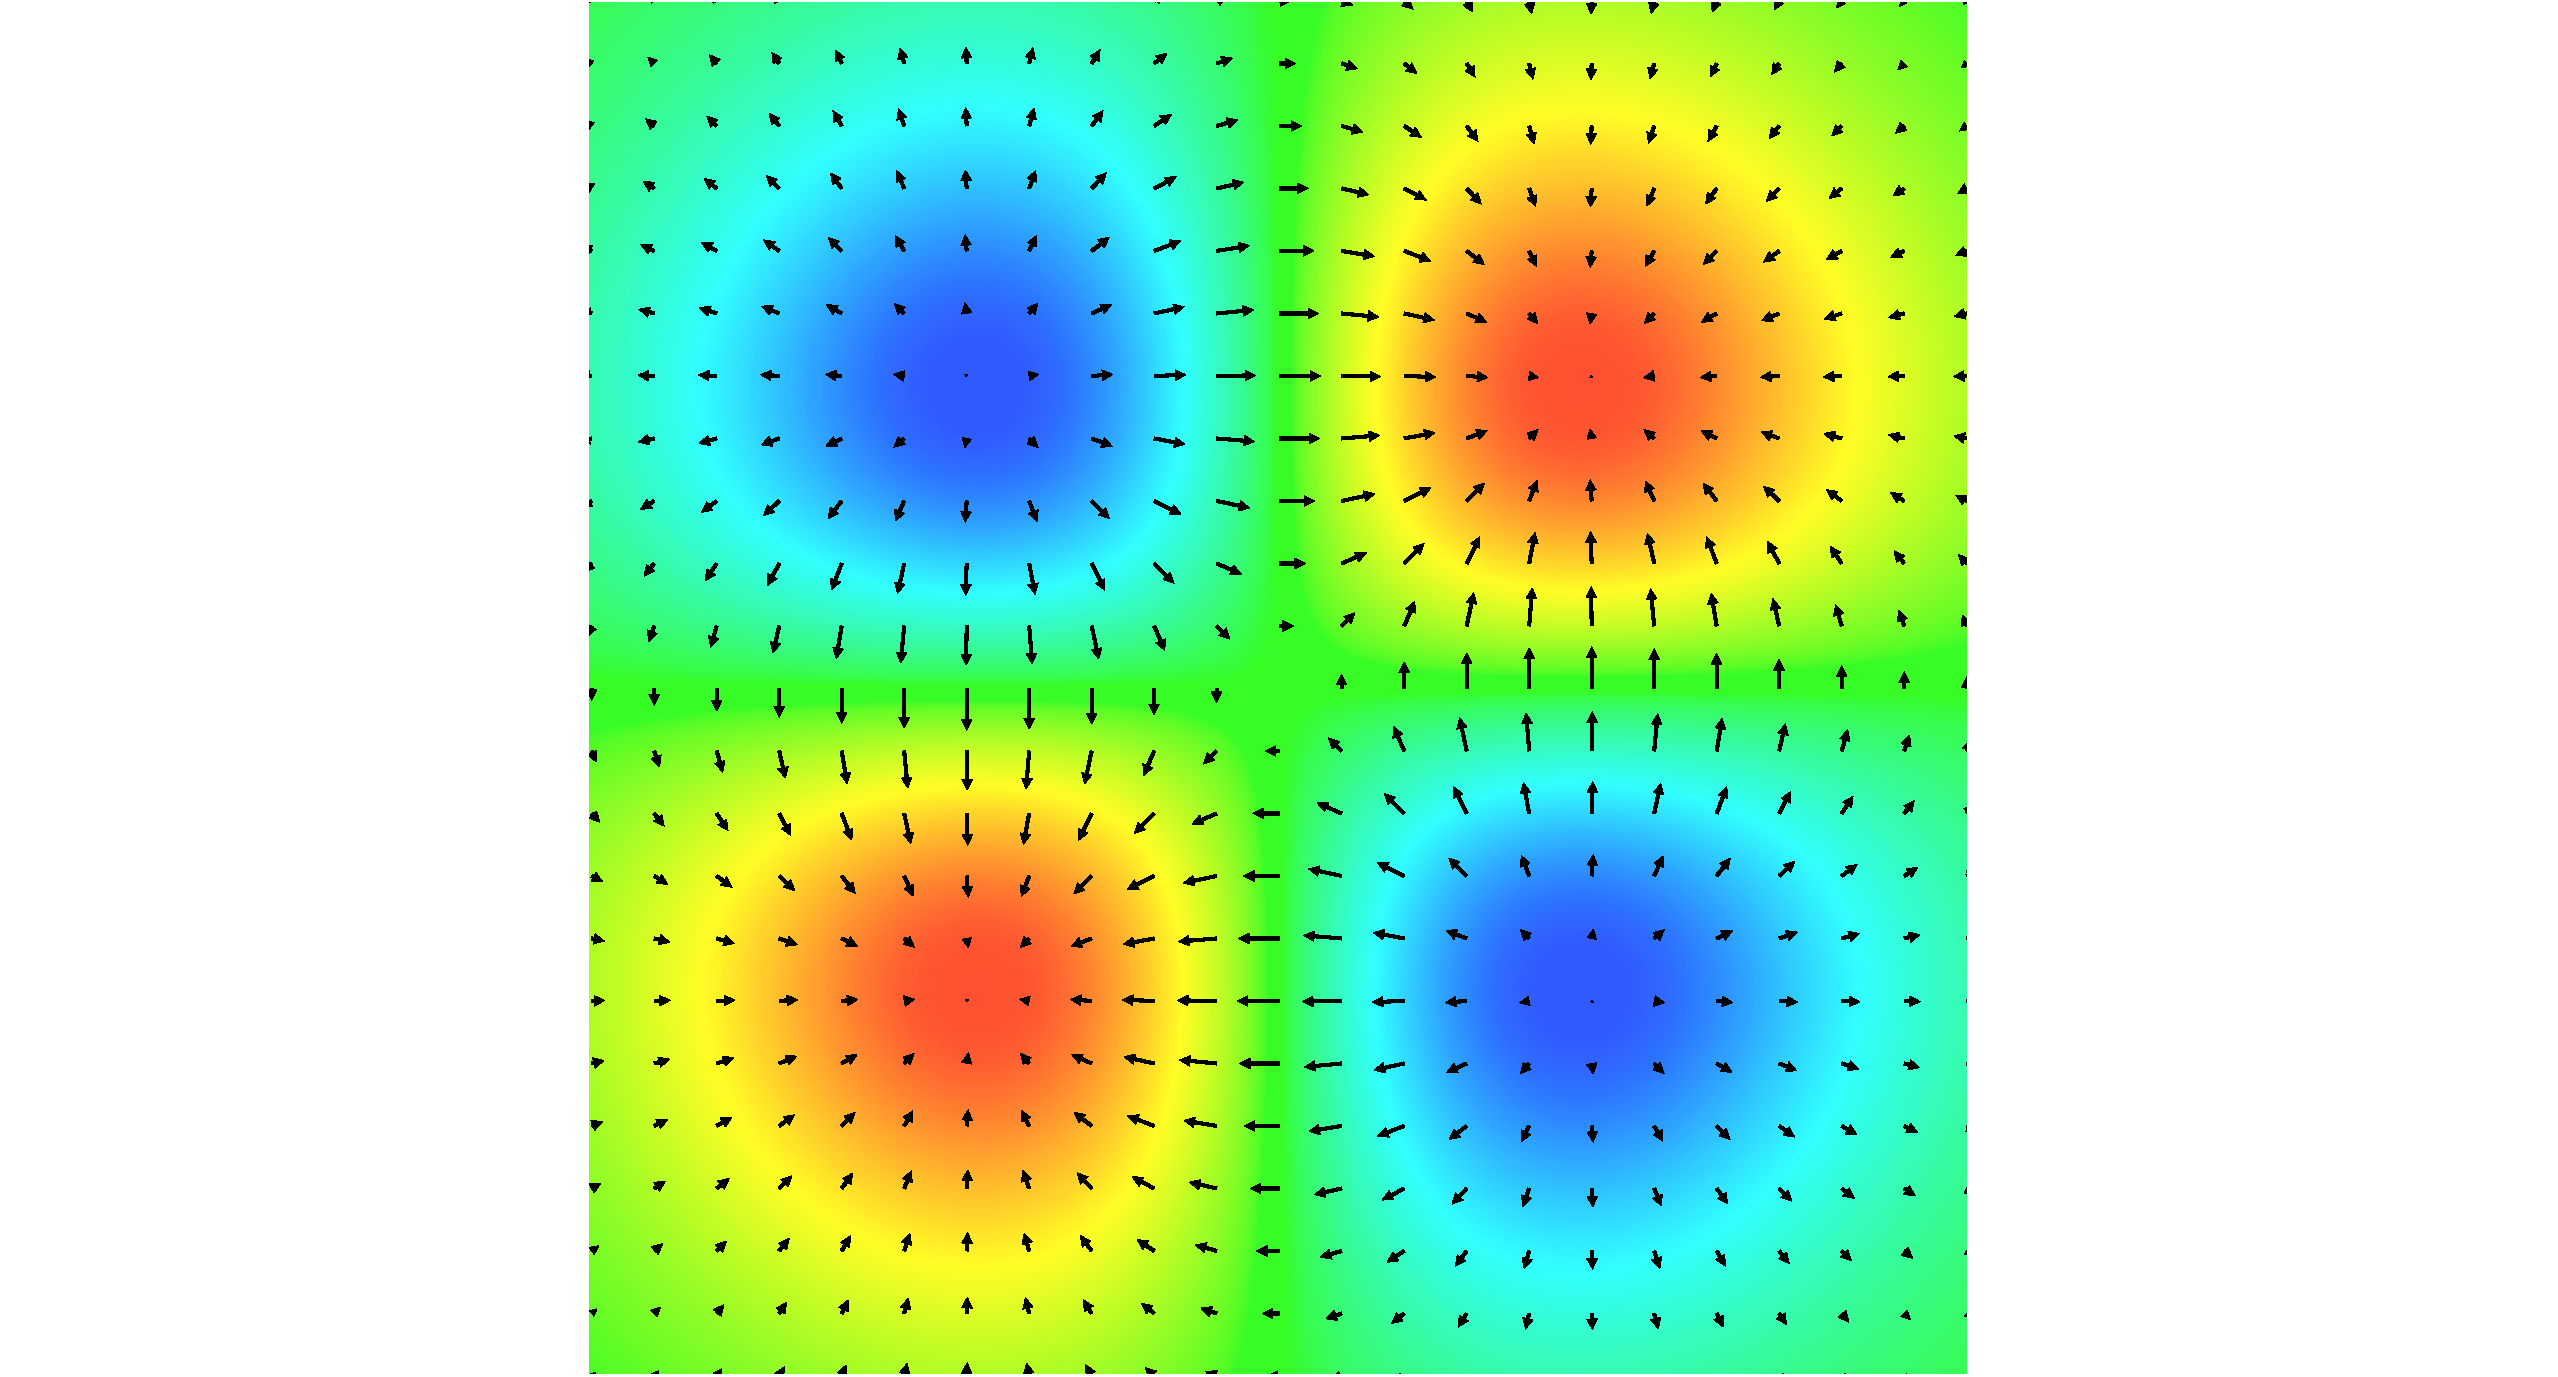
\includegraphics[width=12cm]{data/gradient2d.pdf}

  \caption{The graph of a two-dimensional scalar field, where red
    areas have large values and blue areas have small values. The
    gradient of this field is overlaid as a grid of arrows. At each
    point in the field, the gradient is in the direction of greatest
    increase, and it is larger when that rate of increase is faster.
    See figure \ref{fig:gradient3d} for a three-dimensional plot of
    this scalar field.}
  \label{fig:gradient2d}
\end{figure}

\begin{figure}[htb!] \centering

  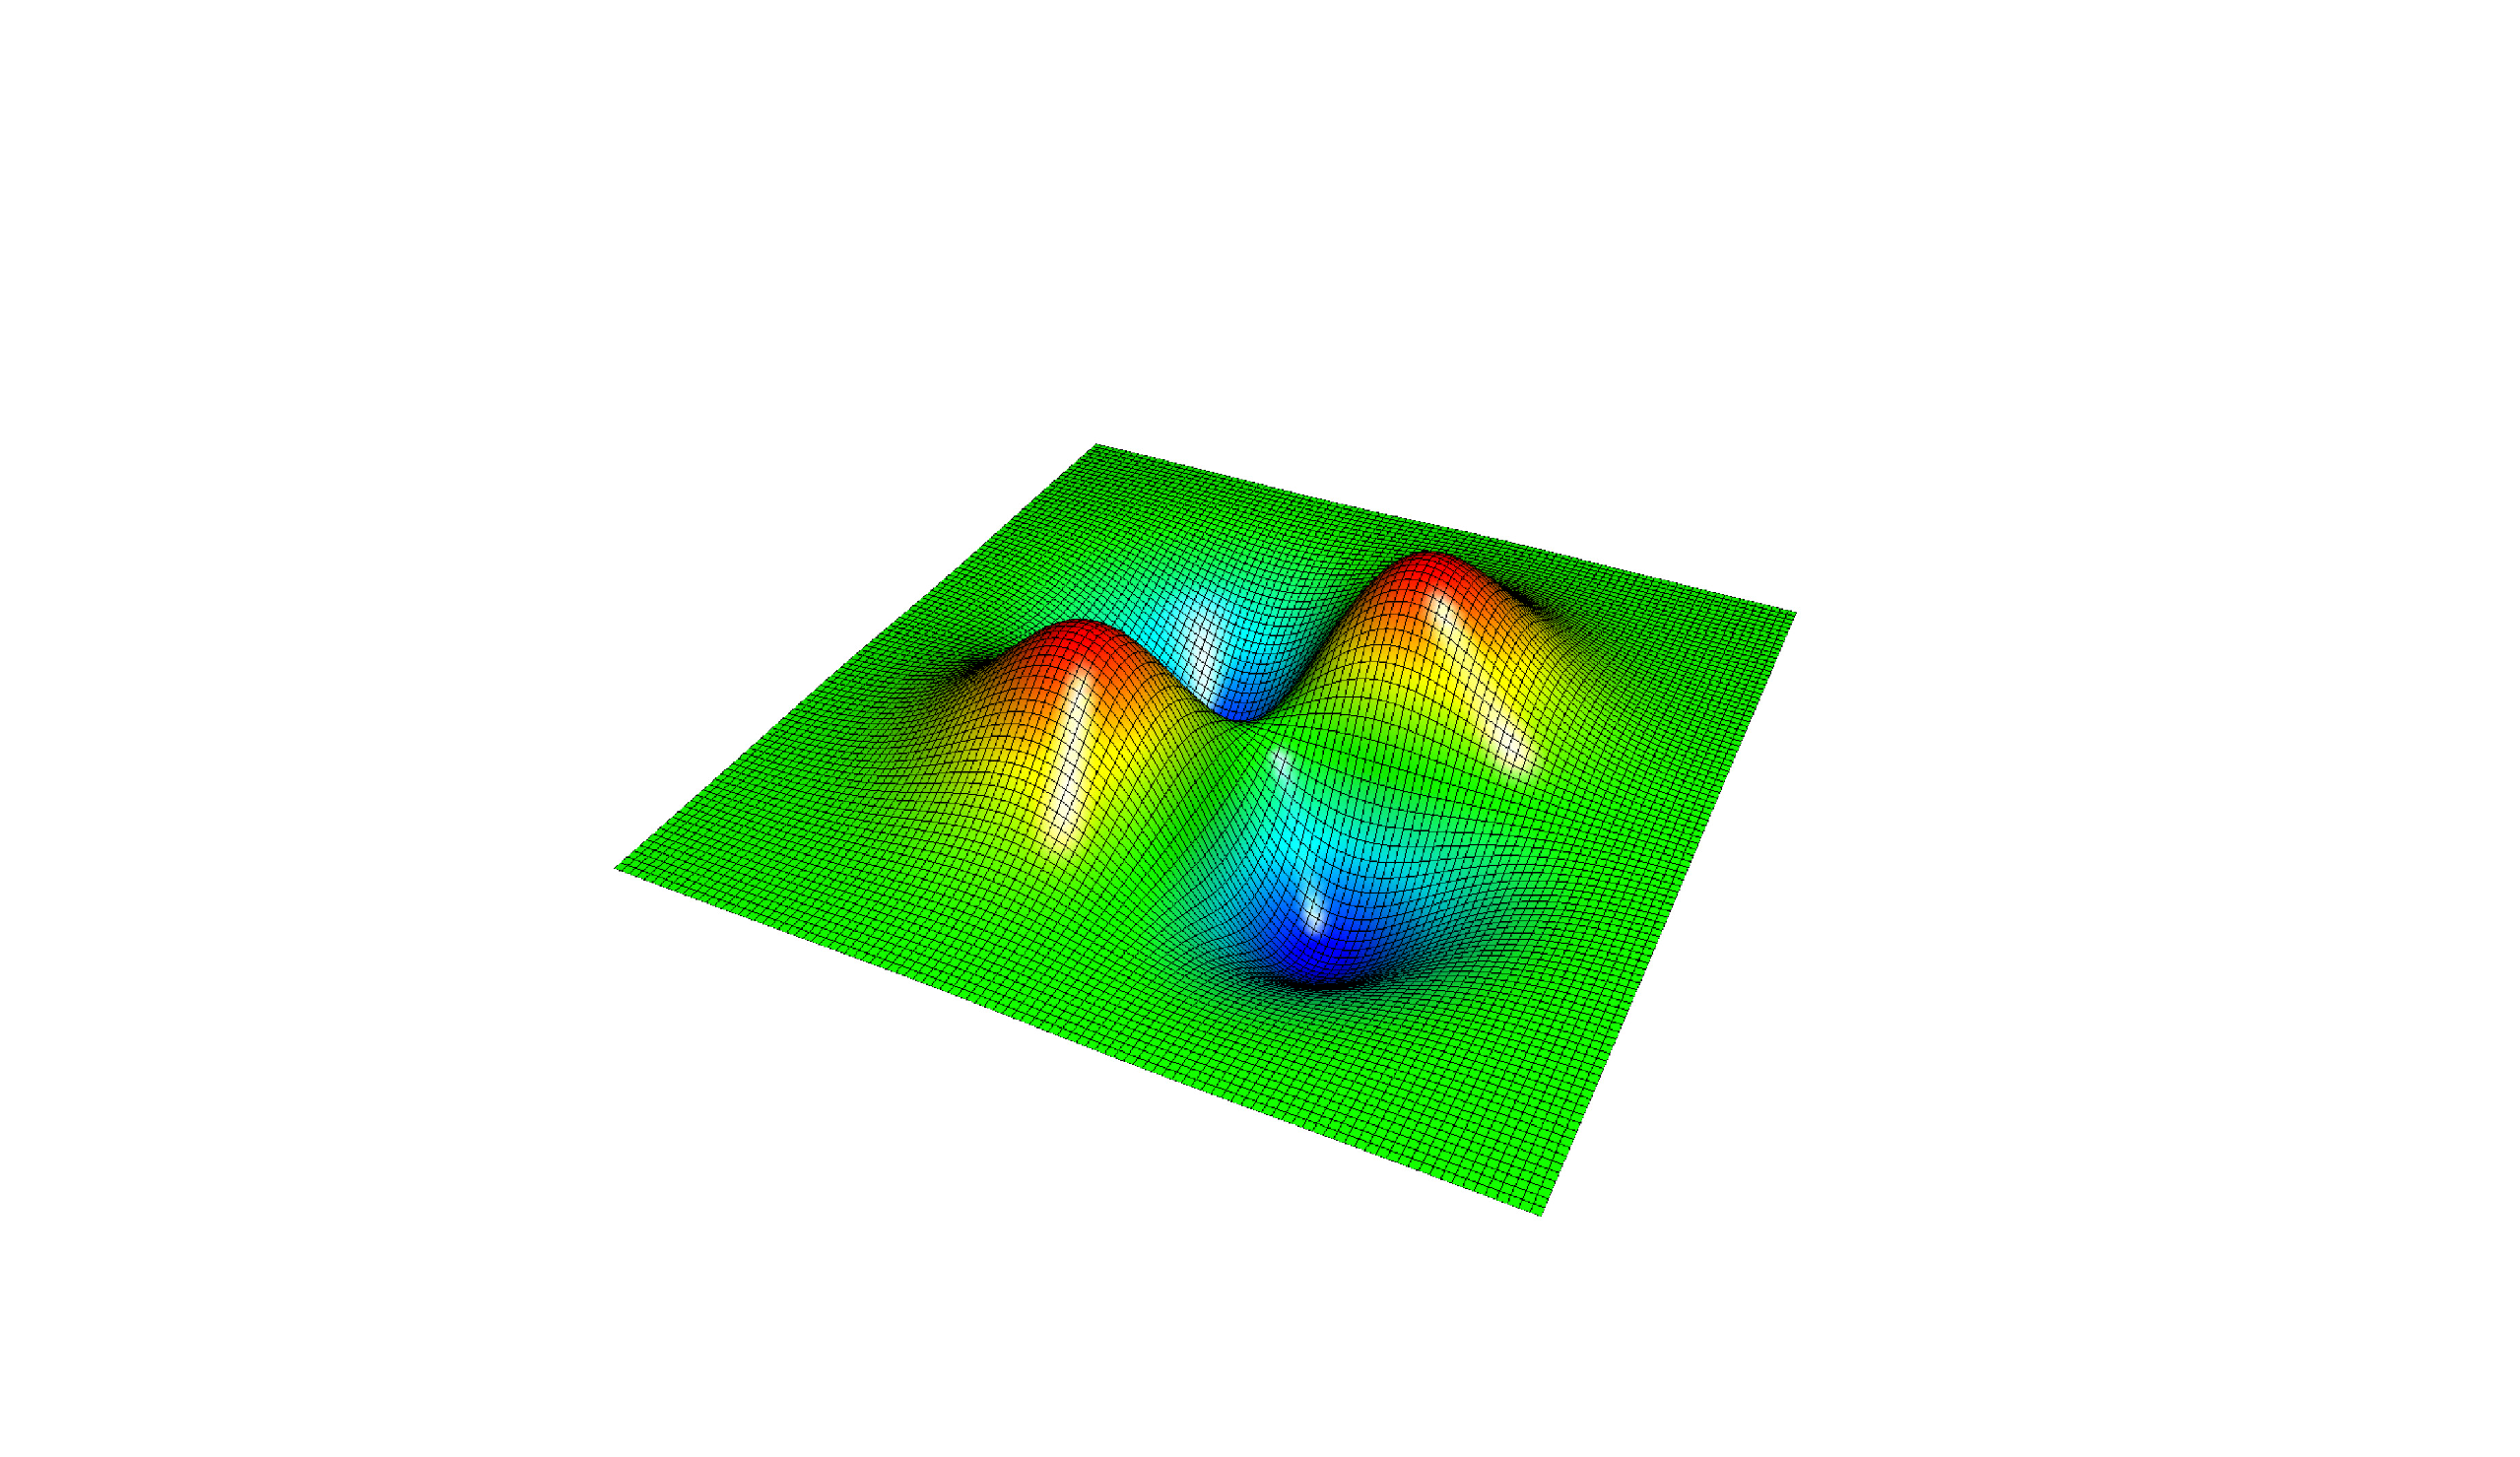
\includegraphics[width=15cm]{data/gradient3d.pdf}

  \caption{The scalar field displayed in figure \ref{fig:gradient2d}
    graphed as a function of two variables. The same colors,
    representing values of the function, are used here; and grid lines
    have been added to make the shape of the surface more evident.
    Note that the arrows in figure \ref{fig:gradient2d} are largest at
    the steepest points on this graph, and always point directly up
    the slope.}
  \label{fig:gradient3d}
\end{figure}

The gradient at a particular point is a vector pointing in the
direction of greatest increase and with a magnitude equal to that rate
of greatest increase. It should make sense that this idea is still
perfectly valid in three dimensions even though figure
\ref{fig:gradient2d} only shows a gradient in two dimensions.

\subsubsection{Definition}
\label{sec:gradient definition}

It turns out that the gradient and directional derivatives of a
function are intimately related. In fact, given just the gradient at a
single point, you can work out all of the directional derivatives at
that point! How, you ask?

Let's work with a function of two variables. To make things simpler,
instead of looking directly at the three-dimensional graph of this
function $z = f(x, y)$, let's just work with its tangent plane (which
will exist if and only if the function is differentiable). Just as the
derivative of a function is the same as the slope of its tangent line,
the directional derivative of a function is the same as the slope of
its tangent line \textit{in the same direction}. This tangent line
will, of course, be contained within the tangent plane. In figure
\ref{fig:unique plane}, the blue plane is the tangent plane to a
function at the indicated point. Figure \ref{fig:unique plane} also
shows several tangent lines to the same function, and the slope of
each one is equal to the directional derivative in the direction of
the tangent line.

In particular, the slope of the vector marked ``direction of greatest
increase'' is equal to the greatest possible directional derivative,
the slope of the vector marked ``direction of greatest decrease'' is
equal to the least possible directional derivative, the slope of the
vector marked ``direction of zero increase'' is (of course) zero, and
the slope of the vector marked ``arbitrary direction'' is somewhere in
between.

\begin{figure}[htb!] \centering

  \tdplotsetmaincoords
  {70} % increase to rotate the front of the figure upwards
  {50} % increase to rotate the front of the figure to the left

  % x-axis is toward the viewer, to the right
  % y-axis is to the right
  % z-axis is up

  \begin{tikzpicture}[tdplot_main_coords,
    every pin edge/.style={black!65, -}]

    \newcommand\pdepth{7} % width of planes
    \newcommand\vdepth{2.5} % placement of point
    \newcommand\vlength{3} % length of vectors
    \newcommand\pleft{4} % length of planes to left of point
    \newcommand\pright{4} % length of planes to right of point
    \newcommand\alength{1} % radius of angle theta
    \newcommand\rlength{0.25} % side length of right angle symbol
    \newcommand\ta{30}
    \newcommand\ra{45}

    % lower half of tilted plane
    \fill [blue, opacity=0.5] (0, 0, 0) -- (\pdepth, 0, 0)
    -- (\pdepth, {-\pleft*cos(\ta)}, {-\pleft*sin(\ta)})
    -- (0, {-\pleft*cos(\ta)}, {-\pleft*sin(\ta)}) -- cycle;
    % direction of greatest decrease
    \draw [->] (\vdepth, 0, 0)
    -- ++(0, {-\vlength*cos(\ta)}, {-\vlength*sin(\ta)})
    node[midway, pin={
      [pin distance=60]120:direction of greatest decrease}] {};
    % direction of zero increase pin
    \path (\vdepth, 0, 0) -- ++(\vlength, 0, 0)
    node[midway, pin={
      [pin distance=75]-80:direction of zero increase}] {};
    % horizontal plane
    \fill [green, opacity=0.5] (0, {-\pleft}, 0)
    -- (\pdepth, {-\pleft}, 0) -- (\pdepth, \pright, 0)
    -- (0, \pright, 0) -- cycle;
    % drop lines for direction of greatest increase
    \draw [dashed] (\vdepth, 0, 0)
    -- ++(0, {\vlength*cos(\ta)}, 0)
    -- ++(0, 0, {\vlength*sin(\ta)});
    % drop lines for arbitrary direction
    \draw [dashed] (\vdepth, 0, 0)
    -- ++({
      \vlength*cos(\ta)*sin(\ra)}, {
      \vlength*cos(\ta)*cos(\ra)}, 0)
    -- ++(0, 0, {\vlength*sin(\ta)});
    % right angle for direction of greatest increase
    \draw (\vdepth, {\vlength*cos(\ta)-\rlength}, 0)
    -- ++(0, 0, \rlength) -- ++(0, \rlength, 0);
    % right angle for arbitrary direction
    \draw ({
      \vdepth+(\vlength*cos(\ta)-\rlength)*sin(\ra)}, {
      (\vlength*cos(\ta)-\rlength)*cos(\ra)}, 0)
    -- ++(0, 0, \rlength)
    -- ++({\rlength*sin(\ra)}, {\rlength*cos(\ra)}, 0);
    % angle theta
    \draw (\vdepth, \alength, 0) arc (90:{90-\ra}:\alength)
    node[midway, above right=-5pt and 0pt, font=\footnotesize]
    {$\theta$};
    % upper half of tilted plane
    \fill [blue, opacity=0.5] (0, 0, 0) -- (\pdepth, 0, 0)
    -- (\pdepth, {\pright*cos(\ta)}, {\pright*sin(\ta)})
    -- (0, {\pright*cos(\ta)}, {\pright*sin(\ta)}) -- cycle;
    % point
    \fill (\vdepth, 0, 0) circle (2pt);
    % direction of greatest increase
    \draw [->] (\vdepth, 0, 0)
    -- ++(0, {\vlength*cos(\ta)}, {\vlength*sin(\ta)})
    node[midway, pin={
      [pin distance=60]120:direction of greatest increase}] {};
    % arbitrary direction
    \draw [->] (\vdepth, 0, 0)
    -- ++({
      \vlength*cos(\ta)*sin(\ra)}, {
      \vlength*cos(\ta)*cos(\ra)}, {
      \vlength*sin(\ta)})
    node[pos=0.85, pin={[pin distance=80]85:arbitrary direction}] {};
    % direction of zero increase
    \draw [->] (\vdepth, 0, 0) -- ++(\vlength, 0, 0);

  \end{tikzpicture}
  \caption{Various vectors pointing away from a specific point on a
    tangent plane (the blue plane), with a horizontal plane (the green
    plane) provided for reference. The slope of any given vector
    corresponds to the directional derivative in the direction of the
    vector. In particular, the vector marked ``direction of greatest
    increase'' corresponds to the maximum possible directional
    derivative, and as such is equal to the gradient of the function.}
  \label{fig:unique plane}
\end{figure}

There is one more interesting fact that you should be able to convince
yourself of if you look at figure \ref{fig:unique plane} long enough.
This is that the point marked on the figure and the direction of
greatest increase uniquely define the blue plane. In other words, it
is not possible to draw any other plane that goes through the marked
point and has the same direction of greatest increase as the blue
plane. What this means is that given just the direction and magnitude
of greatest increase (in other words, the gradient), we know the
tangent plane and therefore also every directional derivative. But how
can we find an explicit formula for any given directional derivative
in terms of the gradient?

\begin{figure}[htb!] \centering

  \tdplotsetmaincoords
  {60} % increase to look from below
  {50} % increase to look from the right

  % x-axis is toward the viewer, to the right
  % y-axis is to the right
  % z-axis is up

  \begin{tikzpicture}[tdplot_main_coords, scale=5]

    \newcommand\pleft{0.25}
    \newcommand\pright{1.25}
    \newcommand\pback{0.25}
    \newcommand\pfront{1.25}
    \newcommand\atlength{0.3}
    \newcommand\aplength{0.2}
    \newcommand\rlength{0.075}
    \newcommand\ta{30}
    \newcommand\ra{45}

    % planes [bottom tilted, horizontal]

    \fill [blue, opacity=0.2] ({-\pback}, 0, 0) -- (\pfront, 0, 0)
    -- (\pfront, {-\pleft*cos(\ta)}, {-\pleft*sin(\ta)})
    -- ({-\pback}, {-\pleft*cos(\ta)}, {-\pleft*sin(\ta)}) -- cycle;

    \fill [green, opacity=0.2] ({-\pback}, {-\pleft}, 0)
    -- (\pfront, {-\pleft}, 0) -- (\pfront, \pright, 0)
    -- ({-\pback}, \pright, 0) -- cycle;

    % dashed lines [left triangle, diagonal, right triangle]

    \draw [dashed] (0, 0, 0) -- ++(0, 1, 0) node [right] {$A$}
    -- +(0, 0, {tan(\ta)}) node [right] {$B$};

    \draw [dashed] (0, 0, 0) -- +({sin(\ra)}, {cos(\ra)}, 0);
    \draw [dashed] ({sin(\ra)}, 0, 0)
    -- ++(0, {cos(\ra)}, 0) node [right] {$C$}
    -- +(0, 0, {cos(\ra)*tan(\ta)}) node [right] {$D$};

    % planes [top tilted]
    \fill [blue, opacity=0.2] ({-\pback}, 0, 0) -- (\pfront, 0, 0)
    -- (\pfront, {\pright*cos(\ta)}, {\pright*sin(\ta)})
    -- ({-\pback}, {\pright*cos(\ta)}, {\pright*sin(\ta)}) -- cycle;

    % non-dashed lines [left hypotenuse, diagonal hypotenuse,
    % horizontal, right hypotenuse]
    \node [left] (0, 0, 0) {$O$};
    \draw (0, 0, 0) -- +(0, 1, {tan(\ta)});
    \draw (0, 0, 0) -- +({sin(\ra)}, {cos(\ra)}, {cos(\ra)*tan(\ta)});
    \draw (0, 0, 0) -- +({sin(\ra)}, 0, 0) node[below left] {$P$};
    \draw ({sin(\ra)}, 0, 0) -- +(0, {cos(\ra)}, {cos(\ra)*tan(\ta)});

    % angles theta and phi

    \draw (0, \atlength, 0) arc (90:{90-\ra}:\atlength)
    node [midway, above right=-7pt and 1pt] {$\theta$};

    \draw (\aplength, 0, 0) arc (0:\ra:\aplength)
    node [midway, below right=-6pt and 1pt] {$\phi$};

    % right angles [left triangle, diagonal triangle, right triangle,
    % horizontal triangle]

    \draw [black!65] (0, {1-\rlength}, 0)
    -- ++(0, 0, \rlength) -- +(0, \rlength, 0);

    \draw [black!65] ({
      (1-\rlength)*sin(\ra)}, {
      (1-\rlength)*cos(\ra)}, 0)
    -- ++(0, 0, \rlength)
    -- +({\rlength*sin(\ra)}, {\rlength*cos(\ra)}, 0);

    \draw [black!65] ({sin(\ra)}, {cos(\ra)-\rlength}, 0)
    -- ++(0, 0, \rlength) -- +(0, \rlength, 0);

    \draw [black!65] ({sin(\ra)-\rlength}, 0, 0)
    -- ++(0, \rlength, 0) -- +(\rlength, 0, 0);

  \end{tikzpicture}
  \caption{Two directional derivatives differing by an angle $\theta$,
    where one is in the direction of maximum increase, are visualized
    here as line segments with slopes equal to the corresponding
    derivatives. A second right triangle parallel to
    $\bigtriangleup OAB$ has been added to the other elements present
    in figure \ref{fig:unique plane}.}
  \label{fig:gradient geometry}
\end{figure}

It's time for some good old-fashioned coordinate geometry. Using
figure \ref{fig:gradient geometry}, we can associate several of the
quantities we are discussing with geometric properties. On the figure
we have drawn two right triangles: one in the direction of maximum
increase ($\bigtriangleup OAB$) and one in an arbitrary other
direction that differs from the first by an angle $\theta$
($\bigtriangleup OCD$). If we draw these triangles such that their
bases ($OA$ and $OC$) both have lengths of $1$, then the slopes of the
hypotenuses will be the lengths of $AB$ and $CD$ respectively. First,
we can use the angle $\phi$ to do some trigonometry on
$\bigtriangleup OPC$. In particular, we have $\sin \phi = PC/OC = PC$
because $OC$ is of length $1$. Since the angles $\phi$ and $\theta$
are complementary, we have $\sin \phi = \cos \theta$ and so
$PC = \cos \theta$. Now note that $OB$ and $PD$ are parallel, and so
their angles $\angle AOB$ and $\angle CPD$ are congruent: both are
equal to the angle of elevation of the blue plane relative to the
horizontal green plane. Since $\bigtriangleup OAB$ and
$\bigtriangleup PCD$ are right triangles with one congruent angle, all
of their angles are congruent and so the triangles are similar. This
means that we can equate the ratios $OA/AB = PC/CD$, or in other words
$1/AB = \cos \theta/CD$, where we have used the facts from earlier
that $OA = 1$ and $PC = \cos \theta$. We can rewrite this equation to
see that $CD = AB \cos \theta$.

Now all that is left is to translate this geometric property back into
the language of vectors. Recall that $AB$ is the slope of $OB$, which
is the rate of maximum increase, which is the magnitude of the
gradient. Recall also that $CD$ is the slope of $OD$, which is the
rate of increase in the direction $\theta$ away from the direction of
maximum increase, which is the directional derivative in this
direction. We then have $D_{\vec u} f = |\grad f| \cos \theta$, where
$D_{\vec u} f$ is the directional derivative in the direction of
$\vec{u}$ and $\vec{u}$ is a unit vector in the direction of $OD$.
There you have it!

But there is an even more convenient form of this equation. Recall the
geometric formula for the dot product,
$\vec{a} \cdot \vec{b} = |\vec{a}| |\vec{b}| \cos \theta$. If
$\vec{b}$ is a unit vector $\vec{u}$, then we have $|\vec{u}| = 1$ and
so $\vec{a} \cdot \vec{u} = |\vec{a}| \cos \theta$. Wow -- that looks
familiar! All we have to do is let $\vec{a} = \grad f$ and we have
that $\grad f \cdot \vec{u} = |\grad f| \cos \theta = D_{\vec{u}} f$.
So we have proved that the dot product of the gradient with
\textit{any} unit vector is the directional derivative in that
direction.

Because the component of $\vec{v}$ in the direction of the unit vector
$\vec{u}$ is $\vec{v} \cdot \vec{u}$, we need only let
$\vec{v} = \grad f$ to see that the component of the gradient in any
direction is the directional derivative in that direction. Thus, we
have arrived at another, subtler, intuitive interpretation of the
gradient!

Typically, the gradient is defined as the unique vector whose
component in any given direction is the directional derivative in that
direction. I, however, think that it is more natural to start with the
definition of the gradient as the direction and magnitude of maximum
increase and derive the component definition from there.

\subsubsection{Definition with Partial Derivatives}
\label{sec:gradient definition with partial derivatives}

The gradient also has a formula in terms of partial derivatives. It is
quite easy, really: if we want to express the gradient in terms of
$\ih$, $\jh$, and $\kh$, all we need are the components of the
gradient in those three directions. We already showed that the
component of the gradient in any given direction is simply the
directional derivative in that direction. In fact, the directional
derivatives in the $\ih$, $\jh$, and $\kh$ directions already have
names: they are better known as the partial derivatives with respect
to $x$, $y$, and $z$. So the gradient is also given by:
\[
  \grad f =
  \frac{\partial f}{\partial x} \ih +
  \frac{\partial f}{\partial y} \jh +
  \frac{\partial f}{\partial z} \kh.
\]

The nice, symmetric form taken by this last form of the gradient has
inspired mathematicians to write the equation in the following form:
\[
  \grad f = \left(
    \frac{\partial}{\partial x} \ih +
    \frac{\partial}{\partial y} \jh +
    \frac{\partial}{\partial z} \kh
  \right)f.
\]
If you pretend, for a moment, that a vector made up of partial
derivative operators is even a legitimate mathematical structure (of
course, it is not, but bear with me for a moment here), and simply
multiply the ``vector'' by the ``scalar'' $f$, then you will get the
previous formula for the gradient in terms of partial derivatives. For
convenience, many people like to call the ``vector'' of partial
derivative operators by the name ``del'' or ``nabla'', written as
$\del$ (you may see this symbol as $\nabla$ but I think it should be
in \textbf{boldface} because it is a vector). These people then like
to write the gradient as
\[
  \grad f = \del f.
\]
I think it's a little confusing, but you can write it however you
like. Any good mathematician (or student) should understand either.

\subsection{The Gradient Theorem}
\label{sec:gradient theorem}

\begin{prereq}
  Understand the gradient (see section \ref{sec:gradient}), the proof
  of the first fundamental theorem of calculus (see section
  \ref{sec:ftc}), and line integrals.
\end{prereq}

\subsubsection{The Equation}
\label{sec:gradient theorem equation}

The gradient theorem is a generalization of the first fundamental
theorem of calculus to a curved path rather than a straight line.
Recall that the fundamental theorem is calculus is:
\[
  \int_a^b f'(x) \,dx = f(b) - f(a).
\]
The gradient theorem is:
\[
  \int_\vec{a}^\vec{b} \grad f(\vec{x}) \cdot d\vec{x}
  = f(\vec{b}) - f(\vec{a}).
\]
In this equation, $f$ is a function of multiple variables, but rather
than writing $f(x, y)$ we just let $\vec{x} = x \ih + y \jh$ and say
$f(\vec{x})$. You can see that although the left-hand side is a line
(or path, or contour) integral, the path is not given. In fact,
according to the gradient theorem, the integral is the same value,
$f(\vec{b}) - f(\vec{a})$, no matter what path is used!

You may also see the gradient theorem written in the following
equivalent form:
\[
  \int_\vec{a}^\vec{b} \del f \cdot d\vec{x} = f(\vec{b}) - f(\vec{a}).
\]

\subsubsection{The Proof}
\label{sec:gradient theorem proof}

In any case, the important thing is understanding why the theorem is
true. You may wish to review section \ref{sec:ftc} -- and in
particular \ref{sec:ftc alternate proof} -- because the proof of the
gradient theorem is exactly analogous to that of the first fundamental
theorem of calculus.

\renewcommand{\arraystretch}{2}
\begin{longtable}{|p{0.4\textwidth}|p{0.5\textwidth}|}

  \hline

  First fundamental theorem of calculus &
  Gradient theorem in two dimensions \\

  \hline

  The total change in $y$ is $\Delta y = f(b) - f(a)$. &
  The total change in $z$ is $\Delta z = f(\vec{b}) - f(\vec{a})$. \\

  The interval from $a$ to $b$ can be split into many subintervals,
  each of which has a $\Delta x_i$. Over each subinterval, the value
  of $f(x)$ will change by $\Delta y_i$. &

  The curve from $\vec{a}$ to $\vec{b}$ can be split into many small
  sections of curve, each of which has a $\Delta x_i$ and $\Delta
  y_i$. Over each section of curve, the value of $f(\vec{x})$ will
  change by $\Delta z_i$. \\

  We can approximate $\Delta y_i$ using the tangent line to the
  function. &

  We can approximate $\Delta z_i$ using the tangent plane to the
  function. \\

  The tangent line has a slope of $\frac{df}{dx}$, so changing $x$ by
  $\Delta x_i$ will change $y$ by $\frac{df}{dx} \Delta x_i$. &

  We can split the change in $z$ into two parts: the part due to
  changing $x$ and the part due to changing $y$. The tangent plane has
  a slope of $\frac{\partial f}{\partial x}$ in the $x$ direction, so
  changing $x$ by $\Delta x_i$ will change $z$ by $\frac{\partial
    f}{\partial x} \Delta x_i$. On the other hand, the tangent plane
  has a slope of $\frac{\partial f}{\partial y}$ in the $y$ direction,
  so changing $y$ by $\Delta y_i$ will change $z$ by $\frac{\partial
    f}{\partial y} \Delta y_i$. Since we change both $x$ and $y$, we
  can simply add the two resulting changes in $z$ together to get the
  total change in $z$. \\

  Therefore, $\Delta y_i \approx \frac{df}{dx} \Delta x_i$. &

  Therefore, $\Delta z_i \approx \frac{\partial f}{\partial x} \Delta
  x_i + \frac{\partial f}{\partial y} \Delta y_i$. \\

  Since adding together all of the $\Delta y_i$ will give us the total
  $\Delta y = f(b) - f(a)$, we have

  {\begin{align*}
     f(b) - f(a)
     &= \sum_i \Delta y_i \\
     &\approx \sum_i \frac{df}{dx} \Delta x_i \\
     &\approx \sum_i f'(x) \Delta x_i \\
     &= \int_a^b f'(x) \,dx.
   \end{align*}} &

 Since adding together all of the $\Delta z_i$ will give us the total
 $\Delta z = f(\vec{b}) - f(\vec{a})$, we have

 {\begin{align*}
    f(\vec{b})
    & - f(\vec{a}) = \sum_i \Delta z_i \\
    &\approx \sum_i \frac{\partial f}{\partial x} \Delta x_i
      + \frac{\partial f}{\partial y} \Delta y_i \\
    &\approx \sum_i \left(
      \frac{\partial f}{\partial x} \ih
      + \frac{\partial f}{\partial y} \jh
      \right) \cdot \left(
      \Delta x_i \ih + \Delta y_i \jh\right) \\
    &\approx \sum_i \left(\grad f\right)
      \cdot \left(\Delta \vec{x}_i\right) \\
    &= \int_\vec{a}^\vec{b} \grad f \cdot d\vec{x}.
  \end{align*}} \\

\hline

\end{longtable}

Although this proof was for functions of two variables, it is quite
easy to extend it to functions of three variables. In general, the
gradient theorem is true for any number of dimensions.

Also, note that we made no reference in the proof to the overall shape
of the path of the line integral; thus, the path must not affect the
value of the integral!

\subsection{The Divergence}
\label{sec:divergence}

\begin{prereq}
  Understand line integrals, surface integrals, their interpretations
  as flux, and partial derivatives.
\end{prereq}

\subsubsection{Intuition}
\label{sec:divergence intuition}

The divergence is an operation that takes a vector field $\vec{F}$ and
returns a scalar field, $\div \vec{F}$. Be careful, though, that you
do not think the divergence and gradient are inverse functions!

The most intuitive way to visualize the divergence is with a
\textit{velocity field}. Given a region (two-dimensional or
three-dimensional) filled with moving liquid, at each point the liquid
is moving a certain velocity, which is a vector (direction and
magnitude). Four velocity fields are pictured in figure
\ref{fig:velocity fields}.

\begin{figure}[htb!] \centering
  \begin{tabular}{cc}
    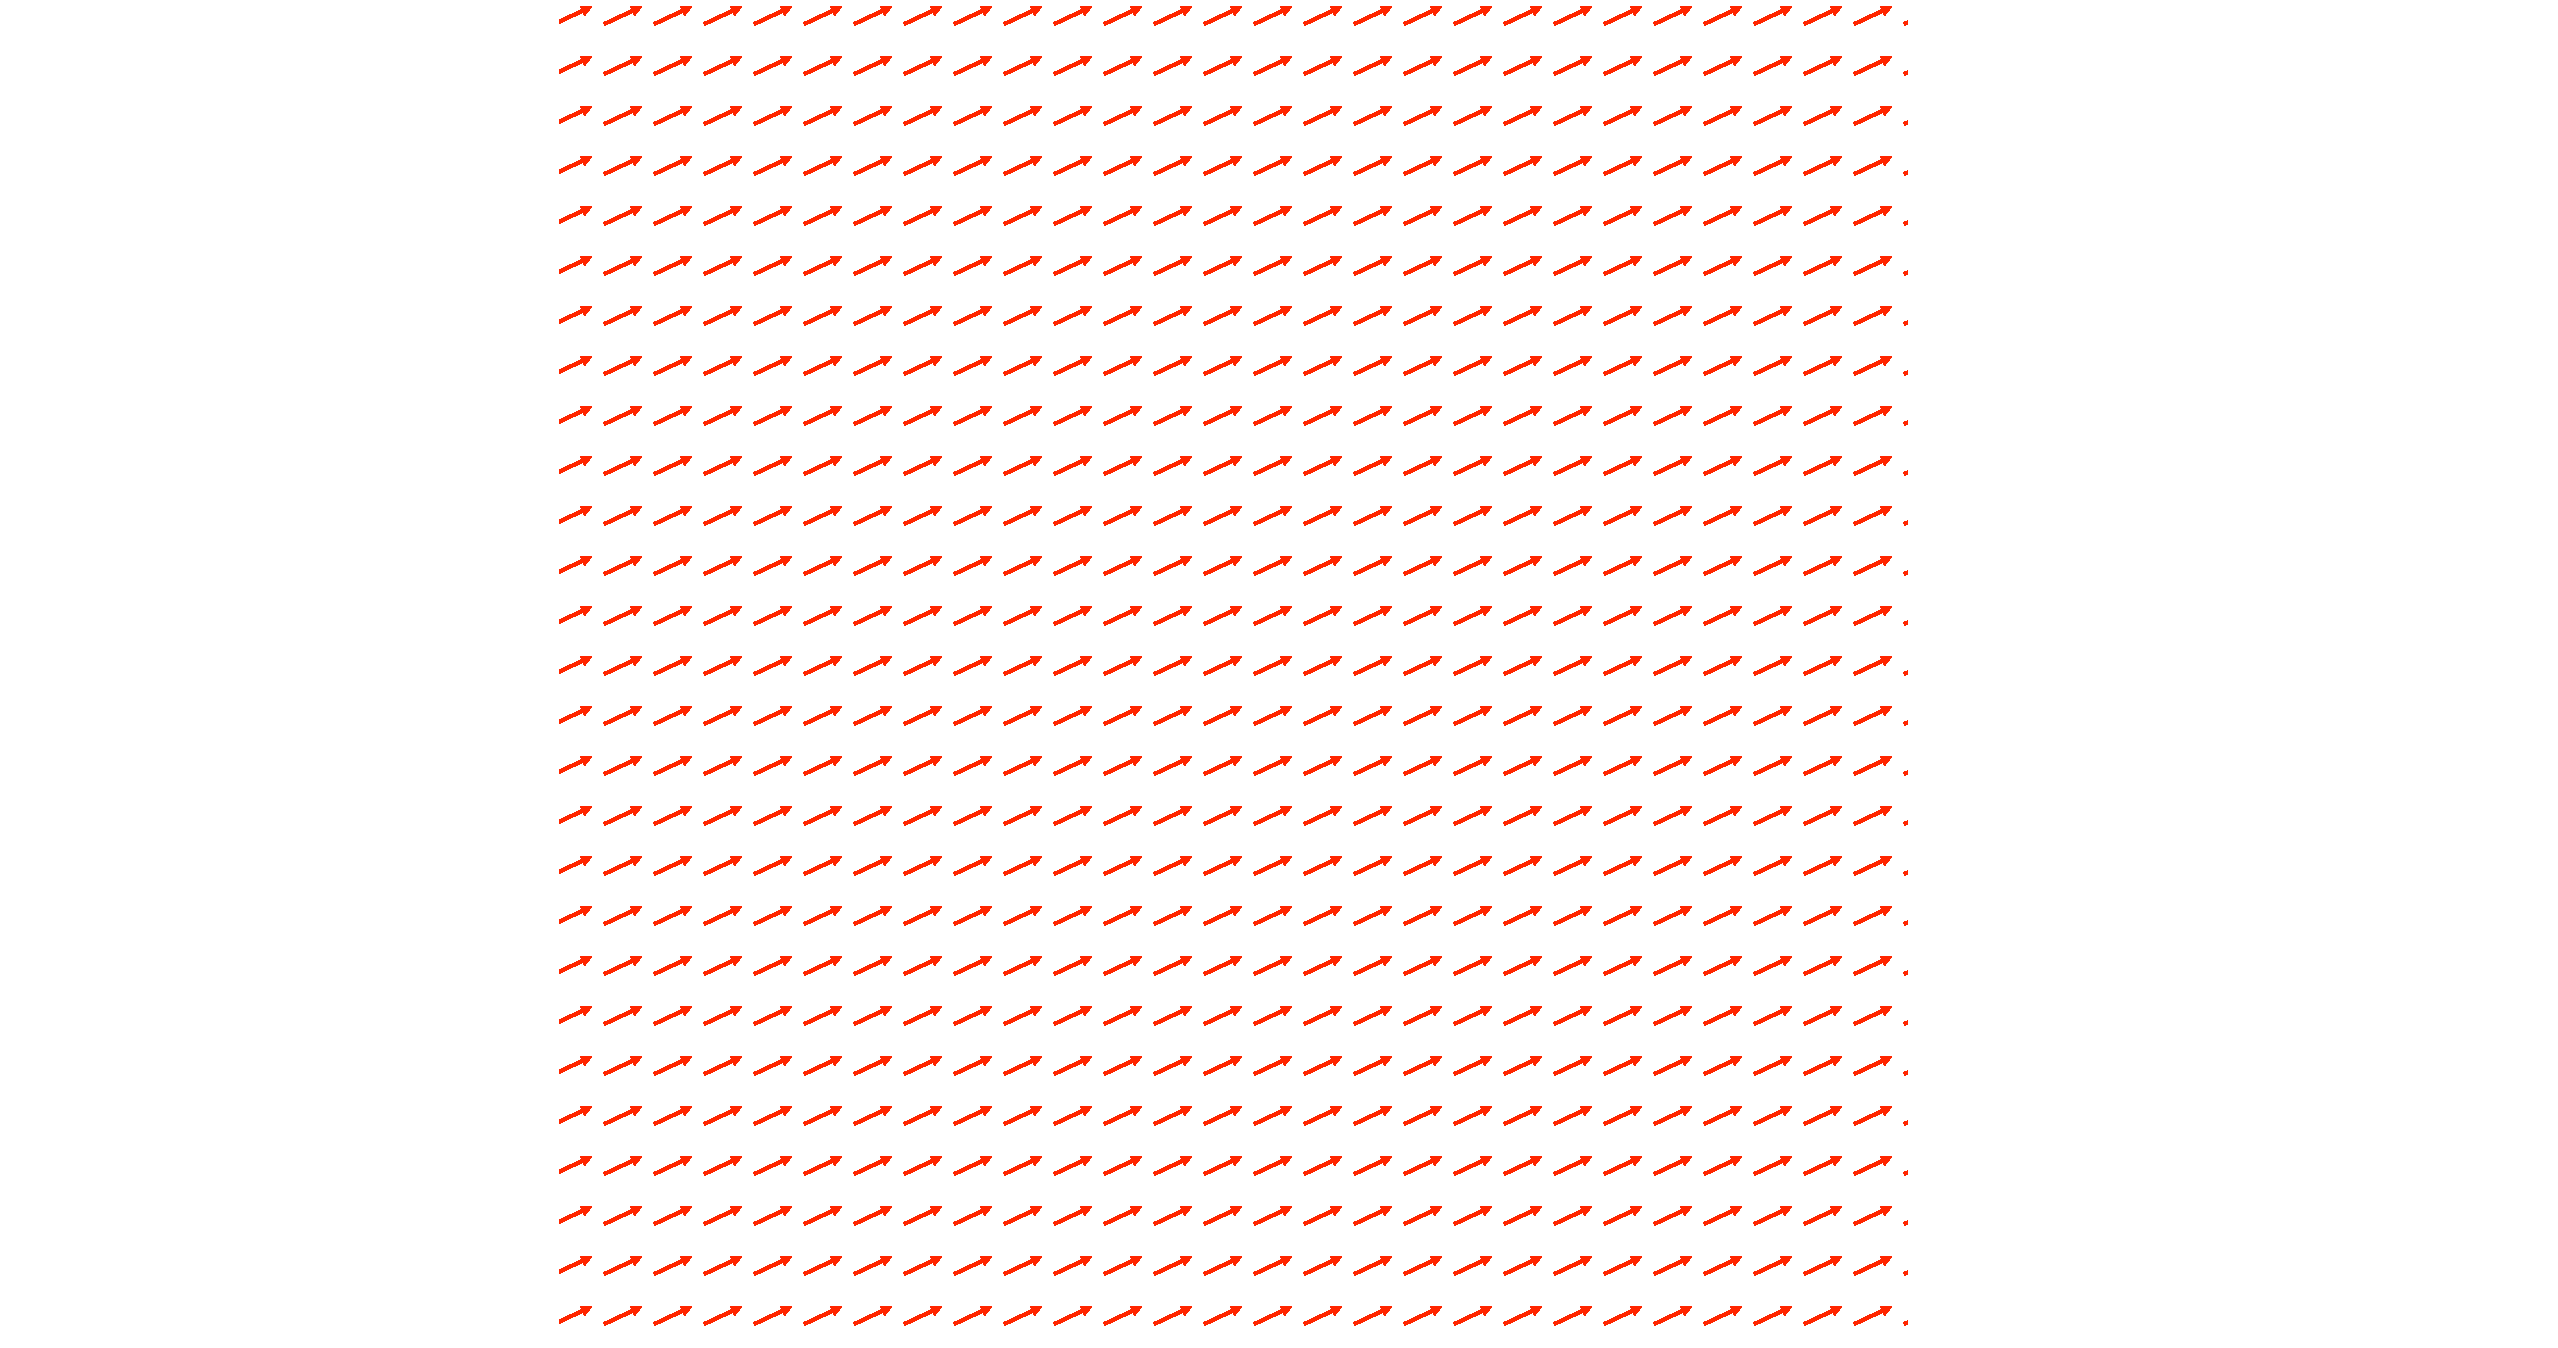
\includegraphics[width=65mm]{data/velocityfield1.pdf}
    & 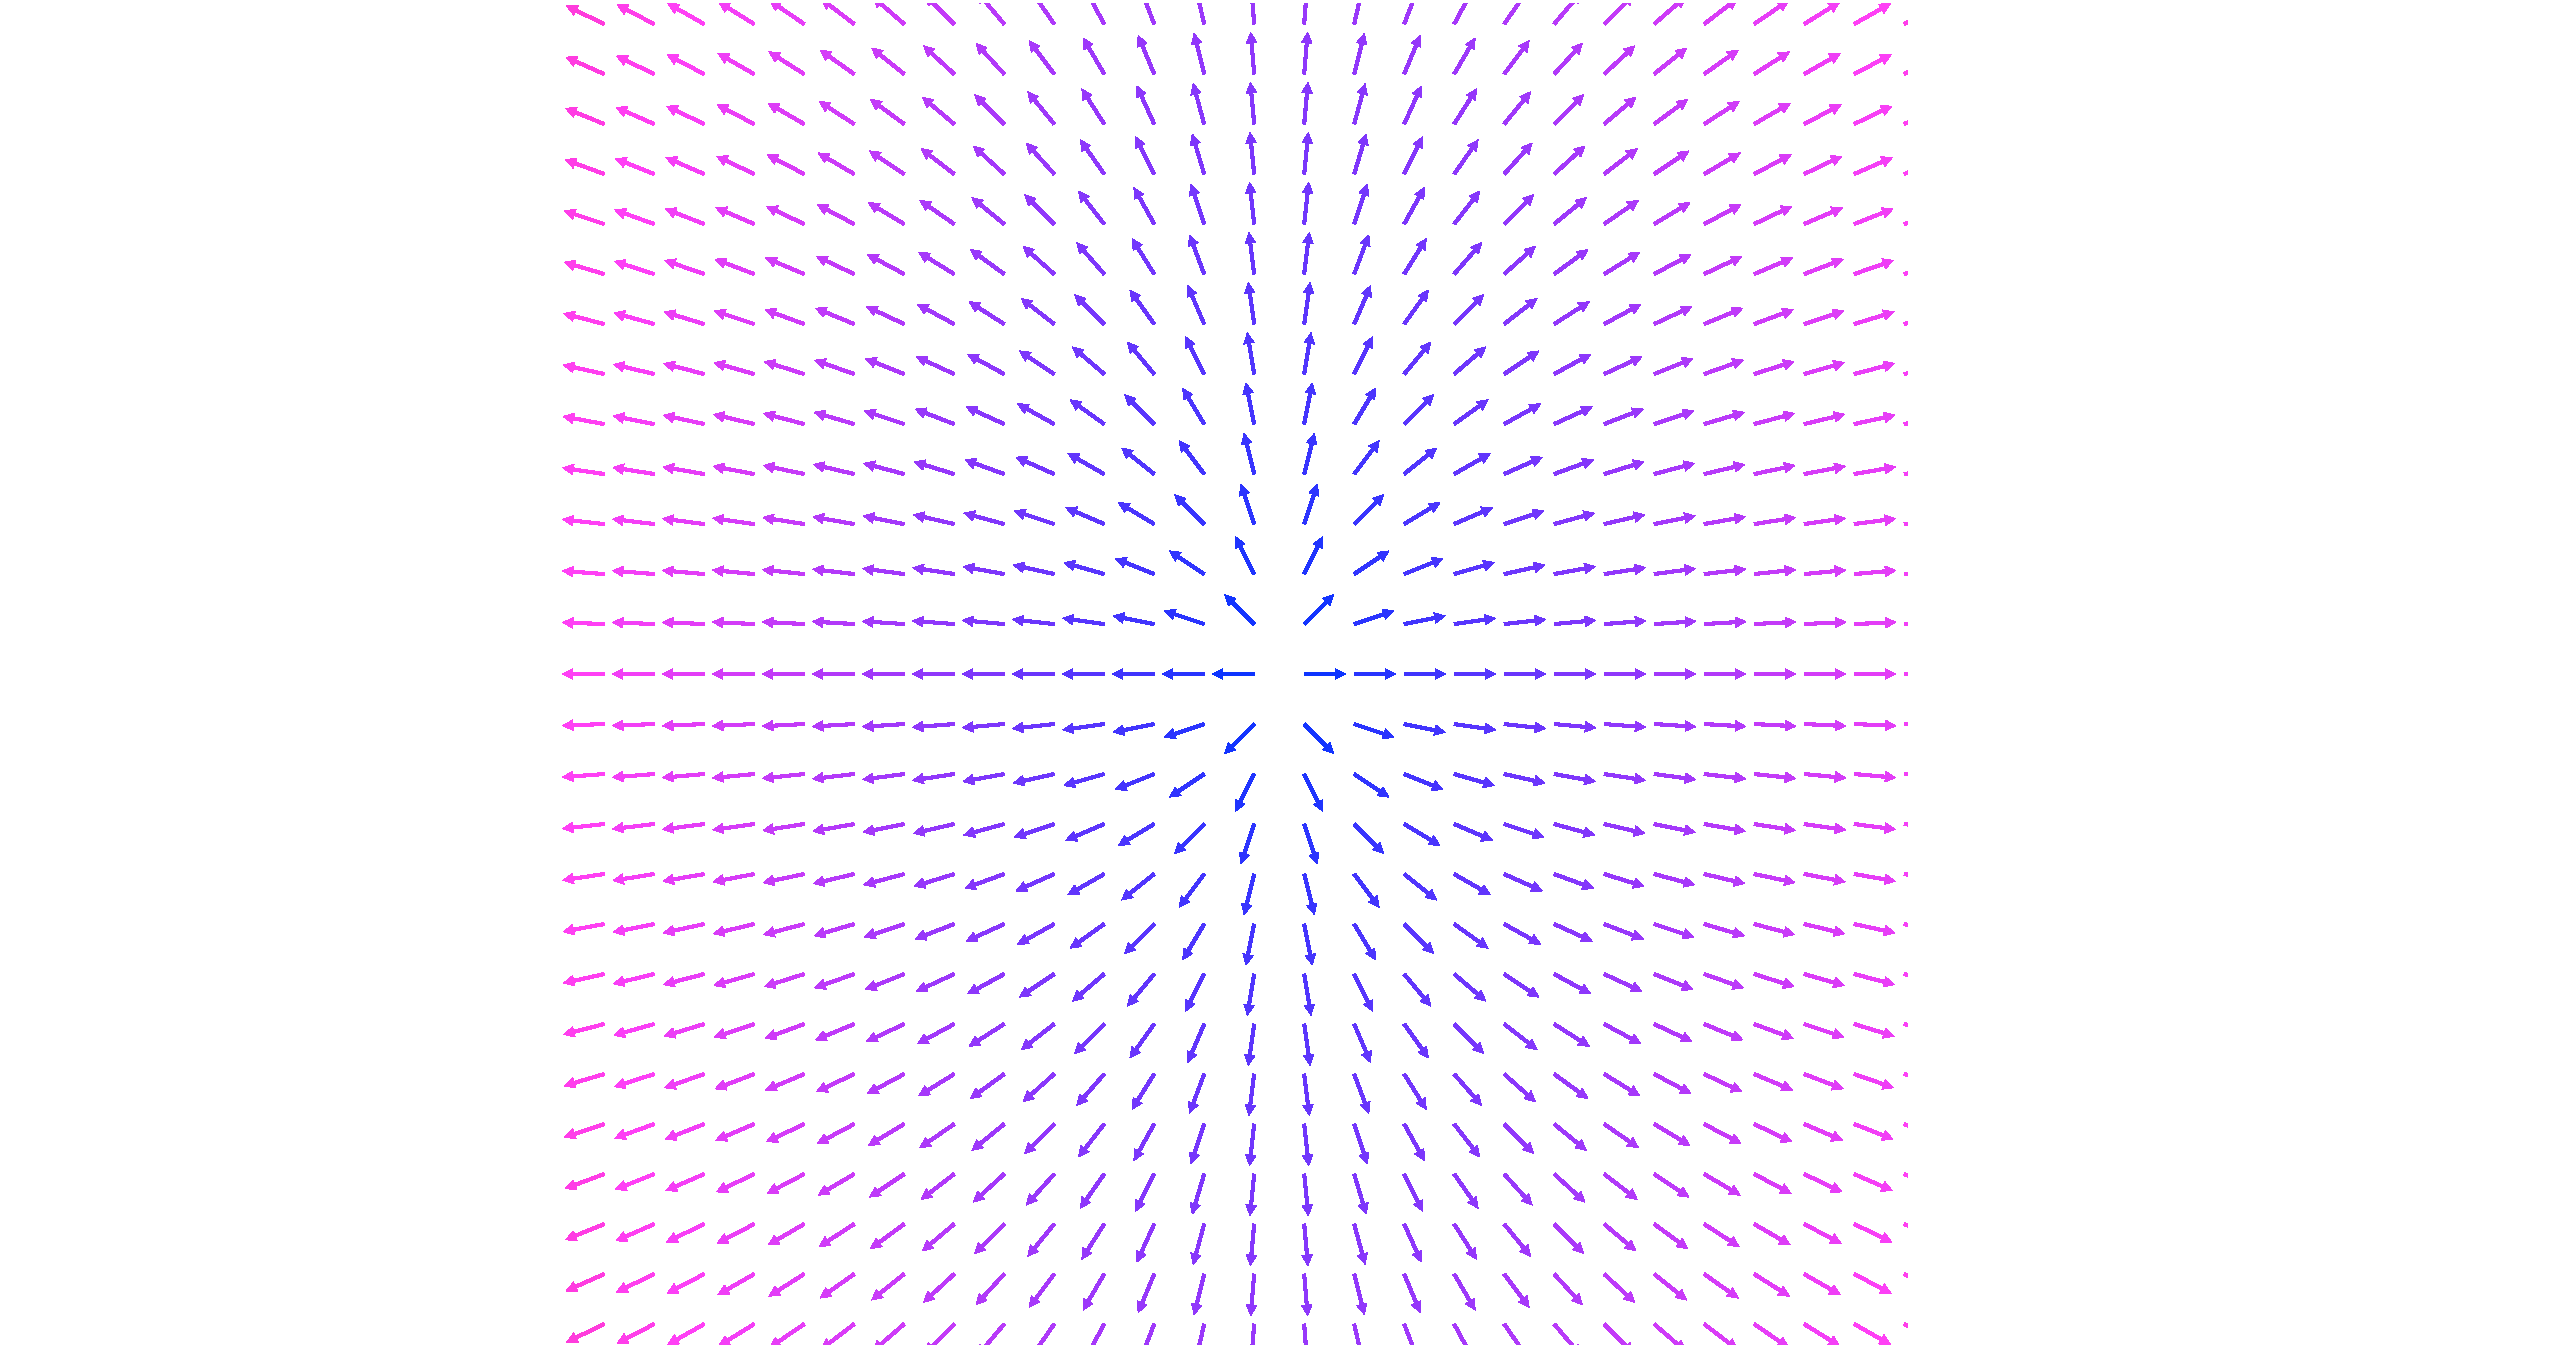
\includegraphics[width=65mm]{data/velocityfield2.pdf} \\
    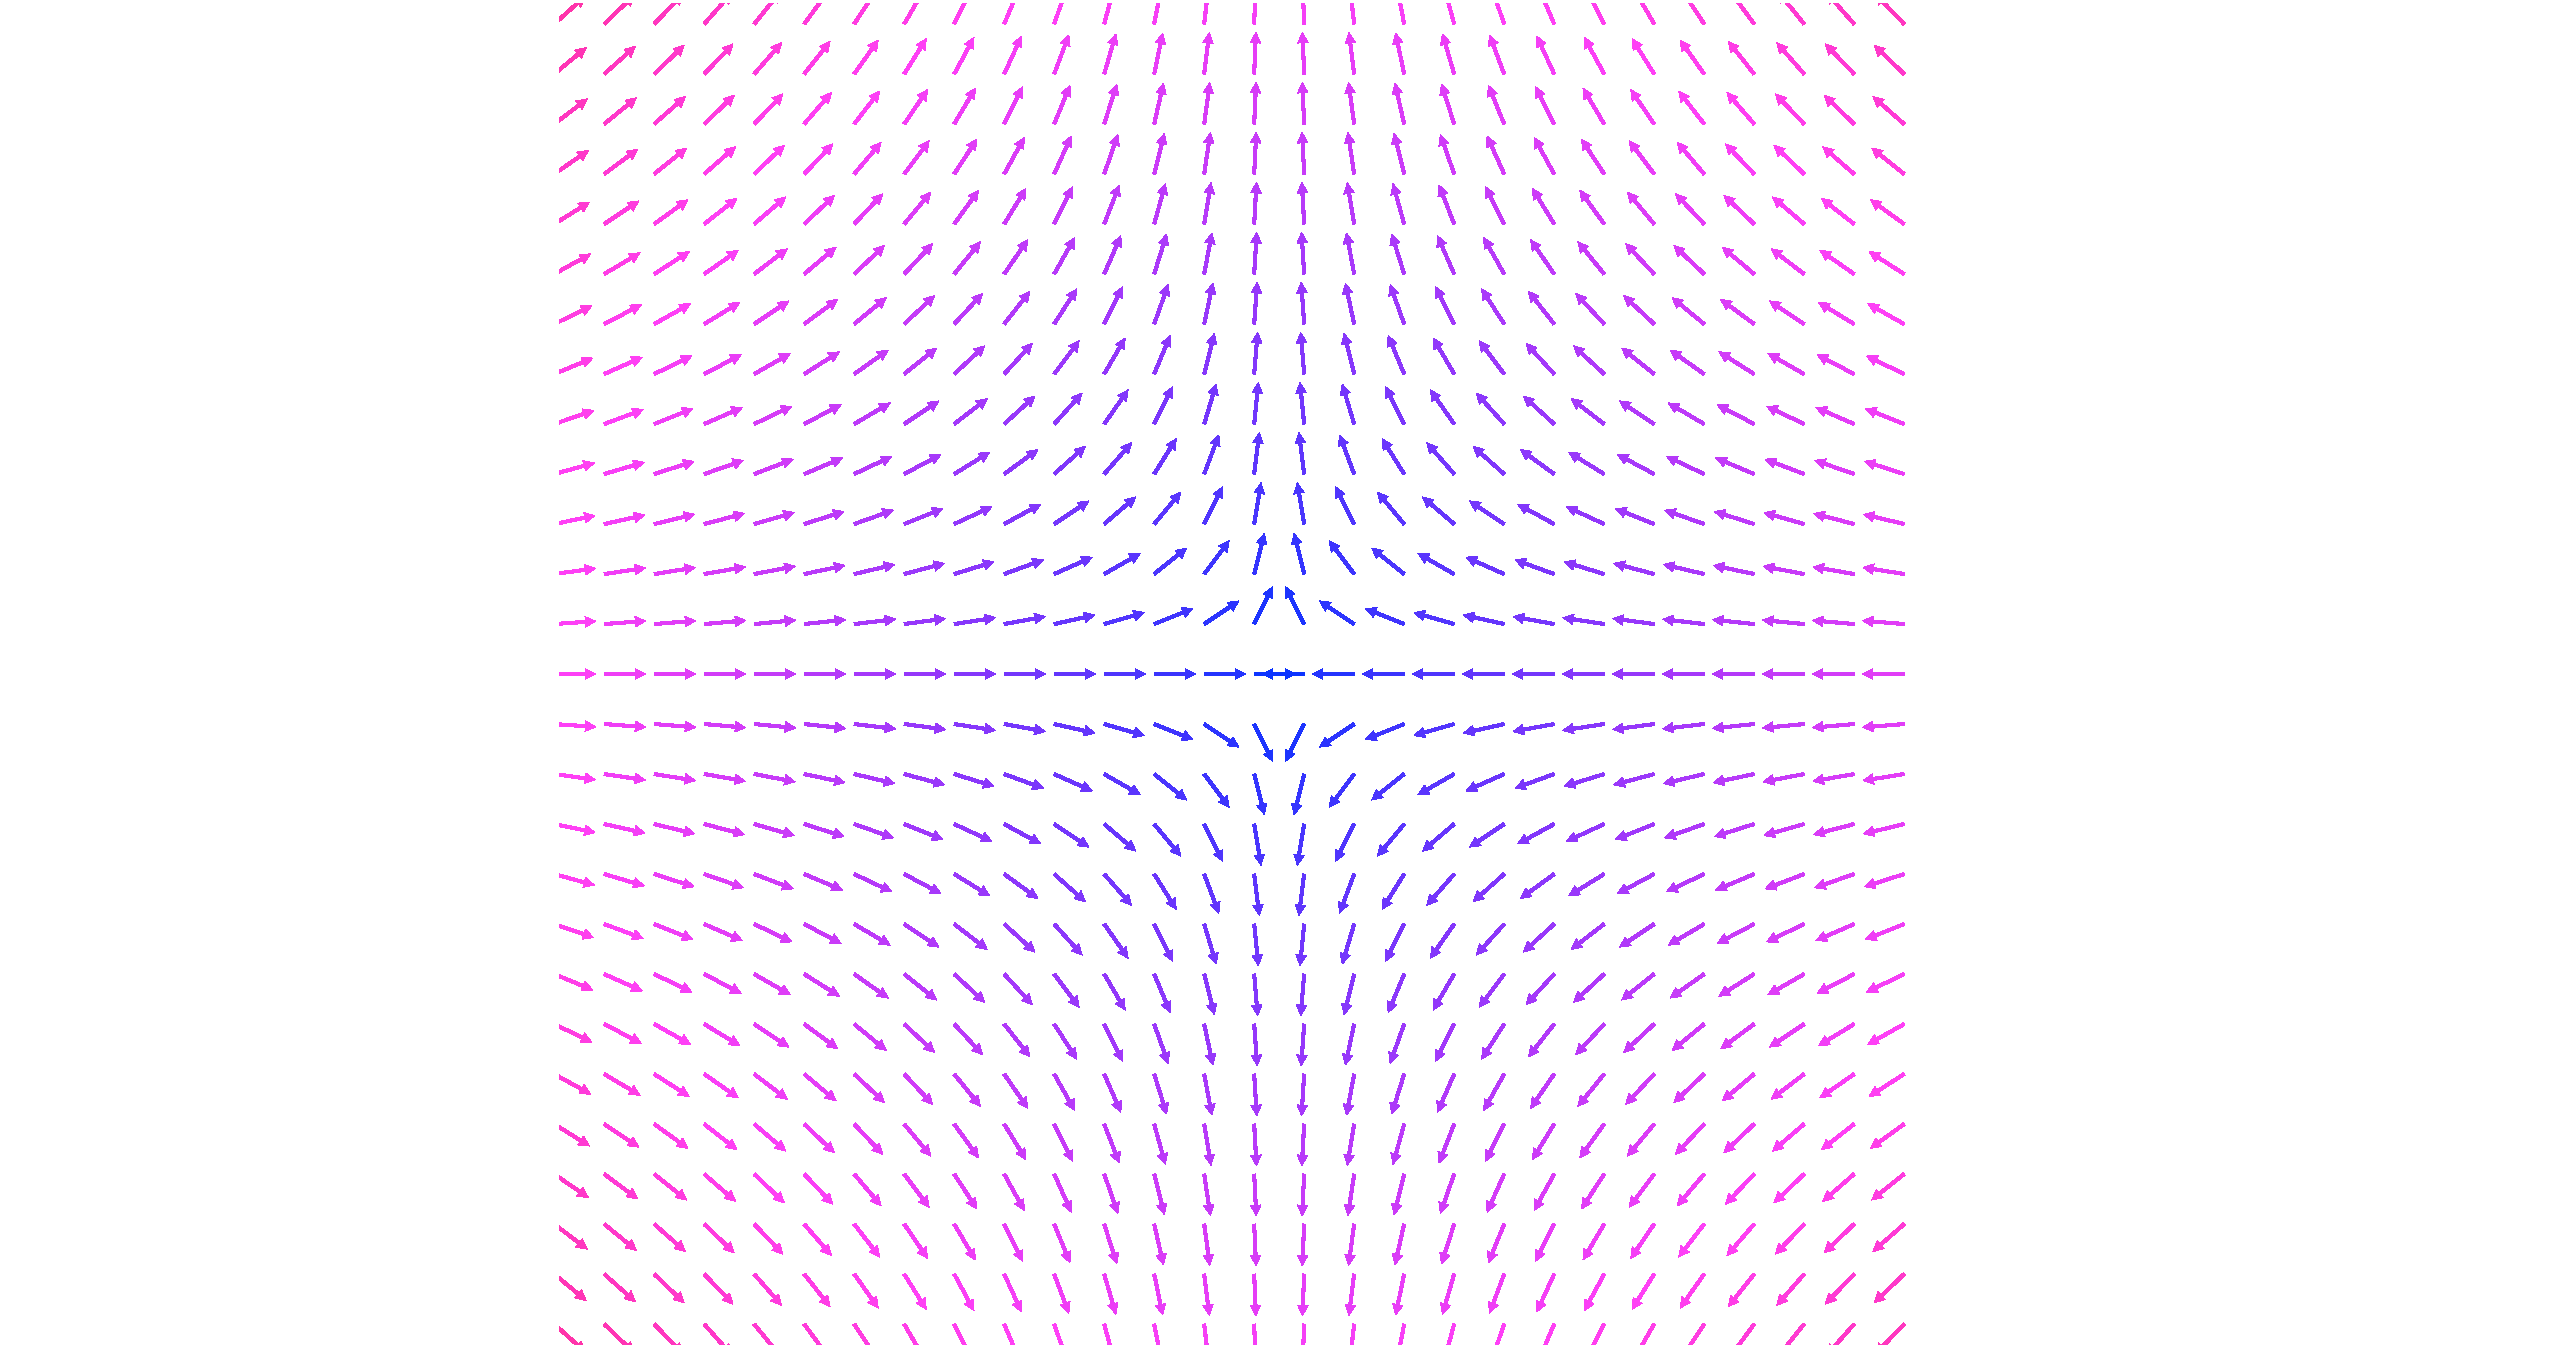
\includegraphics[width=65mm]{data/velocityfield3.pdf}
    & 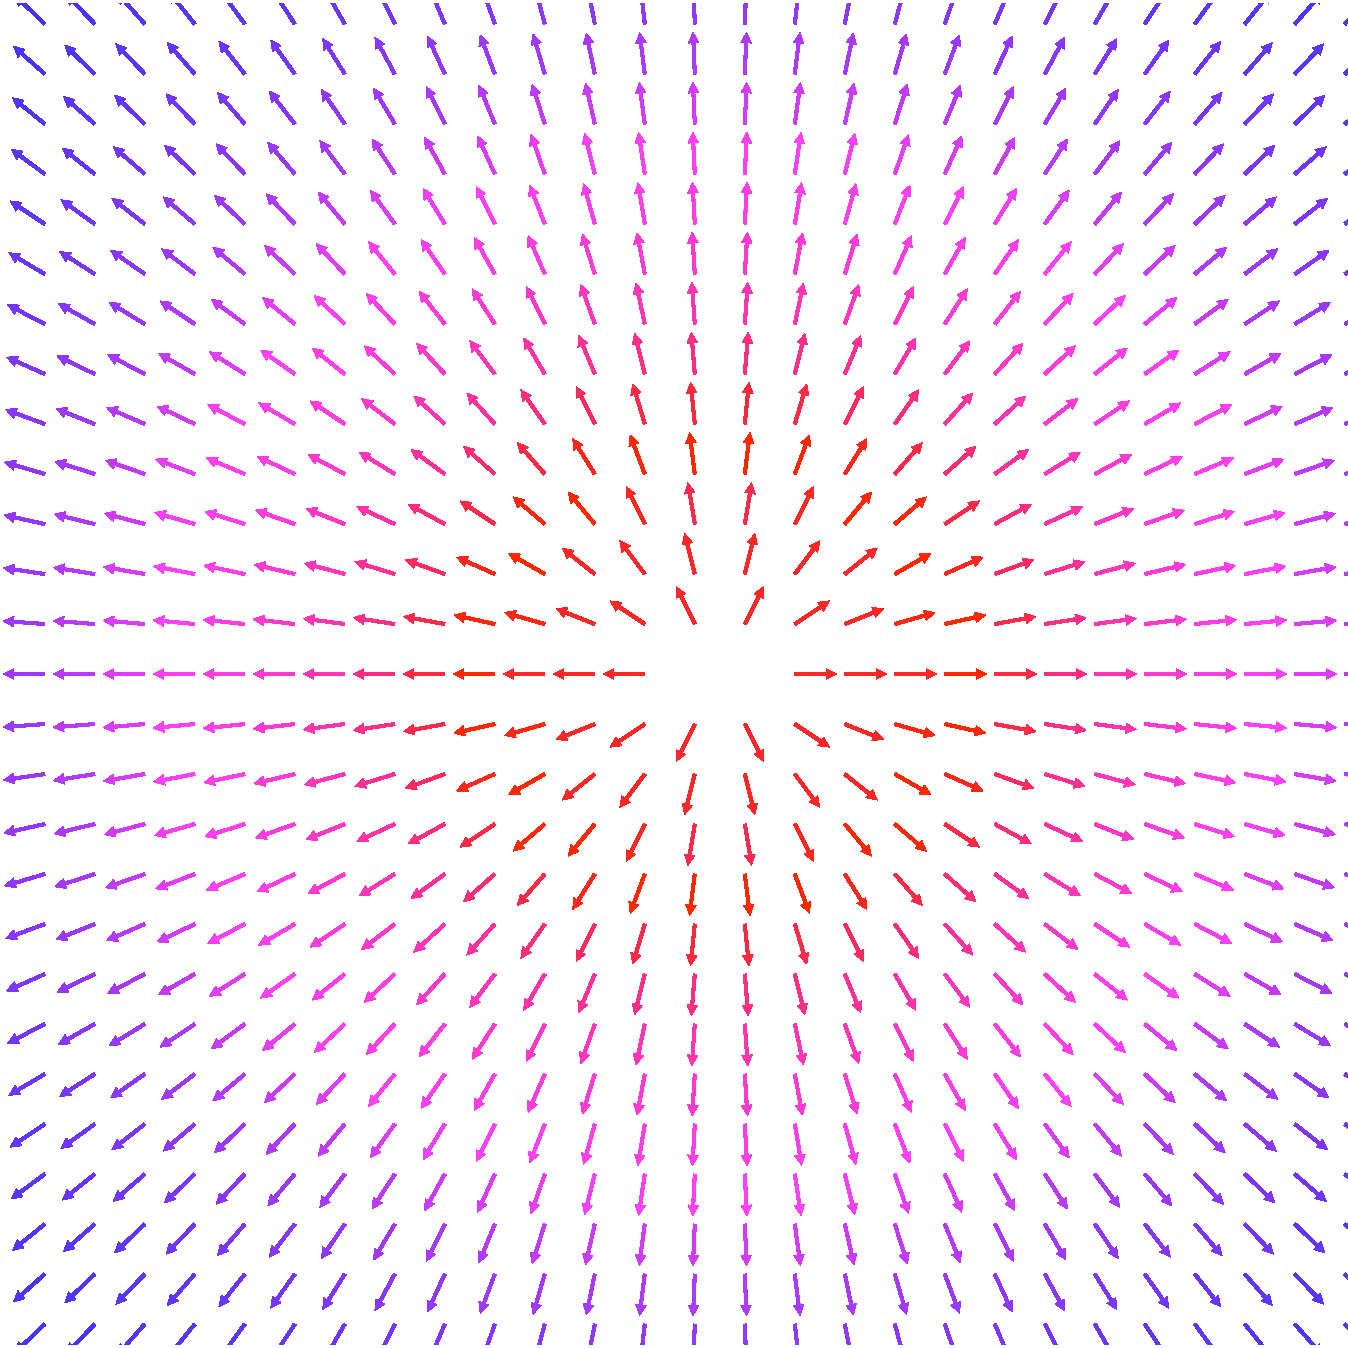
\includegraphics[width=65mm]{data/velocityfield4.pdf} \\
  \end{tabular}
  \caption{In each field, the blue vectors indicate low velocity,
    while the red vectors indicate high velocity. \textit{Top left:}
    fluid moving with a constant velocity toward the upper right.
    \textit{Top right:} fluid accelerating away from the origin.
    \textit{Bottom left:} fluid flowing in from the left and right,
    then flowing out toward the top and bottom. \textit{Bottom right:}
    fluid flowing away from the origin but slowing down.}
  \label{fig:velocity fields}
\end{figure}

The divergence of a velocity field at a particular point represents
the expansion (positive), compression (negative), or lack of either
(zero) of the fluid flow at that point.

For instance, the top-left field in figure \ref{fig:velocity fields}
shows a fluid with constant velocity. At any given point, the velocity
of fluid flowing in is the same as the velocity of fluid flowing out.
Everything balances, there is no compression or expansion, and there
is no divergence.

In contrast, the top-right field in figure \ref{fig:velocity fields}
shows a fluid that is accelerating. Since the velocity is greater
farther away from the origin, at any given point the fluid flowing in
from the origin will be moving slower than the fluid flowing out away
from the origin. Since the outflow is greater than the inflow, more
fluid must somehow be being added in order to make up the difference.
If we assume that the conservation of mass precludes fluid appearing
out of thin air, then the only way for less fluid to turn into more
fluid is if it expands. (In real life, this might be due to a change
in temperature or pressure. We don't really care what caused the
expansion, though -- just the fact that it is happening.) Thus, the
divergence is positive everywhere in the top-right field. (In fact,
the divergence is the \textit{same} everywhere in that field. The
important part is change in velocity, not just a field that ``looks''
like it is expanding, as is true near the center.)

Velocity fields can have zero divergence (be ``divergence free'') even
if they are not constant. For instance, the bottom-left field in
figure \ref{fig:velocity fields} has no divergence anywhere. You might
wonder how the velocity can flow toward the origin along the $x$-axis
without any compression, but note that unless the fluid is
\textit{precisely} on the $x$-axis it will break away and move up or
down. The fluid that \textit{is} precisely on the $x$-axis has an
infinitely small volume in any case, so it does not need to be
considered. Also, as the fluid moves up the $y$-axis its velocity
increases, but this effect is counterbalanced by more fluid moving
toward the $y$-axis, thus making the existing fluid flow faster.
Overall, everything cancels out and there is no divergence. (We'll see
the mathematics behind this momentarily -- it's not just visual!)

The bottom-right field in figure \ref{fig:velocity fields} is somewhat
counterintuitive: it looks like the fluid is expanding because it is
moving away from the origin, but in fact its divergence is
\textit{negative}! Why? Although the fluid is flowing outward, it is
also slowing down very quickly. This means that the amount of fluid
flowing out of any given point is \textit{less} than the amount of
fluid flowing into it. In general, it's quite difficult to tell what
the divergence of a field is just from a picture. (In particular, if
you don't know the magnitudes of the vectors, there's no way at all to
tell!) A radial velocity field can have positive, negative, or zero
divergence.

We have been discussing velocity fields in two dimensions, but of
course the same ideas apply for vector fields that do not represent
the velocity of a fluid and for vector fields in three or more
dimensions.

\subsubsection{Definition}
\label{sec:divergence definition}

In our intuitive discussion, we mentioned that divergence -- positive
or negative -- occurs when there is an imbalance in inflow and outflow
in a particular region. Inflow and outflow can be quantified using the
concept of \textit{flux}, which is defined based on either a line
integral or a surface integral depending on the number of dimensions.
In two dimensions, the net flux of $\vec{F}$ through a curve $C$ is
\[
  \int_C \vec{F} \cdot d\vec{s},
\]
and in three dimensions, the net flux of $\vec{F}$ through a surface
$S$ is
\[
  \iint_S \vec{F} \cdot d\vec{S}.
\]
In the first formula, $d\vec{s}$ is a normal vector to the curve,
pointing in the direction in which we are calculating flux and with a
magnitude corresponding to its length $ds$ on the curve. In the
second, $d\vec{S}$ is a normal vector to the surface, pointing in the
direction in which we are calculating flux and with a magnitude
corresponding to its surface area $dS$ on the surface.

We will be investigating flux out of \textit{closed} curves and
surfaces in our definition of divergence. (Positive divergence will
correspond to net flux out and negative divergence will correspond to
net flux in.) However, the flux out of any curve or surface will
depend on the value of the function at every point on the curve or
surface.

When we defined the derivative, we started with a \textit{non-local}
property, the slope of a secant line. This property depended on points
significantly far away from the point of interest. To obtain the
\textit{local} property of the slope of the tangent line -- which
depends only on points very, very (arbitrarily) close to the point of
interest -- we had to take a limit. Similarly, the flux through a
curve or surface is a non-local property, and we will have to take a
limit in order to obtain a local property -- the divergence, which
should only depend on points very, very close to the point of
interest. For instance, in the two-dimensional case we could try
\[
  \lim_{\text{Area}(C) \to 0} \int_C \vec{F} \cdot d\vec{s},
\]
where $\text{Area}(C)$ is the area \textit{enclosed} by $C$ (remember
that $C$ is a closed curve). Unfortunately, this limit is always zero
because as the area enclosed by the curve gets smaller, so will the
net flux in or out of it.

When we defined the derivative, we used the difference $f(x) - f(c)$.
However, just taking the limit as $x \to c$ would make this difference
go to zero, so we had to add a balancing factor of $x - c$ to the
denominator. Similarly, here we will have to add a balancing factor of
$\text{Area}(C)$ to the denominator. So a reasonable definition giving
the net amount of outward flux as a characteristic property of a
particular point is
\[
  \div \vec{F} = \lim_{\text{Area}(C) \to 0}
  \frac{\int_C \vec{F} \cdot d\vec{s}}{\text{Area}(C)}.
\]
In three dimensions, this would be
\[
  \div \vec{F} = \lim_{\text{Volume}(S) \to 0}
  \frac{\iint_S \vec{F} \cdot d\vec{S}}{\text{Volume}(S)},
\]
and the idea generalizes nicely to higher dimensions. These limits
give rise to the informal definitions of divergence as ``flux per unit
area'' or ``flux per unit volume'', just as the derivative is the
``change in $y$ per unit change in $x$''.

You may have wondered why we did not use arc length instead of
enclosed area, or surface area instead of enclosed volume. The problem
with these quantities is that they can be changed immensely without
changing the amount of net flux. You can see how to increase the arc
length of a contour without changing its net flux in figure
\ref{fig:ripple flux}.

\begin{figure}[htb!] \centering
  \begin{tikzpicture}

    \draw [gray!50] plot [smooth] coordinates
    {(1, 2.5) (3, 4.5) (3.1, 4.4) (1.08, 2.38)};

    \draw plot [smooth cycle] coordinates
    {(0, 0) (2, 1) (1, 2.5) (0.5, 4)
      (-2, 3.5) (-1.5, 2.5) (-1.5, 0.5)};

    \draw [->] (2, 3.5) ++(-0.6, 0.6) -- +(1.1, -1.1);
    \draw [->] (2.2, 3.7) ++(-0.6, 0.6) -- +(1.2, -1.2);
    \draw [->] (2.4, 3.9) ++(-0.5, 0.5) -- +(1.1, -1.1);

  \end{tikzpicture}
  \caption{The black contour represents a region which will have a
    certain amount of net flux. If the gray contour is added, the arc
    length of the contour will be increased greatly, but the flux will
    not change significantly since any flux in the region of the gray
    contour will just enter one side and exit the other -- the vector
    field does not have the chance to change significantly across the
    width of the gray contour.}
  \label{fig:ripple flux}
\end{figure}

Of course, we didn't give a specific reason why the formula takes the
particular form it does, but then again defining ``amount of net flux
as a function of position'' is a far more nebulous proposition than
defining ``slope of the tangent line as a function of position'',
which is quite straightforward. In the end, the reasonability of this
definition of divergence is tested by seeing if its behavior agrees
with what we would intuitively expect.

You will see in the next section that this definition gives a very
nice, concise formula for the divergence of a field.

\subsubsection{Definition with Partial Derivatives}
\label{sec:divergence definition with partial derivatives}

Let's derive a more straightforward formula for the divergence in two
dimensions. To evaluate the limit in the definition, we'll consider a
contour that is so small we can calculate the line integral directly.
Such a contour is shown in figure \ref{fig:divergence rectangle}.

\newsavebox{\divergencerectangle}
\savebox{\divergencerectangle}{
  \begin{tikzpicture}

    \draw (0, 0) node [below left] {$(x, y)$}
    -- (7, 0) node [below right] {$(x + \Delta x, y)$}
    node [midway, below] {$\vec{F} \approx \vec{F}(x, y)$}
    -- (7, 3) node [above right] {$(x + \Delta x, y + \Delta y)$}
    node [midway, right] {$\vec{F} \approx \vec{F}(x + \Delta x, y)$}
    -- (0, 3) node [above left] {$(x, y + \Delta y)$}
    node [midway, above] {$\vec{F} \approx \vec{F}(x, y + \Delta y)$}
    -- cycle node [midway, left] {$\vec{F} \approx \vec{F}(x, y)$};
    \foreach \x/\y in {0/0, 7/0, 7/3, 0/3} {
      \fill (\x, \y) circle (2pt);
    }

  \end{tikzpicture}
}

\begin{figure}[htb!] \centering
  \usebox{\divergencerectangle}
  \caption{A small contour that can be used in the definition of
    divergence (and curl; see page \pageref{sec:curl definition with
      partial derivatives}). The rectangle has a width of $\Delta x$
    and a height of $\Delta y$. We can approximate $\vec{F}$ as
    constant along each side, although a fully rigorous proof would
    not do so. The flux out of each side depends on the length of the
    side and the component of $\vec{F}$ normal to the side.}
  \label{fig:divergence rectangle}
\end{figure}

The contour used in the definition can be approximated as a rectangle.
The proof we are about to follow will work for any contour, but this
simplified version should make the idea clear. We want to find
\[
  \frac{\int_C \vec{F} \cdot d\vec{s}}{\text{Area}(C)}.
\]
The area enclosed by $C$ is easy to find using the coordinates on the
figure: it is simply $\Delta x \Delta y$. To find the net flux out of
$C$, we can look at each of the four sides individually and add their
flux together.

First, take the bottom side. We can assume that $\vec{F}$ is
relatively constant over such a short range ($\Delta x$), and say it
has the value of $\vec{F}(x, y)$ everywhere on the bottom side. Then,
since $\vec{F}$ is constant, we can compute the line integral
\[
  \int_{C_\text{bottom}} \vec{F}(x, y) \cdot d\vec{s}
\]
directly. Remember that $d\vec{s}$ is a normal vector pointing out of
the curve; for the bottom side we will have $d\vec{s} = -\jh \,dx$. We
will thus have
\[
  \int_{C_\text{bottom}} \big(F_x(x, y) \ih + F_y(x, y) \jh\big)
  \cdot \big(-\jh \,dx\big)
  = \int_x^{x + \Delta x} -F_y(x, y) \,dx
  = -F_y(x, y) \Delta x.
\]

You can (and should) compute the fluxes for the right, top, and left
sides as well. They are $F_x(x + \Delta x, y) \Delta y$,
$F_y(x, y + \Delta y) \Delta x$, and $-F_x(x, y) \Delta y$
respectively. We can find the net flux out of the contour by summing
all four of these numbers together:
\[
  \int_C \vec{F} \cdot d\vec{s}
  = F_x(x + \Delta x, y)\Delta y
  - F_x(x, y)\Delta y
  + F_y(x, y + \Delta y)\Delta x
  - F_y(x, y)\Delta x.
\]

Then, we can simply apply the definition:
\begin{align*}
  \div \vec{F}
  &= \lim_{\text{Area}(C) \to 0}
    \frac{\int_C \vec{F} \cdot d\vec{s}}{\text{Area}(C)} \\
  &= \lim_{\Delta x, \Delta y \to 0}
    \frac{
    F_x(x + \Delta x, y)\Delta y -
    F_x(x, y)\Delta y +
    F_y(x, y + \Delta y)\Delta x -
    F_y(x, y)\Delta x}
    {\Delta x \Delta y} \\
  &= \lim_{\Delta x, \Delta y \to 0}
    \left[\frac{
    F_x(x + \Delta x, y)\Delta y -
    F_x(x, y)\Delta y}
    {\Delta x \Delta y} +
    \frac{F_y(x, y + \Delta y)\Delta x -
    F_y(x, y)\Delta x}
    {\Delta x \Delta y}\right] \\
  &= \lim_{\Delta x \to 0}
    \left[\frac{
    F_x(x + \Delta x, y) -
    F_x(x, y)}
    {\Delta x}\right] +
    \lim_{\Delta y \to 0}
    \left[\frac{
    F_y(x, y + \Delta y) -
    F_y(x, y)}
    {\Delta y}\right] \\
  &= \frac{\partial F_x}{\partial x}
    + \frac{\partial F_y}{\partial y}.
\end{align*}

In the last step, we have simply used the definition of partial
derivative. You can do the same proof except with a rectangular prism
instead of a rectangle, and you will see that the divergence in three
dimensions is exactly analogous to the divergence in two dimensions:
\[
  \div \vec{F} =
  \frac{\partial F_x}{\partial x} +
  \frac{\partial F_y}{\partial y} +
  \frac{\partial F_z}{\partial z}.
\]

Recalling the symbolic convenience
\[
  \del =
  \frac{\partial}{\partial x} \ih +
  \frac{\partial}{\partial y} \jh +
  \frac{\partial}{\partial z} \kh,
\]
you can also write this as
\[
  \div \vec{F} = \del \cdot \vec{F}.
\]

\subsection{The Divergence Theorem}
\label{sec:divergence theorem}

\begin{prereq}
  Understand divergence (see section \ref{sec:divergence}), flux, and
  volume integrals.
\end{prereq}

The divergence theorem is a natural consequence of the definition of
divergence, expanded to a macroscopic scale (rather than the
microscopic scale used in the definition). In two dimensions, it
states that
\[
  \iint_R \div \vec{F} \,dA = \int_C \vec{F} \cdot d\vec{s},
\]
where $C$ is a closed contour that bounds the region $R$. In three
dimensions, it states that
\[
  \iiint_Q \div \vec{F} \,dV = \iint_S \vec{F} \cdot d\vec{S},
\]
where $S$ is a closed surface that bounds the region $Q$. Here,
$\div \vec{F}$ should be continuous. (There are some odd cases of
vector fields with non-continuous divergence that would otherwise
violate the divergence theorem.)

We will prove the two-dimensional case. First consider a region that
is split into two subregions, as shown in figure \ref{fig:divergence
  theorem}.

\begin{figure}[htb!] \centering
  \begin{tikzpicture}[scale=0.75]

    \draw plot [smooth cycle] coordinates {
      (0, 0) (3, -1) (2, 3) (3, 5)
      (0, 4) (-2, 5) (-4, 2) (-4, -1)};
    \draw (0, 0) -- (0, 4);
    \path (-2, 2) node {$A$};
    \path (1, 2) node {$B$};

  \end{tikzpicture}
  \caption{An arbitrary region $R$ divided into two subregions $A$ and
    $B$. The boundary line between the regions does not add any flux
    since the flux out of $A$ through the boundary will be exactly the
    same as the flux out of $B$ through the boundary, but with
    opposite sign.}
  \label{fig:divergence theorem}
\end{figure}

What is the net flux out of the region? It is the sum of the net
fluxes out of $A$ and $B$. All flux that exits $A$ through the
vertical line will just enter $B$, and vice versa. The flux along the
vertical line has the same magnitude but opposite sign in $A$ and $B$,
so when the two fluxes are added together this component will cancel
out. All that is left is the flux along the boundary of the region,
which means that the sum of the net fluxes out of $A$ and $B$ gives
the flux out of the total region they make up.

In general, a region can be divided into any number of subregions, and
the total flux out of the region can be found by adding together the
net fluxes out of each subregion. In addition, this reasoning will
also apply to three dimensions, where a region in space will be
divided into subregions divided by surfaces.

How does this help us prove the divergence theorem? Recall that the
definition of divergence is ``net flux out divided by area, for very
small area''. This could be written as
\[
  \div \vec{F} = \frac{d(\text{net flux out})}{dA}.
\]
To find the total flux out of a large number of these small regions,
we must multiply each of them by $dA$ and then add them all together.
[In other words,
$\iint_R d(\text{net flux out}) = \text{total flux out}$.] In fact,
this is exactly what the divergence theorem states:
\[
  \iint_R \underbrace
  {\div \vec{F} \,dA\vphantom{\int}}
  _{d(\text{net flux out})}
  = \underbrace{\int_C \vec{F} \cdot d\vec{s}}_\text{total flux out}.
\]

Of course, a similar proof can be followed in three or more
dimensions.

\subsection{The Curl}
\label{sec:curl}

\begin{prereq}
  Understand line integrals and partial derivatives.
\end{prereq}

\subsubsection{Intuition}
\label{sec:curl intuition}

The curl is an operation that takes a vector field $\vec{F}$ and
returns a different vector field, $\curl \vec{F}$.

Suppose again that $\vec{F}$ is the velocity field of a fluid (in
three dimensions), and suppose that we have placed a very small sphere
with a rough surface at the point of interest in this field. Suppose
further that we are somehow able to prevent this sphere from moving in
any direction but also allow it to \textit{rotate} in any direction
without resistance. (Never mind how!) For some velocity fields, the
motion of the fluid combined with the rough surface of the sphere will
cause it to rotate. The curl is directly related to the rotation of
the sphere.

But we want to be more precise than this. What is the most concise way
to describe the rotation of a sphere? The two things that need to be
specified are the axis of rotation and the rate of rotation
(revolutions per second, or degrees per second, or preferably radians
per second). That makes a vector (direction and magnitude)! The only
thing missing is specifying which way the rotation is -- clockwise or
counterclockwise. We will say that the vector shall be oriented in
such a way that when you look from the direction the vector is
pointing to, the sphere appears to be rotating counterclockwise. This
setup is illustrated in figure \ref{fig:curl sphere}.

\begin{figure}[htb!] \centering

  \tdplotsetmaincoords
  {0} % increase to look from below
  {0} % increase to look from the right
  \tdplotsetrotatedcoords
  {60}{60}{60}

  \begin{tikzpicture}[
    tdplot_rotated_coords,
    every pin edge/.style={black!65, thin, -}]

    \newcommand\sang{-12}
    \newcommand\eang{250}

    \tdplottransformmainscreen{0}{0}{0}

    \shade[tdplot_screen_coords, ball color = yellow]
    (\tdplotresx,\tdplotresy) circle (1);

    \draw [->, ultra thick] (\sang:1.25) arc (\sang:\eang:1.25);

    \draw [->, ultra thick] (0, 0, 1) -- (0, 0, 3)
    node [midway, pin={[pin distance=1cm]0:curl vector}] {};

    \draw [dashed] (0, 0, 1) -- (0, 0, 0) -- (50:1.25);
    \draw (0, 0, 0.25) -- ++(50:0.25) -- ++(0, 0, -0.25);

  \end{tikzpicture}
  \caption{The traditional way to describe the rotation of an object
    (in this case a sphere) using a single vector. This scheme is
    often referred to as the ``right-hand rule'', because if you curl
    the fingers of your right hand in the direction of rotation of the
    sphere, then your thumb will point in the direction of the curl
    (angular velocity) vector.}
  \label{fig:curl sphere}
\end{figure}

The rotating sphere analogy gives a nice way to visualize an arbitrary
component of the curl. In figure \ref{fig:curl sphere}, consider
passing a frictionless vertical rod through the sphere, so that it
could only rotate around a vertical axis. Then the sphere will have a
new ``rotation vector'', which will represent only the rotation about
a vertical axis. This vector will be the component of the
unconstrained rotation vector in the direction of the vertical axis.
We'll return to this way of finding a component of the curl
momentarily.

\subsubsection{Definition}
\label{sec:curl definition}

We saw that the gradient could be defined as the unique vector whose
components were given by a particular formula. (In the case of the
gradient, that formula was the directional derivative in the direction
of the component.) We defined the divergence using the limit of a line
integral. In our definition of the curl, we will combine both of these
strategies.

In the previous section, we saw that the component of the curl in a
particular direction was directly related to the angular velocity
(rate of rotation) of a rough-surfaced sphere constrained to rotate
about an axis in the direction of the component. All we have to do is
quantify this property. For simplicity, we will just consider a
cross-section of the sphere on the plane normal to the component in
which we are interested, which is a circle $C$. So given the curve $C$
and a velocity field $\vec{F}$, we want to find a number corresponding
to the tendency of the circle (sphere) to rotate counterclockwise
(positive) or clockwise (negative). This will be the magnitude of the
component of the curl vector pointing out of the page (see figure
\ref{fig:curl circle}) because we defined the vector as pointing in
the direction from which you can look to see the sphere (circle)
rotating counterclockwise.

\begin{figure}[htb!] \centering
  \begin{tikzpicture}

    \draw [
    decoration={
      markings,
      mark=at position 0.9 with {\arrow[scale=2.5]{>}}},
    postaction={decorate}]
    (0, 0) circle (2);

    \fill (45:2) circle (1.5pt);

    \draw [->] (45:2) -- +(135:2)
    node [midway, above right] {$d\vec{x}$};

    \draw [->] (45:2) -- +(-10:3)
    node [midway, above] {$\vec{F}$};

  \end{tikzpicture}
  \caption{The tangent vector $d\vec{x}$ and the velocity field
    $\vec{F}$ at one point along a contour. In this case, since
    $\vec{F}$ and $d\vec{x}$ are pointing in opposite directions,
    $\vec{F}$ would tend to rotate the contour clockwise -- the
    opposite direction of $d\vec{x}$. This idea can be quantified
    using the dot product $\vec{F} \cdot d\vec{x}$.}
  \label{fig:curl circle}
\end{figure}

We can quantify the tendency of the fluid flow $\vec{F}$ to make the
circle rotate by looking at each point on the circle individually and
summing the results (this is an integral). If $d\vec{x}$ is a tangent
vector that points in the counterclockwise direction along the circle,
as shown in figure \ref{fig:curl circle}, then the tendency of the
circle to rotate counterclockwise is maximized when $\vec{F}$ and
$d\vec{x}$ are parallel. The tendency is, of course, minimized when
the vectors are antiparallel (pointing in opposite directions). And
there is no tendency for the sphere to rotate if $\vec{F}$ and
$d\vec{x}$ are orthogonal. To be precise, the tendency to rotate
counterclockwise is given by $d\tau = \vec{F} \cdot d\vec{x}$, where
$\tau$ stands for tendency to rotate (or torque). The total torque is,
of course, given by
\[
  \tau = \int_C d\tau = \int_C \vec{F} \cdot d\vec{x}.
\]
This quantity is called the \textit{circulation} of $\text{F}$ around
$C$.

Note here that the differential vector is a \textit{tangent} vector to
the curve and not a normal vector as it was in the definition of flux.
(To be precise, the magnitude of $d\vec{x}$ is the arc length of its
small section of curve.) I have adopted the convention that $d\vec{s}$
and $d\vec{S}$ are normal vectors while $d\vec{x}$ is a tangent
vector. (In most sources, you will see $d\vec{n}$ and $d\vec{S}$ as
normal vectors, while $d\vec{s}$ is a tangent vector. I think this is
confusing. The important thing, of course, is to know what your
equations mean intuitively so that you are never confused by
notation!)

Naturally the torque on an object affects its rotation, but so does
its mass. Since our circular cross-section is a two-dimensional
figure, we'll assume its mass is proportional to its area. An object
with twice the mass is twice as hard to rotate, so the rotation, or
curl, of our circle will be inversely proportional to its area.
Therefore, we have the following formula:
\[
  \text{component of }\curl \vec{F}
  = \frac{\int_C \vec{F} \cdot d\vec{x}}{\text{Area}(C)}.
\]
Oops! Our curl depends on the size of the circle. We'll want to use an
arbitrarily small region, just as we did for gradient:
\[
  \text{component of }\curl \vec{F}
  = \lim_{\text{Area}(C) \to 0}
  \frac{\int_C \vec{F} \cdot d\vec{x}}{\text{Area}(C)}.
\]
Wow! Look how similar that is to the limit definition of divergence.
It should come as no surprise that just as the divergence is sometimes
called the flux per unit area, the curl is sometimes called the
circulation per unit area.

The most important difference is that curl, being a vector, is more
complicated than divergence in that its limit formula only gives one
component of the curl.

The curl is defined as the unique vector whose component in any
direction is given by the formula above, where $C$ is a contour in the
plane normal to the direction of the component. (The line integral
should also be oriented in a counterclockwise direction when viewed
from the direction in which the component is pointing.)

\subsubsection{Definition with Partial Derivatives}
\label{sec:curl definition with partial derivatives}

The curl is so analogous to the divergence that the derivation of a
formula for the curl in terms of partial derivatives is essentially
the same as the derivation for divergence, just using a slightly
different line integral. The only major difference is that we will
have to find the curl one component at a time, because its limit
definition only gives us one component. We will find the
$\kh$-component first. The figure from the divergence proof is
reprinted here for your convenience:

\begin{figure*}[htb!] \centering
  \usebox{\divergencerectangle}
\end{figure*}

Notice that in this figure the $\kh$ unit vector is pointing up out of
the page, and so the contour pictured is indeed normal to the
component we are interested in (the $\kh$-component). Of course, the
line integral should be evaluated in the counterclockwise direction.

This time, we must again evaluate the dot product in the line integral
for each of the four sides, except with $d\vec{x}$ instead of
$d\vec{s}$ (a tangent vector instead of a normal vector). For
instance, for the bottom side, $d\vec{x} = \ih \,dx$ and so
\[
  \int_{C_{\text{bottom}}}
  \big(F_x(x, y) \ih + F_y(x, y) \jh\big)
  \cdot \big(\ih \,dx\big)
  = \int_x^{x + \Delta x} F_x(x, y) \,dx
  = F_x(x, y)\Delta x.
\]
You should evaluate the line integrals for the other three sides. You
should get $F_y(x + \Delta x, y)\Delta y$,
$-F_x(x, y + \Delta y)\Delta x$, and $-F_y(x, y)\Delta y$ for the
right, top, and left sides respectively.

We can find the total circulation of $\vec{F}$ around $C$ by summing
these four components:
\[
  \int_C \vec{F} \cdot d\vec{x}
  = F_y(x + \Delta x, y)\Delta y
  - F_y(x, y)\Delta y
  + F_x(x, y)\Delta x
  - F_x(x, y + \Delta y)\Delta x.
\]
Then, we can simply apply the definition of the $\kh$-component of
curl:

\begin{align*}
  \curls_{\kh} \vec{F}
  &= \lim_{\text{Area}(C) \to 0}
    \frac{\int_C \vec{F} \cdot d\vec{x}}{\text{Area}(C)} \\
  &= \lim_{\Delta x, \Delta y \to 0}
    \frac{
    F_y(x + \Delta x, y)\Delta y -
    F_y(x, y)\Delta y +
    F_x(x, y)\Delta x -
    F_x(x, y + \Delta y)\Delta x}
    {\Delta x \Delta y} \\
  &= \lim_{\Delta x, \Delta y \to 0}
    \left[\frac{
    F_y(x + \Delta x, y)\Delta y -
    F_y(x, y)\Delta y}{\Delta x \Delta y} +
    \frac{F_x(x, y)\Delta x -
    F_x(x, y + \Delta y)\Delta x}
    {\Delta x \Delta y}\right] \\
  &= \lim_{\Delta x \to 0}
    \left[\frac{
    F_y(x + \Delta x, y) -
    F_y(x, y)}{\Delta x}\right]
    + \lim_{\Delta y \to 0}
    \left[\frac{
    F_x(x, y) -
    F_x(x, y + \Delta y)}
    {\Delta y}\right] \\
  &= \frac{\partial F_y}{\partial x}
    - \frac{\partial F_x}{\partial y}.
\end{align*}

Since this expression is quite a bit more complicated than the one for
divergence, here's an intuitive explanation. The circle we are
attempting to spin in the counterclockwise direction is shown in
figure \ref{fig:circle spin}.

\begin{figure}[htb!] \centering
  \begin{tikzpicture}

    \draw (0, 0) circle (1);
    \draw [->] (-1, -1.25) -- (1, -1.25);
    \draw [->] (-1, 1.25) -- (0.5, 1.25);
    \draw [->] (1.25, -1) -- (1.25, 1);
    \draw [->] (-1.25, -1) -- (-1.25, 0.5);

  \end{tikzpicture}
  \caption{An intuitive perspective on the conditions that will cause
    a disk to rotate counterclockwise. The vertical arrows represent
    the $y$ component of $\vec{F}$ as it varies with respect to $x$,
    while the horizontal arrows represent the $x$ component of
    $\vec{F}$ as it varies with respect to $y$.}
  \label{fig:circle spin}
\end{figure}

Each of the arrows along the side represents a component of the field
$\vec{F}$ that can spin the circle. Clearly, if we want to spin the
circle counterclockwise, the bottom arrow should be stronger than the
top arrow and the right arrow should be stronger than the left arrow.
This corresponds to the $x$ component of $\vec{F}$ decreasing as you
move upwards and the $y$ component of $\vec{F}$ increasing as you move
to the right. In other words, we want $\partial F_x/\partial y$ to be
negative and $\partial F_y/\partial x$ to be positive. This is exactly
the condition we need in order for the formula for the $\kh$-component
of the curl to work out positive (which means the circle is spinning
counterclockwise when viewed from above, the direction in which $\kh$
points).

You can follow essentially the same proof with rectangles oriented
normal to the $\ih$ and $\jh$ vectors to find the $\ih$- and
$\jh$-components of $\curl \vec{F}$. (This is a little tedious. The
most important part is the $\kh$-component, which gives you the curl
in two dimensions. Both the $\ih$ and $\jh$ components involve $z$,
which does not exist for a two-dimensional function.) Here is the full
formula for the curl:

\[
  \curl \vec{F}
  = \left(\frac{\partial F_z}{\partial y}
    - \frac{\partial F_y}{\partial z}\right) \ih
  + \left(\frac{\partial F_x}{\partial z}
    - \frac{\partial F_z}{\partial x}\right) \jh
  + \left(\frac{\partial F_y}{\partial x}
    - \frac{\partial F_x}{\partial y}\right) \kh.
\]

Since the derivations of the other two components are nearly identical
to the derivation for the $\kh$-component, the curl is actually quite
symmetric. In particular, consider the sequence
$(x, y, z, x, y, z, \dots)$. Find the letter corresponding to the
component you want ($x = \ih$, $y = \jh$, $z = \kh$) in this sequence.
Let the previous letter in the sequence be $a$ and the letter before
that be $b$. Then the relevant component of the curl is
\[
  \frac{\partial F_a}{\partial b} - \frac{\partial F_b}{\partial a}.
\]
Nevertheless, this is quite an ugly formula. But it just so turns out
that this formula is \textit{also} given by the expression
\[
  \curl \vec{F} = \del \times \vec{F} = \begin{vmatrix}
    \ih & \jh & \kh \\
    \frac{\partial}{\partial x} &
    \frac{\partial}{\partial y} &
    \frac{\partial}{\partial z} \\
    F_x & F_y & F_z \\
  \end{vmatrix}.
\]

It's amazing how pretty a bit of notation can make things! Go ahead
and work out the cross product -- you should get the formula given
above.

\subsection{Green's Theorem}
\label{sec:greens theorem}

\begin{prereq}
  Understand the divergence theorem (see section \ref{sec:divergence
    theorem}) and curl (see section \ref{sec:curl}).
\end{prereq}

Green's theorem is so analogous to the divergence theorem in two
dimensions that its proof hardly needs any introduction. By the way,
just as $\div \vec{F}$ must be continuous for the divergence theorem
to apply, $\curl \vec{F}$ must be continuous for Green's theorem to
apply. A particular function where this restriction ends up being
important is discussed in section \ref{sec:no curl caveat}.

\renewcommand{\arraystretch}{2}
\begin{longtable}{|P{0.47\textwidth}|P{0.47\textwidth}|}

  \hline

  Divergence theorem in two dimensions &
  Green's theorem \\

  \hline

  We want to prove
  \[
    \iint_R \div \vec{F} \,dA = \int_C \vec{F} \cdot d\vec{s}.
  \]
  Remember that $d\vec{s}$ is a \textit{normal} vector. &

  We want to prove
  \[
    \iint_R \curl \vec{F} \cdot \kh \,dA
    = \int_C \vec{F} \cdot d\vec{x}.
  \]
  Remember that $d\vec{x}$ is a \textit{tangent} vector. \\

  When we divide a region into two subregions, the net flux out of the
  region is equal to the sum of the net fluxes out of each of the two
  subregions, because any flux along the boundary line will be equal
  and opposite for the two subregions. &

  When we divide a region into two subregions, the circulation around
  the region is equal to the sum of the circulations around each of
  the two subregions, because any circulation along the boundary line
  will be equal and opposite for the two subregions. \\

  The definition of divergence is ``net flux out divided by area, for
  very small area''. This could be written as
  \[
    \div \vec{F} = \frac{d(\text{net flux out})}{dA}.
  \] &

  The definition of the $\kh$-component of curl is ``circulation
  divided by area, for very small area.'' This could be written as
  \[
    \curl \vec{F} \cdot \kh = \frac{d(\text{circulation})}{dA}.
  \] \\

  To find the total flux out of a large number of these small regions,
  we must multiply each of them by $dA$ and then add them together. In
  fact, this is exactly what the divergence theorem states:
  \[
    \iint_R \underbrace{\div \vec{F} \,dA
      \vphantom{\int}}_{d(\text{net flux out})}
    = \underbrace{\int_C \vec{F} \cdot d\vec{s}}
    _\text{total flux out}.
  \] &

  To find the total circulation around a large number of these small
  regions, we must multiply each of them by $dA$ and then add them
  together. In fact, this is exactly what Green's theorem states:
  \[
    \iint_R \underbrace{\curl \vec{F}
      \cdot \kh \,dA\vphantom{\int}}
    _{d(\text{circulation})}
    = \underbrace{\int_C \vec{F} \cdot d\vec{x}}
    _\text{circulation}.
  \] \\
  \hline
\end{longtable}

Let's clear up some technical details. Why did we have to choose the
$\kh$-component of the curl? We defined the curl using a limit
definition analogous to the limit definition for divergence. However,
this limit definition only gave one component of the curl. Which one?
The component must be normal to the plane of the contour and oriented
such that looking from the direction in which it is pointing will make
the line integral counterclockwise. The $\kh$ unit vector is normal to
the $xy$-plane that contains the contour, and it points out of the
paper. So as long as we take the line integral in the counterclockwise
direction, we can just substitute $\div \vec{F}$ with
$\curl \vec{F} \cdot \kh$ when proving Green's theorem by analogy.

\subsection{Stokes' Theorem}
\label{sec:stokes theorem}

\begin{prereq}
  Understand Green's theorem (see section \ref{sec:greens theorem})
  and surface integrals.
\end{prereq}

Stokes' theorem is a straightforward generalization of Green's theorem
to arbitrary surfaces in space rather than just flat regions in the
plane, just as the gradient theorem is a generalization of the
fundamental theorem of calculus to arbitrary curved paths rather than
just straight lines.

In Green's theorem, our circulation was within the $xy$-plane, so we
needed the $\kh$-component of the curl because it was normal to the
$xy$-plane. For an arbitrary surface, the principle remains the same
except that we need the component of the curl normal to the surface.
Thus, the equation will change from
\[
  \iint_R \curl \vec{F} \cdot \kh \,dA
  = \int_C \vec{F} \cdot d\vec{x}
\]
to
\[
  \iint_R \curl \vec{F} \cdot \vec{n} \,dS
  = \iint_R \curl \vec{F} \cdot d\vec{S}
  = \int_C \vec{F} \cdot d\vec{x},
\]
where $R$ can now be an arbitrary region in space (well, sort of -- no
spheres [which don't have edges] or M\"obius strips [which don't have
proper unit normal vectors $\vec{n}$] please!) bounded by the closed
contour $C$.

Note that the orientation of the line integral, as always, matters. In
particular, it should be oriented counterclockwise when you are
looking from the direction in which the normal vectors $d\vec{S}$ to
the surface are pointing. Also, $\curl \vec{F}$ should be continuous
for Stokes' theorem, just like for Green's theorem.

\subsubsection{The Divergence of the Curl}
\label{sec:divergence of curl}

\begin{prereq}
  Understand Stokes' theorem (see section \ref{sec:stokes theorem})
  and the divergence theorem (see section \ref{sec:divergence
    theorem}).
\end{prereq}

If you compute the expression $\div \curl \vec{F}$ and use the
equality of mixed partials, you will see that it always equals $0$.
(Try it!) That is, the curl has no divergence. But computing partial
derivatives is really the most unintuitive way possible to prove this
fact, especially given that the equality of mixed partials has no
easily accessible graphical interpretation that I have been able to
find.

However, Stokes' theorem and the divergence theorem can be used
together in a creative way to prove the same thing. We will start with
a justification for one of the steps in the proof. Suppose that you
know that $f(x)$ is a continuous function and also that
$\int_a^b f(x) \,dx = 0$ for every possible $a$ and $b$. You can then
conclude that $f(x) = 0$ always. (Convince yourself of this.)
Similarly, if you know that $f(x, y, z)$ is a continuous function and
also that $\iiint_Q f(x, y, z) \,dV = 0$ for every possible region
$Q$, you can then conclude that $f(x, y, z) = 0$ always.

Now for the actual proof. Consider the scalar field
$f(x, y, z) = \div \curl \vec{F}(x, y, z)$, where $\vec{F}$ is any
vector field. Suppose we are given an arbitrary region in space $Q$.
Then according to the divergence theorem in three dimensions,
\[
  \iiint_Q \div \curl \vec{F} \,dV
  = \iint_S \curl \vec{F} \cdot d\vec{S},
\]
where $S$ is the closed surface that bounds $Q$. At this point, it
will be useful to picture a region in space that you can easily divide
into a ``top half'' and ``bottom half'', such as a sphere. Draw an
arbitrary contour dividing the surface into these two halves. (Of
course, it does not matter what contour you pick. But it will be
easier to keep track of which vectors are going which direction if
both you and I are talking about the same halves of your surface.) The
surface integral can then be divided into two:
\[
  \iint_S \curl \vec{F} \cdot d\vec{S}
  = \iint_{S_\text{top}} \curl \vec{F} \cdot d\vec{S}
  + \iint_{S_\text{bottom}} \curl \vec{F} \cdot d\vec{S}.
\]
We can now apply Stokes' theorem to both of these now non-closed
surfaces. For the top half:
\[
  \iint_{S_\text{top}} \curl \vec{F} \cdot d\vec{S}
  = \int_C \curl \vec{F} \cdot d\vec{x},
\]
where $C$ is oriented counterclockwise because the normal vector is
pointing out and up. Since both halves of the surface are bounded by
the same contour, both surface integrals are equal to the same line
integral -- except that the orientation of the curve is the opposite!
When you look from below, the normal vector is again outwards and
pointing toward you, so the line integral is oriented
counterclockwise. But since you are looking from below, the line
integral is actually in the opposite direction to the original one.
Since reversing the direction of a line integral reverses its sign, we
have
\begin{align*}
  \iiint_Q \div \curl \vec{F} \,dV
  &= \iint_S \curl \vec{F} \cdot d\vec{S} \\
  &= \iint_{S_\text{top}} \curl \vec{F} \cdot d\vec{S}
    + \iint_{S_\text{bottom}} \curl \vec{F} \cdot d\vec{S} \\
  &= \int_C \curl \vec{F} \cdot d\vec{x}
    - \int_C \curl \vec{F} \cdot d\vec{x} \\
  &= 0.
\end{align*}
According to our earlier discussion, since the integral of
$f(x, y, z) = \div \curl \vec{F}(x, y, z)$ is $0$ over any region
whatsoever, we must have $\div \curl \vec{F} = 0$ everywhere, which
was to be demonstrated.

\subsection{Conservative Vector Fields}
\label{sec:conservative vector fields}

\begin{prereq}
  Understand the gradient theorem (see section \ref{sec:gradient
    theorem}) and Stokes' theorem (see section \ref{sec:stokes
    theorem}).
\end{prereq}

Vector fields (in both two and three dimensions) can have many
properties -- for instance, being divergence free, curl free,
differentiable, and so on. One of the most important properties of a
vector field is whether it is \textit{conservative}. There are quite a
few properties associated with conservative vector fields, and in this
section we explore each of those properties.

\subsubsection{Path Independence}
\label{sec:path independence}

The definition of \textit{conservative} is \textit{path independent}.
These two terms are completely equivalent. But of course now we need
to define what path independent means. If a vector field is path
independent, then for any two points $\vec{a}$ and $\vec{b}$, any line
integral between those two points will have the same value. For
instance, the vector field $\vec{F} = x \ih + y \jh$ is path
independent. This means that the line integrals along the four paths
pictured in figure \ref{fig:path independence} all have the same
value.

\begin{figure}[htb!] \centering
  \begin{tikzpicture}
    \begin{axis}[
      axis lines=middle,
      x axis line style={<->},
      y axis line style={->},
      xtick={1},
      ytick={1},
      unit vector ratio*=1 1,
      enlargelimits=true,
      width=12cm,
      clip=false]

      \addplot[smooth, domain=0:1] {x}
      node[pos=0.5, pin={[pin distance=1cm]-45:$y = x$}] {};

      \addplot[smooth, domain=0:1] {x*x}
      node[pos=0.8, pin={[pin distance=1cm]0:$y = x^2$}] {};

      \addplot[smooth, domain=0:1, variable=\t] ({-sin(270*t)}, t)
      node[pos=0.5, pin={
        [pin distance=1cm]135:$x =
        -\sin\left(\frac{3\pi}{2}y\right)$}] {};

      \addplot[domain=0:1, samples=3] {abs(x+0.5)-abs(x-0.5)}
      node[pos=0.6, pin={[pin distance=1cm]110:$y = 2x$}] {}
      node[pos=0.8, pin={[pin distance=0.5cm]90:$y = 1$}] {};

      \addplot[thick, -stealth, samples=2, domain=0.25:0.75,
      quiver={u=1, v=1, scale arrows=0.01}] {x};

      \addplot[thick, -stealth, samples=2, domain=0.25:0.75,
      quiver={u=1, v=2*x, scale arrows=0.01}] {x*x};

      \addplot[thick, -stealth, samples=2, domain=0.25:0.7,
      variable=\t, quiver={u=-1.5*pi*cos(270*t), v=1, scale
        arrows=0.005}] ({-sin(270*t)}, t);

      \addplot[thick, -stealth, samples=2, domain=0.25:0.75,
      quiver={u=1, v=(x<0.5)*2, scale arrows=0.01}]
      {abs(x+0.5)-abs(x-0.5)};


      \addplot[mark=*, mark size=1.5pt] coordinates {(0, 0) (1, 1)};

    \end{axis}

  \end{tikzpicture}
  \caption{Four paths from $\vec{a} = (0, 0)$ to $\vec{b} = (1, 1)$ in
    the vector field $\vec{F} = x \ih + y \jh$, all of which have the
    same value: $1$. The fact that all four of these integrals are the
    same does not mean that $\vec{F}$ is conservative, but it would be
    enough to make a reasonable hypothesis. You only need to find one
    integral with a different value to show that a vector field is not
    conservative, however.}
  \label{fig:path independence}
\end{figure}

You should try computing these integrals; you will find that
\begin{align*}
  \int_C \left(x \ih + y \jh\right) \cdot d\vec{x}
  &= \int_0^1 2t \,dt \\
  &= \int_0^1 2t^3 + t \,dt \\
  &= \int_0^1 \left[\frac{3\pi}{2} \sin\left(\frac{3\pi}{2}t\right)
    \cos\left(\frac{3\pi}{2}t\right) + t\right] \,dt \\
  &= \int_0^{1/2} 5t \,dt + \int_{1/2}^1 t \,dt \\
  &= 1.
\end{align*}

Of course, just because four line integrals between two points have
the same value does not mean that \textit{every} line integral will be
the same for \textit{any} given pair of two points. Later, we will see
how to easily determine whether a vector field is path independent
(conservative) without computing an uncountably infinite number of
line integrals.

It is, however, much easier to show that a vector field is path
dependent. You just have to find two paths between the same two points
whose line integrals are different. For instance, for the field
$\vec{F} = -y \ih + x \jh$, the line integrals corresponding to the
two paths shown in figure \ref{fig:path dependence} have different
values:
\begin{align*}
  \int_{C_1} \left(-y \ih + x \jh\right)
  \cdot \left(dx \ih + dy \jh\right)
  &= \int_0^\pi \cos^2 \theta + \sin^2 \theta \,d\theta = \pi \\
  \int_{C_2} \left(-y \ih + x \jh\right)
  \cdot \left(dx \ih + dy \jh\right)
  &= \int_0^\pi -\cos^2 \theta - \sin^2 \theta \,d\theta = -\pi
\end{align*}

Try finding these integrals yourself. Your results should verify that
the vector field $\vec{F}$ is \textit{nonconservative}.

\begin{figure}[htb!] \centering
  \begin{tikzpicture}[scale=3]

    \draw [<->] (-1.2, 0) -- (1.2, 0);
    \draw [<->] (0, -1.2) -- (0, 1.2);

    \draw [decoration={
      markings,
      mark=between positions 0.25 and 0.75 step 0.5 with
      {\arrow[scale=1.5]{stealth}}},
    postaction={decorate}]
    (1, 0) node[above right] {$(1, 0)$}
    arc (0:180:1) node[midway, above right]
    {$(0, 1)$} node[pos=0.2, pin={[pin distance=1cm]30:$C_1$}] {};

    \draw [decoration={
      markings,
      mark=between positions 0.25 and 0.75 step 0.5 with
      {\arrow[scale=1.5]{stealth}}},
    postaction={decorate}]
    (1, 0) arc (0:-180:1) node[below left, midway] {$(0, -1)$}
    node[below left] {$(-1, 0)$}
    node[pos=0.8, pin={[pin distance=1cm]-150:$C_2$}] {};

    \fill (1, 0) circle (0.5pt);
    \fill (-1, 0) circle (0.5pt);

  \end{tikzpicture}
  \caption{Two paths between $\vec{a} = (1, 0)$ and
    $\vec{b} = (-1, 0)$ in the vector field $\vec{F} = -y \ih + x \jh$
    with different values. Of course, there may be other paths between
    $\vec{a}$ and $\vec{b}$ with the same values as one of these
    paths, but this is irrelevant: \textit{every} path must give the
    same value in order for $\vec{F}$ to be considered conservative.}
  \label{fig:path dependence}
\end{figure}

\subsubsection{Potential Functions}
\label{sec:potential functions}

The \textit{potential function} of a vector field $\vec{F}$ is a
scalar field $f$ such that $\grad f = \vec{F}$. It is the
multivariable version of an antiderivative (a function $G$ such that
$G' = g$). Some vector fields have potential functions and some do
not. For instance, $\vec{F} = x \ih + y \jh$ has the potential
function $f = \frac{1}{2}x^2 + \frac{1}{2}y^2$ (check this), while
$\vec{F} = -y \ih + x \jh$ does not have any potential function. In
fact, a vector field has a potential function if and only if it is
conservative (path independent). We can prove this by first showing
that if a vector field has a potential function then it must be path
independent, and then showing that if a vector field is path
independent then it must have a potential function.

The first part of the proof is easy. If $\vec{F}$ has a potential
function (that is, if $\vec{F} = \grad f$) then according to the
gradient theorem,
\[
  \int_\vec{a}^\vec{b} \vec{F} \cdot d\vec{x}
  = \int_\vec{a}^\vec{b} \grad f \cdot d\vec{x}
  = f(\vec{b}) - f(\vec{a})
  = \text{constant}
\]
for \textit{any path} between $\vec{a}$ and $\vec{b}$. Therefore,
$\vec{F}$ is path independent.

The second part is slightly more nuanced. Given that $\vec{F}$ is path
independent, we must find a potential function $f$ such that
$\grad f = \vec{F}$. In one dimension, the function
\[
  G(x) = \int_a^x g(t) \,dt
\]
is an antiderivative of $g(x)$ for any $a$ according to the second
fundamental theorem of calculus. Luckily, we can extend this almost
directly to multiple dimensions: the function
\[
  f(\vec{x}) = \int_\vec{a}^\vec{x} \vec{F}(\vec{z}) \cdot d\vec{z}
\]
($\vec{z}$ has nothing to do with the $z$-axis; it is just a
convenient letter) is a potential function of $\vec{F}$ for any
$\vec{a}$ (assuming that $\vec{F}$ is path independent, because if it
were not we would have to explicitly give a path for the integral). In
any case, we can show that the gradient of this function is
$\vec{F}(\vec{x})$ by considering two different paths from $\vec{a}$
to $\vec{x}$. (To have a comprehensible diagram, we're assuming a
two-dimensional space. In a three-dimensional space, you would have to
consider three different paths.) These paths are shown in figure
\ref{fig:potential function}. (We'll say that
$\vec{a} = a_x \ih + a_y \jh$ and $\vec{x} = x \ih + y \jh$.)

\begin{figure}[htb!] \centering
  \begin{tikzpicture}[scale=3]

    \begin{scope}
      \fill (0, 0) circle (0.5pt) (0, 1)
      circle (0.5pt) (1, 1) circle (0.5pt);

      \draw [decoration={
        markings,
        mark=at position 0.25 with {\arrow[scale=1.5]{stealth}},
        mark=at position 0.75 with {\arrow[scale=1.5]{stealth}}},
      postaction={decorate}]
      (0, 0) node[below left] {$(a_x, a_y)$}
      -- (0, 1) node[above left] {$(a_x, y)$}
      -- (1, 1) node[above right] {$(x, y)$};
    \end{scope}
    \begin{scope}[xshift=2cm]
      \fill (0, 0) circle (0.5pt) (1, 0)
      circle (0.5pt) (1, 1) circle (0.5pt);

      \draw [decoration={
        markings,
        mark=at position 0.25 with {\arrow[scale=1.5]{stealth}},
        mark=at position 0.75 with {\arrow[scale=1.5]{stealth}}},
      postaction={decorate}]
      (0, 0) node[below left] {$(a_x, a_y)$}
      -- (1, 0) node[below right] {$(x, a_y)$}
      -- (1, 1) node[above right] {$(x, y)$};
    \end{scope}

  \end{tikzpicture}
  \caption{Two equivalent ways of computing the potential function $f$
    we have constructed. Of course, since $\vec{F}$ is path
    independent, you can take any path from $\vec{a}$ to $\vec{x}$ and
    get the same value, but these two particular paths make it much
    easier to find the partial derivatives of $f$ with respect to $x$
    and $y$.}
  \label{fig:potential function}
\end{figure}

Because $\vec{F}$ is path independent, both of the line integrals
pictured in figure \ref{fig:potential function} must have the same
value and must also therefore have the same partial derivatives in
both directions. So, we can find $\partial f/\partial x$ from the
left-hand diagram and $\partial f/\partial y$ from the right-hand
diagram.

For the left-hand contour,
\[
  f(\vec{x})
  = \int_{a_y}^y F_y(a_x, z) \,dz + \int_{a_x}^x F_x(z, y) \,dz
\]
and
\[
  \frac{\partial f(\vec{x})}{\partial x}
  = \frac{\partial}{\partial x} \int_{a_y}^y F_y(a_x, z) \,dz
  + \frac{\partial}{\partial x} \int_{a_x}^x F_x(z, y) \,dz
  = 0 + F_x(x, y)
  = F_x
\]
by recognizing that the first half of the integral does not depend on
$x$ and using the second fundamental theorem of calculus on the second
half of the integral. For the right-hand contour,
\[
  f(\vec{x})
  = \int_{a_x}^x F_x(z, a_y) \,dz + \int_{a_y}^y F_y(x, z) \,dz
\]
and
\[
  \frac{\partial f(\vec{x})}{\partial y}
  = \frac{\partial}{\partial y} \int_{a_x}^x F_x(z, a_y) \,dz
  + \frac{\partial}{\partial y} \int_{a_y}^y F_y(x, z) \,dz
  = 0 + F_y(x, y)
  = F_y
\]
by recognizing that the first half of the integral does not depend on
$y$ and using the second fundamental theorem of calculus on the second
half of the integral. So,
\[
  \grad f
  = \frac{\partial f}{\partial x} \ih
  + \frac{\partial f}{\partial y} \jh
  = F_x \ih + F_y \jh
  = \vec{F}.
\]
This proves that if a vector field is path-independent (conservative),
then it must have a potential function. Since we already proved the
converse, these two conditions are entirely equivalent.

\subsubsection{The Conservation of Energy}
\label{sec:conservation of energy}

At this point, we should discuss some nomenclature. Why are
path-independent vector fields called ``conservative''? Why is the
anti-gradient called a ``potential function''?

The answers to both of these questions lie in physics -- and more
specifically, in \textit{energy}. What is energy? You will find a wide
range of unsatisfying and sneakily worded answers from various
sources, but really the answer is quite simple: fundamentally, energy
is \textit{movement}. The only ``real'' type of energy is kinetic
energy. Specifically, an object with a mass $m$ moving at a speed of
$v$ is defined to have a kinetic energy of
\[
  K = \frac{1}{2}mv^2.
\]
Why this definition? It turns out that this particular definition is
related very closely to another definition: that of \textit{work}.
When a force $\vec{F}$ acts on an object moving along the path $C$,
the work done by that force on the object is defined to be
\[
  W = \int_C \vec{F} \cdot d\vec{x}.
\]
We can prove what is called the \textit{work-kinetic energy theorem}:
\[
  W = \Delta K.
\]
Over any given time interval, the change in kinetic energy of an
object with one force acting on it is equal to the work done by that
force. The proof is just some simple but rather sneaky manipulations
of the variables in the definition of work:
\begin{align*}
  W = \int_\vec{a}^\vec{b} \vec{F} \cdot d\vec{x}
  &= \int_{t_a}^{t_b} m\vec{a} \cdot \frac{d\vec{x}}{dt} dt \\
  &= \int_{t_a}^{t_b} m\frac{d\vec{v}}{dt} \cdot \vec{v} \,dt \\
  &= \int_{t_a}^{t_b} \frac{1}{2}m\left(\frac{d\vec{v}}{dt}
    \cdot \vec{v} + \vec{v} \cdot \frac{d\vec{v}}{dt}\right) \,dt \\
  &= \frac{1}{2}m \int_{t_a}^{t_b} \frac{d}{dt} \left(\vec{v}
    \cdot \vec{v}\right) \,dt \\
  &= \frac{1}{2}m \int_{t_a}^{t_b} \frac{d}{dt} v^2 \,dt \\
  &= \frac{1}{2}m \left[v^2\right]_{t_a}^{t_b} \\
  &= \frac{1}{2}mv_b^2 - \frac{1}{2}mv_a^2 \\
  &= K_b - K_a = \Delta K.
\end{align*}

At various points, we used a change of variables from position to
time, Newton's second law $\vec{F} = m\vec{a}$, the fact that
acceleration is the time derivative of velocity, the product rule for
a dot product, the property that a vector dotted with itself gives the
magnitude squared, and the fact every function is an antiderivative of
its derivative.

The change in kinetic energy of an object is equal to the work done on
it by the force. So what? Well, if the force field is path
independent, the change in kinetic energy between two points is always
the same, no matter what path is taken. This means that if the object
has a given kinetic energy at one particular point (call it
$\vec{a}$), then its kinetic energy \textit{at any other point} can be
calculated using a line integral -- and since the force field is path
independent, this line integral can only ever have one value for a
given point. In particular, the kinetic energy is given by the
\textit{potential function} $f(\vec{x})$ we wrote an expression for in
section \ref{sec:potential functions} (assuming that $K = 0$ at the
starting point for the line integral). Thus, \textit{kinetic energy is
  a function of position for conservative force fields}.

Again, so what? Well, if the kinetic energy is a function of position,
then we can define another function of position, \textit{potential
  energy}:
\[
  \text{potential energy}
  = \text{total energy} - \text{kinetic energy},
\]
or
\[
  U = E - K
\]
in the commonly used nomenclature, where $E$ can be any number we
choose. (It doesn't matter. Really.) But since $E$ is a constant and
$K$ is a function of position, so is $U$. This means if we say that
every object has \textit{two} types of energy -- kinetic (a function
of velocity) and potential (a function of position) -- then the total
amount of energy is constant. That is, \textit{energy is conserved}.
However, for path dependent (nonconservative) force fields, kinetic
energy will not be a function of position and so we cannot define
potential energy as a function of position. In that case, energy is
not conserved. In other words, \textit{energy is conserved only in
  conservative fields}. Furthermore, the potential energy is almost
given by the potential function -- the only difference is a negative
sign and an added constant (the total energy). What coincidental
nomenclature!

\subsubsection{No Circulation}
\label{sec:no circulation}

So far, we have shown that a vector field being conservative is
equivalent to it being path independent, having a potential function,
and obeying the conservation of energy. Yet another equivalent
property is that conservative vector fields are \textit{circulation
  free}. What does this mean? It is quite simple: we already mentioned
in our definition of curl (section \ref{sec:curl definition}) that the
\textit{circulation} of $\vec{F}$ around the closed contour $C$ is
equal to the line integral
\[
  \int_C \vec{F} \cdot d\vec{x}.
\]
Take a look at figure \ref{fig:no circulation}.

\begin{figure}[htb!] \centering
  \begin{tikzpicture}

    \draw plot [smooth cycle] coordinates {
      (0, 0) (2, 1) (1, 2.5) (0.5, 4)
      (-2, 3.5) (-1.5, 2.5) (-1.5, 0.5)};

    \fill (-1.5, 0.5) node[below left] {$\vec{a}$}
    circle (1.5pt) (0.5, 4) node[above right] {$\vec{b}$}
    circle (1.5pt);

    \path (2, 1) node [pin={
      [align=left]0:{
        $C_1\,(\vec{a} \to \vec{b})$ \\
        $C_1'\,(\vec{b} \to \vec{a})$}}] {};

    \path (-1.5, 2.5) node [pin={
      [align=right]180:{
        $C_2\,(\vec{a} \to \vec{b})$ \\
        $C_2'\,(\vec{b} \to \vec{a})$}}] {};

  \end{tikzpicture}
  \caption{A closed contour containing $\vec{a}$ and $\vec{b}$, which
    can also be viewed as two distinct paths between $\vec{a}$ and
    $\vec{b}$. There are a total of four paths shown between $\vec{a}$
    and $\vec{b}$: two from $\vec{a}$ to $\vec{b}$ ($C_1$ and $C_2$),
    and two from $\vec{b}$ to $\vec{a}$ ($C_1'$ and $C_2'$).}
  \label{fig:no circulation}
\end{figure}

We have picked two arbitrary points, $\vec{a}$ and $\vec{b}$, and two
arbitrary paths between them, $C_1$ and $C_2$. (We denote the
respective paths in the opposite directions as $C_1'$ and $C_2'$.) In
order to show that path independence and lack of circulation are
equivalent conditions, we will show first that if a vector field is
path independent, then it must have no circulation; then that if a
vector field has no circulation, then it must be path independent.

For the first condition, we know from path independence that
$\int_{C_1} \vec{F} \cdot d\vec{x} = \int_{C_2} \vec{F} \cdot
d\vec{x}$. However, because reversing a line integral reverses its
sign, we know that $\int_{C_2} \vec{F} \cdot d\vec{x} = -\int_{C_2'}
\vec{F} \cdot d\vec{x}$. Therefore, the circulation along the entire
contour, going counterclockwise, is $\int_{C_1} \vec{F} \cdot d\vec{x}
+ \int_{C_2'} \vec{F} \cdot d\vec{x} = \int_{C_1} \vec{F} \cdot
d\vec{x} - \int_{C_1} \vec{F} \cdot d\vec{x} = 0$. Because this result
would hold for an arbitrary closed path divided into two halves,
$\vec{F}$ must be circulation free.

For the second condition, we know from lack of circulation that
$\int_{C_1} \vec{F} \cdot d\vec{x} + \int_{C_2'} \vec{F} \cdot
d\vec{x} = 0$. Since $\int_{C_2} \vec{F} \cdot d\vec{x} = -\int_{C_2'}
\vec{F} \cdot d\vec{x}$, we have that $\int_{C_1} \vec{F} \cdot
d\vec{x} - \int_{C_2} \vec{F} \cdot d\vec{x} = 0$, or $\int_{C_1}
\vec{F} \cdot d\vec{x} = \int_{C_2} \vec{F} \cdot d\vec{x}$. Because
this result would hold for an arbitrary two paths from one point to
another, $\vec{F}$ must be path independent.


Therefore, a vector field has no circulation if and only if it is
conservative.

\subsubsection{No Curl}
\label{sec:no curl}

\subsubsubsection{The Property}
\label{sec:no curl property}

Recall that curl and circulation are closely related by Green's
theorem. In particular,
\[
  \iint_R \curl \vec{F} \cdot \kh \,dA
  = \int_C \vec{F} \cdot d\vec{x}.
\]
You can see from this equation that if $\curl \vec{F}$ is zero
everywhere within a region $R$, then the circulation around $R$ must
be zero. So if you have a region $R$ inside which $\curl \vec{F} = 0$,
then the circulation around any closed path inside $R$ must be zero.
Therefore, $\vec{F}$ has no circulation and must be conservative!

Furthermore, if $\vec{F}$ is conservative -- that is, if the
circulation around every closed path inside $R$ is zero -- then the
integral of $\curl \vec{F}$ over every region inside $R$ must be zero,
and it follows [by reasoning analogous to that which we used in our
proof that the curl has no divergence (section \ref{sec:divergence of
  curl})] that $\curl \vec{F} = 0$ everywhere inside $R$.

In this proof, we used Green's theorem, which is of course only valid
in two dimensions. In three dimensions, however, it is quite simple to
substitute Stokes' theorem, and the same result follows.

\subsubsubsection{The Caveat}
\label{sec:no curl caveat}

Great! So curl free and circulation free are equivalent, just like
everything else? Not quite. What if $\vec{F}$ isn't defined at a
certain point? In that case, no circulation still implies no curl. If
there is no circulation around any contour $C$, then the integral of
the curl over any region $R$ is zero. This implies that the curl is
zero. But on the other hand, no curl does not necessarily mean no
circulation. To prove that there is no circulation, we have to
consider \emph{every possible contour} $C$, including the ones
circling the point at which $\vec{F}$ is not defined. And we cannot
apply Green's theorem to a region unless $\curl \vec{F}$ is continuous
everywhere inside $R$.

You might think that we could simply choose a donut-shaped region $R$
so that the problem point is inside the hole, and therefore not a part
of $R$. But again, we have to consider \emph{all possible paths}
within $R$, including the ones that circle the hole. If a contour
circles the hole in $R$, then the region it surrounds will not be
entirely within $R$. We are back to the same problem, because we
cannot apply Green's theorem to every possible contour. (By the way,
everything else we've discussed about conservative vector fields holds
true in a region with a hole -- just not using Green's theorem to
prove a lack of circulation.)

All of this may have seemed a little theoretical. Here is a practical
example for you to work. Take the vector field
\[
  \vec{F} = \frac{y}{x^2 + y^2} \ih - \frac{x}{x^2 + y^2} \jh.
\]
Find $\curl \vec{F}$. You should see that it is zero everywhere. Then
compute the line integrals along the two paths shown in figure
\ref{fig:path dependence} on page \pageref{fig:path dependence}. You
should find that they are different. You can also find the line
integral around the unit circle -- a closed path -- which should be
nonzero. These properties -- path dependence and circulation -- would
be contradictions of the fact that vector fields without curl are
conservative, if it were not for the fact that $\vec{F}$ is not
defined (with a \textit{nonremovable discontinuity}) at the origin. If
you wanted to conclude that $\vec{F}$ were conservative, you could not
use curl -- you would have to show that it has a potential function,
that it is path independent, or that it lacks circulation. Of course,
the latter two do not work, as you proved when computing the path
integrals earlier. What about a potential function? Try to use
integration to find one -- you should find that
\[
  f = \arctan\left(\frac{x}{y}\right).
\]
Isn't this a contradiction? No, because $f$ is not defined anywhere
along the $x$-axis. Try computing the gradient of
\[
  f = -\arctan\left(\frac{y}{x\vphantom{y}}\right).
\]
You should obtain the same value for $\vec{F}$. This $f$, of course,
is not defined along the $y$-axis. You can find many potential
functions for $\vec{F}$, but you will never be able to find one that
is defined all the way around the origin.

What is happening here, intuitively? There is clearly circulation, so
why does that not lead to curl? Effectively, all of the curl has been
compressed into a single point at the origin, which explains why
\textit{any} curve not containing the origin will have zero
circulation, but \textit{any} curve circling the origin will have a
nonzero circulation. Instead of lots of curl spread over a region
adding together to make circulation, as is typically the case when
applying Green's theorem (or Stokes' theorem), there is an infinitely
dense ``bundle of curl'' centered at the origin which adds a discrete
amount of circulation to any path that contains it. And since infinity
is beyond what a regular function can comprise, the vector field (or
function) $\vec{F}$ is not defined at the origin. Instead of being
pulled upwards to infinity, like a function with an asymptote would
be, the components of the vector field are pulled in different
directions infinitely far -- and so they cannot be consistently
defined at the origin.

\subsubsubsection{The Topology}
\label{sec:no curl topology}

In the previous section, we explored the fact that lack of curl does
not necessarily imply lack of circulation when the region has a hole.
Let us now specify more precisely which regions you can apply the
theorem to. They are called \textit{simply connected regions}. There
are several equivalent definitions of a simply connected region (which
can have two, three, or more dimensions):

\begin{itemize}
\item a region that is contiguous and does not have any ``holes that
  go all the way through it''
\item a region such that (1) any two points in the region can be
  connected by a curve entirely within the region, and (2) for any
  closed loop contained entirely within the region, the loop can be
  shrunk to a point continuously while staying entirely within the
  region
\item a region such that (1) any two points in the region can be
  connected by a curve entirely within the region, and (2) any curve
  within the region can be continuously deformed into any other curve
  within the region while staying entirely within the region
\end{itemize}

Here are some examples:

\begin{itemize}
\item Any non-contiguous region is not simply connected.
\item Any contiguous two-dimensional region without holes is simply
  connected.
\item Any two-dimensional region with one or more holes is not simply
  connected.
\item A circular band is not simply connected.
\item A teacup with a handle is not simply connected.
\item A solid sphere is simply connected.
\item A solid sphere with a hole in the middle (like a rubber ball)
  \textit{is} simply connected.
\item A solid sphere with a hole drilled all the way through it is
  \textit{not} simply connected.
\end{itemize}

Much of higher math is translating rather technical definitions into
intuitive concepts you can visualize. It is \textit{not} difficult to
get an accurate mental picture of what it means to be simply
connected, but it \textit{will} take some good thought. Try it!

Knowing the definition of simply connected regions may not seem
important, but it is actually very useful because you can only
conclude that a curl-free vector field is conservative if the region
is simply connected! (And, of course, it is usually much easier to
check that a vector field is curl free than to check if it has a
potential function -- to say nothing of checking path independence or
lack of circulation.)

\subsubsection{Summary}
\label{sec:conservative vector fields summary}

For any region $R$:
\begin{itemize}
\item $\vec{F}$ is conservative $\iff$ $\vec{F}$ is the gradient of a
  scalar field
\item $\vec{F}$ is conservative $\iff$ $\vec{F}$ is path independent
\item $\vec{F}$ is conservative $\iff$ $\vec{F}$ has no circulation
\item $\vec{F}$ is conservative and continuous $\implies$ $\vec{F}$
  has no curl
\item $\vec{F}$ has no curl and $R$ is simply connected $\implies$
  $\vec{F}$ is conservative over that region
\end{itemize}

An elementary consequence of these facts is that
$\curl \grad f = \vec{0}$, because $\grad f$ is the gradient of the
scalar field $f$, so $\grad f$ is conservative and consequently has no
curl.

\end{document}
